\begin{abstract}

With the growing practice of mechanizing language metatheories,
it has become ever more pressing that interactive theorem provers 
make it easy to write reusable, extensible code and proofs.
%
This paper presents a language design useful for extensible metatheory
mechanization in a proof assistant.
The new design achieves reuse and extensibility via a form of family
polymorphism, a seemingly object-oriented idea, that allows code and
proofs to be polymorphic to their enclosing families.
Our development addresses significant technical challenges that arise
from the underlying language of a proof assistant being simultaneously
functional, dependently typed, a logic, and an interactive tool.
%
Our results include
\begin{enumerate*}
\item a prototypical implementation of the language design as a Coq plugin,
\item a formalization of the language design as a constructive type theory with inductive types,
\item proofs of strong guarantees afforded by the type theory,
and 
\item case studies showing how the new expressiveness naturally addresses real
programming challenges in metatheory mechanization.
\end{enumerate*}
\end{abstract}

\maketitle

\section{Introduction}
\label{sec:intro}
% mention expression problem and family polymorphism solving it
% proof engineering, not being focused, fampoly on proof engineering
% contribution

There is a growing trend among programming languages researchers
to use proof assistants to mechanize meta\-theories.
%
However, the programmer runs into an old problem
in the new setting of proof engineering:
the Expression Problem (EP) \cite{wadler-ep}.

The EP is a programming challenge that
epitomizes the difficulty of writing type-safe, extensible code.
To define an expression language that can be reused for future extensions,
the programmer faces a fundamental tension \cite{reynolds1975} between
adding new constructors to a data type (e.g., new abstract syntax) and
adding new functions over the data type (e.g., new compiler passes).

The EP is well studied in the conventional setting of functional
programming and object-oriented (OO) programming.
Modern languages, such as Scala \cite{scala-oopsla05}, have a good
supply of linguistic features that offer expressive power to solve the
EP.

In contrast, proof assistants offer few linguistic solutions that
address the EP.
Yet, the challenge of writing extensible, type-safe code is
as real, especially for metatheory mechanization.
The programmer faces a tension between adding new constructors to an inductive data type
(e.g., new abstract syntax) and adding new functions and theorems over
the data type (e.g., new meta\-theoretical results).

In the Coq proof assistant~\cite{coq}, for instance, inductive types, as well as functions and
theorems over inductive types, are closed to extension.
So to reuse mechanized metatheories,
the common practice is still to copy code and proofs and then modify them in each extension.
But having to maintain multiple copies is highly non-modular and
antithetical to good software engineering.
%
The programmer could also turn to design patterns~\cite{delaware2011,delaware2013} that
use software product lines or Church encodings.
But they tend to require heavy lifting from the programmer to make code
extensible, often leading to non-idiomatic programming styles.

We thus set out to answer the following question:
can extensible metatheory mechanization be made easier by
having a proof assistant support new \emph{linguistic features} that address the EP?
%can linguistic features designed to solve the EP for designed to solve the EP (in
%conventional OO and functional languages)
%be adapted to metatheory mechanization in a proof assistant?

At the core of many linguistic solutions to the EP is \emph{inheritance}.
Inheritance is sometimes interpreted narrowly as a subclass'
inheriting methods and instance variables from its superclass.
But the language-theoretic essence of inheritance is more general:
it is a linguistic approach to incrementally modifying
record-like definitions by allowing \emph{late binding}~\cite{cook1990inheritance}.

Language mechanisms including
mixins~\cite{mixin-1990},
virtual classes~\cite{virtualclasses-1989,vc-calculus-2006},
virtual types~\cite{thorup97}, % and associated types~\cite{ckj05},
extensible cases~\cite{bac2006}, etc.\ 
are all based on this essential idea of inheritance.
%
In particular, when a language mechanism allows late binding of the
meaning of nested types and terms,
it is said to support \emph{family polymorphism}~\cite{ernst2001family}:
types and terms are polymorphic to a family they are nested within.

\paragraph{Contributions}

We contribute a language design that integrates family polymorphism into
a proof assistant.
Because code and proofs are polymorphic to a family they are nested
within, they can be
inherited and reused by a derived family.
Hence, family polymorphism allows for extensible metatheory mechanization.

\begingroup

\begin{wrapfigure}[6]{r}{.200\textwidth}
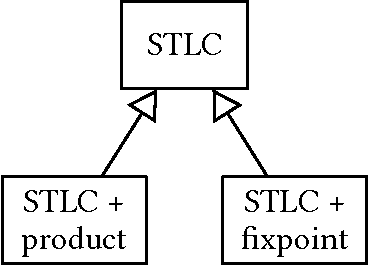
\includegraphics[scale=.48]{graphics/stlc-intro.pdf}
\end{wrapfigure}

%\noindent
%As an example, consider \cref{fig:STLC-example}, the simply typed
%lambda calculus (STLC) mechanized in Coq.
%A programming challenge there is to define distinct extensions of this
%STLC formalization to support distinct features,
%and then selectively compose these extensions to form new STLC variants.
As an example, the diagram to the right depicts an extensible
mechanization of the simply typed λ-calculus (STLC), using family
polymorphism.
An extension of STLC with products and another with fixpoints
can both inherit from the base STLC family:
they reuse mechanized metatheories,
from abstract syntax all the way to the type-safety theorem,
only adding new constructors to inductive types
and adding new cases to recursive functions and induction proofs
\emph{as needed} by an extension.

Integrating family polymorphism into a dependent type theory for
logical reasoning, however, poses significant technical challenges.
As we analyze, pillars of dependent type theories—including
inductive types, definitional equality, and logical consistency—are
all inimical to the kind of extensibility and family polymorphism
found in existing OO language designs.
Thus, our contributions include novel design recipes for dealing with
these challenges and strong meta\-theoretical guarantees on the
underlying logic.
%
Specifically, we make the following contributions.

\endgroup

\begin{itemize}[leftmargin=3.5ex]

\item We present a
%\EDJ{Are you sure? This claim is so bold.}\YZreply{Is there any previous language designs in this space?}\EDJreply{Olivier Boite. 2004. Proof reuse with extended inductive types. In International Conference on Theorem Proving in
%Higher Order Logics. Springer, 50–65.  I think I also mentioned several paper in the related work.}
language design that enables extensible
metatheory mechanization in a higher-order, dependent type theory with
inductive types (\cref{sec:lang-design}).
The language design reconciles the expressiveness enabled by
family polymorphism with the rigor of a proof assistant,
while retaining an idiomatic programming style.

\item We contribute a prototypical implementation of our language
mechanism as a Coq plugin (\cref{sec:coqimpl}). The plugin works by
compiling surface-language definitions into Coq modules parameterized by
explicit extensibility hooks.

\item We capture the essence of the new language mechanism formally by extending
Martin–Löf type theory with facilities to express family polymorphism (\cref{sec:metatheory2}).
We prove foundational meta\-theoretical results including consistency
and canonicity.
%\EDJ{I will suggest use ``foundational'' instead. Sterling at some places say canonicity is the most basic meta-theoretical property.}
%We also formalize the translation implemented by the Coq plugin.

\item We present case studies of using our Coq plugin to mechanize
language metatheories (\cref{sec:casestudies}).
They show how our language design naturally solves the EP and
enables a high degree of reuse and extensibility
for proof engineering.

\end{itemize}

%\paragraph{Structure of the paper} We will quickly introduce Family
%Polymorphism and the challenges to adapt it into dependent type setting
%in \cref{sec:background+challenge}. After that, we will talk about the
%language design of family polymorphism in dependent type setting and the
%implementation of our Coq plugin in \cref{sec:coqimpl}. Then, we
%consider the meta-theory of incorporating family polymorphism into
%predicative MLTT, and deriving consistency and canonicity results in
%\cref{sec:metatheory}. \ref{sec:related-work} discusses related works
%and \ref{sec:conclusion} concludes.




% Concept 
% Contribution

\section{Language Design}
% what feature we want
% what problem/formalization we want to achieve
% Before/After Comparison of examples (with/without Fampoly)
\label{sec:lang-design}
\subsection{Design Space}\YZ{I was thinking if the paper should start by talking about the functional encoding of inheritance (namely exposing a self parameter to allow late binding, and later taking the fixpoint of the extensible module when it needs to be accessed outside the family).  I think most readers will benefit from a recap of this encoding.\\
Coq is total but that doesn’t prevent Coq from having a Fixpoint keyword (plus you proved your language is consistent).
}

When adapting Family Polymorphism into dependent types, we choose to
focus only on the essence of family (and inheritance)
structure in \citet{zm2017}, and thus a lot of unrelated features, like
Interface, will be removed. In this case, it will look like module with
late-binding. Inheritance can be considered as code and proof reuse mechanism for module. We also
need it to have good compatibility with inductive types, because we
don't want to diverge too much from the routine Coq programming experience\YZ{By 'reasoning power of Coq', I suppose you mean the expressive power of Gallina?}\EDJreply{I think the sentence last time was not really making sense because using Church Encoding of inductive doesn't sabotage the expressiveness. I rephrase it now, please check.}
(and its tactic programming). 

Let's start with a basic example---STLC and its extension in
\cref{fig:STLC-example}---to consider what kind of features are required
and how much of them can be supported by family polymorphism.
% add the example code here

\begin{figure}[!htb]
  \begin{minipage}[t]{0.47\linewidth}
\begin{minted}[fontsize=\footnotesize,escapeinside=||]{Coq}
Family STLC.|\YZ{Does minted support adding extra keywords such as 'Family' and 'extends'?}|
Inductive ty : Set :=
  | unit : ty
  | arrow : ty -> ty -> ty.
Inductive term : Set := 
  | var : id -> term 
  | lam : id -> term -> term ...
Fixpoint subst 
  : id -> term -> term := ...
Inductive has_type 
  : context -> term -> type := ...
Proposition subst_lemma :
  has_type (Γ; x ↦ A) t T ->
  has_type Γ u A ->
  has_type Γ (subst x u t) T.
Inductive step : term -> term -> Prop 
  := ...
(* ... and more, end with type safety *)
EndFamily.
\end{minted}
  \end{minipage}
  \begin{minipage}[t]{0.47\linewidth}
\begin{minted}[fontsize=\footnotesize]{Coq}
Family STLC_bool extends STLC.
Extend Inductive ty : Set :=
  | bool : ty.

Extend Inductive term : Set := 
  | tt : term | ff : term 
  | tif : term -> term -> term -> term
Extend Fixpoint subst (* Need to handle new term *)
  : id -> term -> term := ...
Extend Inductive has_type (* .. and new ty too *)
  : context -> term -> type := ...
Extend Proposition subst_lemma :
  ... (* Need to prove extra cases *)


Extend Inductive step : term -> term -> Prop 
  := ... (* Need to expand this binary relation *)
(* ... and more extension *)
EndFamily.
\end{minted}
  \end{minipage}
  \caption{Example STLC and its extension}\label{fig:STLC-example}
\end{figure}



First and foremost, we don't want to throw away some basic good
properties of Coq. \textlabel{Req~(0A)}{langdesign-req0}~\textbf{we
want to retain incremental (modular) type checking}. Notice that, the
modularity here in Coq is a bit different from other languages, because
Coq supports \textit{interactive} theorem proving, so we actually need
\textit{statement-wise} incremental type checking, not only for avoiding
re\-compilation, but also to enable immediate feedback and incremental
type-checking for the Coq developer. We don't want our family to ruin
this conventional routine of interactive development.
\textlabel{Req~(0B)}{langdesign-req0b}~\textbf{we also want to keep the
computational ability of Coq when using families}. Coq, based on constructive
logic, can consider proof as programs. 
We don't want our Family facility to ruin this when incorporated with 
the remaining parts of Coq: 
the developers should be able to project fields of families 
as first-class value just like how they can project fields of Coq's Module.

% We want to reason about fields in a family.
\textlabel{Req (1)}{langdesign-req1}:\textbf{ we want to be able to
reason about fields in a family}, just like in a module, where a field
can reason about its former fields. More generally, we want to allow a
later field to be type-dependent on the former fields. In the example of
\cref{fig:STLC-example}, "subst", "has_type", "subst_lemma" all require
this feature.\YZ{rephrase Req to Challenges}\EDJreply{But it is not really challenge because I didn't show their difficulty. It is more like requirements.}

% we want extensible inductive type
\textlabel{Req (2)}{langdesign-req2}:\textbf{ we need extensible
inductive types}, to extend "term" and "ty" in \cref{fig:STLC-example}.
Extensible inductive types are not supported by \citet{zm2017}, so
we need further consideration about it on both implementation and
metatheory.

\textlabel{Req (3)}{langdesign-req3}: \textbf{we also want extensible
pattern matching and induction reasoning}, to extend "subst" in
\cref{fig:STLC-example}.
There are actually two kinds of ``pattern matching'', one for data and
the other for induction reasoning, i.e., one uses the eliminator to
\mintinline{Coq}{Set} or \mintinline{Coq}{Type}, and the other uses the
eliminator to \mintinline{Coq}{Prop}. Luckily, in this setting,
extensible pattern matching can be easily expressed with family
extension---we just aggregate all case handlers of pattern matching
into one family (as a bunch of functions), and then one family can
encode one pattern matching, and family inheritance can express adding
case handlers. Then we just need to introduce a primitive that will
``wrap'' that family into a recursive function. Induction reasoning can
be handled in an almost identical way. 

% we want to be able to reason pattern matching as well
However, there is still difference between data recursion and induction
reasoning, because the former one is \textit{proof-relevant}. This
difference leads to another issue: \textlabel{Req (4)}{langdesign-req4}:
\textbf{we need to reason about (the computation about) extensible
pattern matching}, just like "subst_lemma" in \cref{fig:STLC-example}.
When proving "subst_lemma", we have to know "subst" is invariant on
"tt", i.e., \mintinline{Coq}{(subst i x tt) = tt}. This kind of
information requires exposing \textit{computational rules} from the
recursors.\YZ{What goes wrong if subst is not invariant or you do not
know whether subst is invariant?}\EDJreply{Then it is unprovable because substitution lemma need to know this. You can just instantiate the whole lemma -- we want  
has_type (Γ; x ↦ A) tt T ->
has_type Γ u A ->
has_type Γ (subst i x tt) T. But this final goal requires to know the
computation of subst.}\YZreply{Seems like what's missing here is to
convince the reader why exposing the definition of subst could be a
problem for family polymorphism.}

% we want tactic programming and certain level of automation
Finally, \textlabel{Req (5)}{langdesign-req5}: \textbf{we desire tactic
programming} to relieve us from the hassle of direct manipulation of proof terms.

\subsection{Language Design}
Inspired by our above requirements and Family Polymorphism, we propose
the following extension to Coq's Vernacular Commands.
% basically write down the specification of surface Coq commandline
%   and then explain  how the language design makes the programmer’s life easier
\begin{align*}
  V := \quad &"Family"~\langle ident\rangle~["extends"~\langle ident\rangle] 
  \quad |\quad "EndFamily" \\
  & |\quad "FRecursor"~\langle ident\rangle~"about"~\langle ident\rangle~"motive"~\langle term\rangle~"using"~\langle ident\rangle \\
  & |\quad "Extend"~"Family"~\langle ident\rangle \\ 
  & |\quad ["Extend"]~"FInductive"~\langle ident\rangle \\ 
  & |\quad ["Final" | "Override"]~"Field"~\langle ident\rangle~":"~\langle term \rangle~":="~\langle term \rangle \\
  & | \quad "Inherit"~\langle ident\rangle \quad | \quad "Inherit Until"~\langle ident\rangle
\end{align*}

We use "Family" and "EndFamily" to scope, and "Field" is used to declare new field members in family.\YZ{This sentence sounds a bit recursive}\EDJreply{What about now?}
We can define nested families.
Family will also be used to encode recursive handlers. Each case
handling of one inductive type will be aggregated into one family, then
"FRecursor" will be used to construct a recursor using these handlers.
For example, \mintinline{Coq}{FRecursor recur about T motive f} "using"
"handlers" will generate a new field "recur" that is doing induction
(using elimination principle of "T") using motive "f", and the handlers
are located in the family "handlers".

We can inherit a top-level family "parent" using \mintinline{Coq}{Family
... extends parent} as a new top-level family. As expected, "Override"
will override a field from the parent. "Inherit" can be used to inherit
nested families, inductive types, and fields. The fields inside a family
are order-sensitive because we have dependent types here. So "Inherit
Until" is used if the user wants to inherit a range of fields. If the
user wants to extend an inductive type or a nested family from the
parent, then "Extend FInductive" or "Extend Family" is used. Thus nested
family can only be inherited or extended together with its outer family
(and thus top level family), thus our support of family polymorphism is
incomplete.

This incomplete support can already be useful for extending functions.
Take \cref{fig:plugin-example2} as example, if we want to extend boolean
inductive type and its negation, we only need to specify the new
constructor for boolean and how negation deals with the new constructor.
As a result, the programmer does not have to duplicate code---otherwise
the user will need to copy and paste the whole original negation
definition and add a new pattern matching case.




% Macro for all use

\newcommand{\denotes}[1]{{\llbracket {#1} \rrbracket}}
\newcommand{\denotesS}[1]{{{\llbracket {#1} \rrbracket}_S}}
\newcommand{\goodCtx}[2]{{ {#1} \ \vdash }}
\newcommand{\goodType}[3]{{ {#1} \vdash {#2} }}
\newcommand{\goodTerm}[3]{{ {#1} \vdash {#2} : {#3} }}
\newcommand{\goodSub}[3]{{ {#1} \vdash {#2} : {#3} }}
\newcommand{\goodSig}[3]{{ {#1} \vdash {#2} \ \  Sig^{#3} }}
\newcommand{\goodWSig}[3]{{ {#1} \vdash {#2} \ \ WSig^{#3} }}
\newcommand{\goodSeal}[4]{{ {#1} \vdash {#2} : {#3} \  |\  {#4} }}
\newcommand{\goodInh}[4]{{ {#1} \vdash {#2} : {#3} \twoheadrightarrow {#4}}}
\newcommand{\nat}{\mathbf{N}}

\newcommand{\cU}{{\mathcal{U}}}
\newcommand{\cB}{{\mathbb{B}}}
\newcommand{\cL}{{\mathcal{L}}}
\newcommand{\cC}{{\mathcal{C}}}
\newcommand{\cCt}{{\mathcal{C}_t}}
\newcommand{\bW}{{\mathbb{W}}}

\section{Prototypical Coq Implementation}
% we need to make this section before Metatheory
% because a lot of our formulation in the metatheory
%   is inspired by the implementation
\label{sec:coqimpl}
We implement our language design as a Coq plugin.
Rather than modifying the Coq kernel, a prototypical implementation as a
plugin allows a clearly defined trusted base and
improved compatibility with different versions of Coq.

The implementation works by translating programs in \Lang syntax into
programs that can be checked and evaluated by Coq.
The translation is compatible with interactive theorem proving (\ref{chg:tooling}), in that
a family is translated piece by piece, allowing each field to be defined
and checked separately.
The translation is modular and efficient, in that
code compiled for fields of a base family
can be shared with derived families without having to be rechecked.

\noindentparagraph{Explicit self parameterization.}

The spirit of the translation is to take ``family polymorphism''
literally: every field is translated into a Coq definition that is
polymorphic to (i.e., universally quantified over) a representation of
its enclosing family.
While this universal quantification has been implicit with the \Lang
syntax, it has to be made explicit in the translated Coq code.

\cref{fig:stlc-compiled,fig:stlcfix-compiled} illustrate the translation of the
\lsti{STLC} and \lsti{STLCFix} families from \cref{fig:stlc-mechanized}.
Fields of a family are translated into parameterized Coq modules
(or parameterized module types).

As an example,
consider field \lsti{env} in family \lsti{STLC}.
It is translated into a top-level module named \lsti{STLC\_env}.
This module has a parameter called \lsti{self} representing the enclosing
family: fields of the current family in the context of \lsti{env} can be
referenced through \lsti{self}.
In particular, \lsti{env} is defined as \lsti{id}\,\lsti{->}\,\lsti{option ty},
where \lsti{ty} is a late-bound reference to the \lsti{ty} field of the
enclosing family.
Hence, this reference to \lsti{ty} is translated to \lsti{self.ty},
which is manifestly polymorphic to the enclosing family.
This translation of the \lsti{env} field can be shared
with a derived family even if it extends \lsti{ty} (e.g., \lsti{STLCProd})---%
no recompilation is needed because \lsti{self.ty} is not tied to any
concrete definition of \lsti{ty}.

The type of \lsti{STLC\_env}'s \lsti{self} parameter is \lsti{STLC\_env\_Ctx},
a module type constructed from \lsti{STLC\_ty}, 
the translation of the field before \lsti{env},
and its context \lsti{STLC\_ty\_Ctx}.
In turn, \lsti{STLC\_ty\_Ctx} (not shown in \cref{fig:stlc-compiled}) is
constructed from \lsti{STLC\_subst},
the translation of the field before \lsti{ty},
and its context \lsti{STLC\_subst\_Ctx}.
Thus, the \lsti{self} parameter can be used to reference those and only
those fields in the current field's typing context, which echoes the
discussion in \cref{sec:sound}.

\begin{figure}
\vspace{-5pt}
\begin{minipage}{\textwidth}
\begin{multicols}{2}

\lstset{
  basicstyle=\fontsize{8}{8.2}\ttfamily,
% numbers=left,
}

\colorlet{codecomment-color}{dkgreen}

\newcommand{\innersep}{\vspace{6pt}}
\newcommand{\outersep}{\vspace{5pt}}
\newcommand{\outdent}{\!\!\!}

\begin{lstlisting}
[@\outdent@][@\codecomment{Code emitted upon definition of \texttt{tm} in family \texttt{STLC}}@][@\tanc{c-STLC-tm-start}@]
[@\outdent@]Module Type STLC\_tm\_Ctx.
[@\outdent@]End STLC\_tm\_Ctx.[@\innersep@]
[@\outdent@]Module Type STLC\_tm (self : STLC\_tm\_Ctx).
Axiom tm : Set.
Axiom tm_unit : tm.[@\hfill@]Axiom tm_var : id -> tm.
Axiom tm_abs : id -> tm -> tm.
Axiom tm_app : tm -> tm -> tm.
Axiom tm_prect_STLC : [@\dadada@].
Axiom [@\textls[-30]{tm\_unit\_eq\_STLC}@][@\;:\;@][@\dadada@]. Axiom [@\textls[-30]{tm\_abs\_eq\_STLC}@][@\;:\;@][@\dadada@].
Axiom [@\textls[-30]{tm\_abs\_eq\_STLC}@][@\;:\;@][@\dadada@].  Axiom [@\textls[-30]{tm\_app\_eq\_STLC}@][@\;:\;@][@\dadada@].
[@\outdent@]End STLC\_tm.[@\tanc{c-STLC-tm-end}@][@\outersep@]
[@\outdent@][@\codecomment{Code emitted upon definition of \texttt{subst} in family \texttt{STLC}}@][@\tanc{c-STLC-subst-start}@]
[@\outdent@]Module Type STLC\_subst\_Cases\_Ctx.
Include STLC\_tm\_Ctx.  Include STLC\_tm.
[@\outdent@]End STLC\_subst\_Cases\_Ctx.[@\innersep@]
[@\outdent@]Module [@\textls[-30]{STLC}@]\_[@\textls[-30]{subst}@]\_[@\textls[-30]{Cases}@] (self[@\,@]:[@\,@][@\textls[-30]{STLC}@]\_[@\textls[-30]{subst}@]\_[@\textls[-30]{Cases}@]\_[@\textls[-30]{Ctx}@]).
Def subst\_tm_unit :=
  \lambda (x : id) (t : self.tm), self.tm_unit.
Def subst\_tm_var := [@\dadada@].
Def subst\_tm_abs := [@\dadada@].  Def subst\_tm_app := [@\dadada@].
[@\outdent@]End STLC\_subst\_Cases.[@\innersep@]
[@\outdent@]Module Type STLC\_subst\_Ctx.
Include STLC\_subst\_Cases\_Ctx.
Include STLC\_subst\_Cases.
[@\outdent@]End STLC\_subst\_Ctx.[@\innersep@]
[@\outdent@]Module Type STLC\_subst (self : STLC\_subst\_Ctx).
Axiom subst : self.tm[@\,@]->[@\,@]id[@\,@]->[@\,@]self.tm[@\,@]->[@\,@]self.tm.
Axiom subst_tm_unit_eq :
  \forall x t, self.subst (self.tm_unit) x t =
  self.subst\_tm_unit x t.
Axiom subst_tm_var_eq : [@\dadada@].
Axiom subst_tm_abs_eq : [@\dadada@].
Axiom subst_tm_app_eq : [@\dadada@].
[@\outdent@]End STLC\_subst.[@\tanc{c-STLC-subst-end}@][@\columnbreak@]
[@\outdent@][@\codecomment{Code emitted upon definition of \texttt{ty} in family \texttt{STLC}}@] [@\tanc{c-STLC-ty-start}@]
[@\dadada@][@\tanc{c-STLC-ty-end}@][@\outersep@]
[@\outdent@][@\codecomment{Code emitted upon definition of \texttt{env} in family \texttt{STLC}}@][@\tanc{c-STLC-env-start}@]
[@\outdent@]Module Type STLC\_env\_Ctx.
Include STLC\_ty\_Ctx.  Include STLC\_ty.
[@\outdent@]End STLC\_env\_Ctx.[@\innersep@]
[@\outdent@]Module STLC\_env (self : STLC\_env\_Ctx).
Def env : Type := id -> option self.ty.
[@\outdent@]End STLC\_env.[@\tanc{c-STLC-env-end}@][@\outersep@]
[@\outdent@][@\codecomment{Code emitted for other fields defined in family \texttt{STLC}}@][@\tanc{c-STLC-rest-start}@]
[@\dadada@][@\tanc{c-STLC-rest-end}@][@\outersep@]
[@\outdent@][@\codecomment{Code emitted upon conclusion of family \texttt{STLC}}@][@\tanc{c-STLC-start}@]
[@\outdent@]Module STLC.[@\innersep@]
Inductive tm\_ : Set :=[@\tanc{c-STLC-d-tm-start}@]
| tm_unit\_[@\,@]:[@\,@]tm\_ | tm_var\_[@\,@]:[@\,@]id -> tm\_
| tm_abs\_[@\,@]:[@\,@]id->tm\_->tm\_ | tm_app\_[@\,@]:[@\,@]tm\_->tm\_->tm\_.
[@\codecomment{Instantiate \texttt{tm} \& its constructors}@]
Def tm := tm\_.
Def tm_unit := tm_unit\_. Def tm_var := tm_var\_.
Def tm_abs  := tm_abs\_.  Def tm_app := tm_app\_.
[@\codecomment{Instantiate \texttt{tm} partial recursor \& its equalities}@]
Def tm_prect_STLC := \lambda P, tm\__rect (\lambda[@\,@]t, option (P t)).
Fact[@\;@][@\textls[-20]{tm\_unit\_eq\_STLC}@][@\,@]:[@\,@][@\dadada@].[@\,@][@\textls[-40]{{\color{dkblue}reflexivity}.}@][@\,@]Qed.[@\hfill@]Fact [@\dadada@][@\tanc{c-STLC-d-tm-end}@][@\innersep@]
Include STLC\_subst\_Cases.[@\tanc{c-STLC-d-subst-start}@]
[@\codecomment{Instantiate \texttt{subst} \& its equalities}@]
Def subst[@\,@] := tm\__rect _ subst\_tm_unit subst\_tm_var
                        subst\_tm_abs  subst\_tm_app.
Fact[@\;@][@\textls[-40]{subst\_tm\_unit\_eq}@][@\,@]:[@\,@][@\dadada@].[@\,@][@\textls[-40]{{\color{dkblue}reflexivity}.}@][@\,@]Qed.[@\hfill@]Fact [@\dadada@][@\tanc{c-STLC-d-subst-end}@][@\tanc{c-STLC-firstcol-end}@][@\innersep@]
[@\codecomment{Instantiate \texttt{ty}, its constructors, partial recusor \& eq.}@] [@\dadada@][@\tanc{c-STLC-d-ty}@][@\tanc{c-STLC-sndcol-start}@][@\innersep@]
Include STLC\_env.[@\hfill\codecomment{Include \texttt{env}}@][@\tanc{c-STLC-d-env}@][@\innersep@]
[@\codecomment{Include/Instantiate other fields of family \texttt{STLC}}@] [@\dadada@][@\tanc{c-STLC-d-rest}@][@\innersep@]
[@\outdent@]End STLC.[@\tanc{c-STLC-end}@]
\end{lstlisting}

\makeline[-1pt]{c-STLC-tm-start}{c-STLC-tm-end}[codecomment-color!50][1.8pt]
\makeline[-1pt]{c-STLC-subst-start}{c-STLC-subst-end}[codecomment-color!50][1.8pt]
\makeline[.5\textwidth+8pt]{c-STLC-ty-start}{c-STLC-ty-end}[codecomment-color!50][1.8pt]
\makeline[.5\textwidth+8pt]{c-STLC-env-start}{c-STLC-env-end}[codecomment-color!50][1.8pt]
\makeline[.5\textwidth+8pt]{c-STLC-rest-start}{c-STLC-rest-end}[codecomment-color!50][1.8pt]
\makeline[.5\textwidth+8pt]{c-STLC-start}{c-STLC-end}[codecomment-color!50][1.8pt]
\makeline[.5\textwidth+12pt]{c-STLC-d-tm-start}{c-STLC-d-tm-end}[codecomment-color!35][1.0pt]
\makeline[.5\textwidth+12pt]{c-STLC-d-subst-start}{c-STLC-d-subst-end}[codecomment-color!35][1.0pt]
\makeline[.5\textwidth+12pt]{c-STLC-d-ty}{c-STLC-d-ty}[codecomment-color!35][1.0pt]
\makeline[.5\textwidth+12pt]{c-STLC-d-env}{c-STLC-d-env}[codecomment-color!35][1.0pt]
\makeline[.5\textwidth+12pt]{c-STLC-d-rest}{c-STLC-d-rest}[codecomment-color!35][1.0pt]

\end{multicols}
\end{minipage}

\vspace{-12pt}

\caption{Compilation of family \lsti!STLC! (\cref{fig:stlc-mechanized}).}
\label{fig:stlc-compiled}
\end{figure}
\begin{figure}
\vspace{-5pt}
\begin{minipage}{\textwidth}
\begin{multicols}{2}

\lstset{
  basicstyle=\fontsize{8}{8.2}\ttfamily,
% numbers=left,
}

\colorlet{codecomment-color}{dkgreen}

\newcommand{\innersep}{\vspace{6pt}}
\newcommand{\outersep}{\vspace{5pt}}
\newcommand{\outdent}{\!\!\!}

\colorlet{codecomment-color}{orange}

\begin{lstlisting}
[@\outdent@][@\codecomment{Code emitted upon definition of \texttt{tm} in \texttt{STLCFix}}@][@\tanc{c-STLCFix-tm-start}@]
[@\outdent@]Module Type STLCFix\_tm\_Ctx.
[@\outdent@]End STLCFix\_tm\_Ctx.[@\innersep@]
[@\outdent@]Module Type STLCFix\_tm (self : STLCFix\_tm\_Ctx).
Include STLC\_tm(self).
Axiom tm_fix : id -> tm -> tm.
Axiom tm_fix_eq_STLC : \forall[@\,@][@\dadada@],[@\,@]tm_prect_STLC [@\dadada@][@\;@]=[@\;@]None.
Axiom tm_prect_STLCFix : [@\dadada@].
Axiom tm_fix_eq_STLCFix : [@\dadada@].
[@\outdent@]End STLCFix\_tm.[@\tanc{c-STLCFix-tm-end}@][@\outersep@]
[@\outdent@][@\codecomment{Code emitted upon definition of \texttt{subst} in \texttt{STLCFix}}@][@\tanc{c-STLCFix-subst-start}@]
[@\outdent@]Module Type STLCFix\_subst\_Cases\_Ctx.
Include STLCFix\_tm\_Ctx. Include STLCFix\_tm.
[@\outdent@]End STLCFix\_subst\_Cases\_Ctx.[@\innersep@]
[@\outdent@]Module STLCFix\_subst\_Cases
[@\outdent@](self : STLCFix\_subst\_Cases\_Ctx).
Include STLC\_subst\_Cases(self).[@\hfill\codecomment{reuse}@]
Def subst\_tm_fix := [@\dadada@].[@\hfill\codecomment{translation of new case}@]
[@\outdent@]End STLCFix\_subst\_Cases.[@\innersep@]
[@\outdent@]Module Type STLCFix\_subst\_Ctx.
Include STLCFix\_subst\_Cases\_Ctx.
Include STLCFix\_subst\_Cases.
[@\outdent@]End STLCFix\_subst\_Ctx.[@\innersep@]
[@\outdent@]Module Type STLCFix\_subst (self[@\,@]:[@\,@][@\textls[-30]{STLCFix}@]\_[@\textls[-30]{subst}@]\_[@\textls[-30]{Ctx}@]).
Include STLC\_subst(self).
Axiom subst_tm_fix_eq : [@\dadada@].
[@\outdent@]End STLCFix\_subst.[@\tanc{c-STLCFix-subst-end}@][@\outersep@]
[@\outdent@][@\codecomment{Code emitted for other fields defined in \texttt{STLCFix}}@] [@\dadada@][@\tanc{c-STLCFix-rest}@][@\outersep@]
[@\outdent\codecomment{Code emitted upon conclusion of \texttt{STLCFix}}@][@\tanc{c-STLCFix-start}@]
[@\outdent@]Module STLCFix.[@\innersep@]
[@\codecomment{Instantiate \texttt{tm} \& its constructors}@][@\tanc{c-STLCFix-d-tm-start}@]
Inductive tm : Set :=
| tm_unit | tm_var (v : id)
| tm_abs (v : id) (b : tm) | tm_app (a b : tm)
| tm_fix (v : id) (b : tm).
[@\codecomment{Inst. \texttt{tm} partial recursors \& their comp.\ behaviors}@] [@\dadada@][@\tanc{c-STLCFix-d-tm-end}@][@\innersep@]
Include STLCFix\_subst\_Cases. [@\tanc{c-STLCFix-d-subst-start}@]
[@\codecomment{Instantiate \texttt{subst} \& its computational behaviors}@]
Def subst := tm_rect _ subst\_tm_unit
subst\_tm_var subst\_tm_abs subst\_tm_app[@\hfill\codecomment{reuse}@]
subst\_tm_fix.
Fact [@\textls[-0]{subst\_tm\_unit\_eq}@] : [@\dadada@]. reflexivity. Qed.
Fact [@\dadada@][@\tanc{c-STLCFix-d-subst-end}@][@\innersep@]
[@\codecomment{\textls[-10]{Include\;\texttt{ty}, its constructors, partial recursor, etc.}}@] [@\dadada@][@\tanc{c-STLCFix-d-ty}@][@\innersep@]
Include STLC\_env.[@\hfill\codecomment{reuse}@][@\tanc{c-STLCFix-d-env}@][@\innersep@]
[@\codecomment{Include/Instantiate other fields of \texttt{STLCFix}}@] [@\dadada@][@\tanc{c-STLCFix-d-rest}@][@\innersep@]
Include STLC\_typesafe.[@\hfill\codecomment{reuse}@][@\tanc{c-STLCFix-d-typesafe}@][@\innersep@]
[@\outdent@]End STLCFix.[@\tanc{c-STLCFix-end}@]
\end{lstlisting}

\makeline[-1pt]{c-STLCFix-tm-start}{c-STLCFix-tm-end}[codecomment-color!50][1.8pt]
\makeline[-1pt]{c-STLCFix-subst-start}{c-STLCFix-subst-end}[codecomment-color!50][1.8pt]
\makeline[.5\textwidth+8pt]{c-STLCFix-rest}{c-STLCFix-rest}[codecomment-color!50][1.8pt]
\makeline[.5\textwidth+8pt]{c-STLCFix-start}{c-STLCFix-end}[codecomment-color!50][1.8pt]
\makeline[.5\textwidth+12pt]{c-STLCFix-d-tm-start}{c-STLCFix-d-tm-end}[codecomment-color!35][1.0pt]
\makeline[.5\textwidth+12pt]{c-STLCFix-d-subst-start}{c-STLCFix-d-subst-end}[codecomment-color!35][1.0pt]
\makeline[.5\textwidth+12pt]{c-STLCFix-d-ty}{c-STLCFix-d-ty}[codecomment-color!35][1.0pt]
\makeline[.5\textwidth+12pt]{c-STLCFix-d-env}{c-STLCFix-d-env}[codecomment-color!35][1.0pt]
\makeline[.5\textwidth+12pt]{c-STLCFix-d-rest}{c-STLCFix-d-rest}[codecomment-color!35][1.0pt]
\makeline[.5\textwidth+12pt]{c-STLCFix-d-typesafe}{c-STLCFix-d-typesafe}[codecomment-color!35][1.0pt]

\vspace{-3pt}

\definecolor{codecomment-color}{HTML}{000080}

\begin{lstlisting}
[@\outdent@][@\codecomment{Code emitted upon command \texttt{\textls[-35]{Check STLCFix.typesafe}}}@][@\tanc{c-Check-STLCFix-typesafe-start}@]
[@\outdent@]Check STLCFix.typesafe.[@\tanc{c-Check-STLCFix-typesafe-end}@]
\end{lstlisting}

\makeline[.5\textwidth+8pt]{c-Check-STLCFix-typesafe-start}{c-Check-STLCFix-typesafe-end}[codecomment-color!50][1.8pt]

\end{multicols}
\end{minipage}

\vspace{-12pt}

\caption{Compilation of family \lsti!STLCFix! and the final \lsti!Check! command (\cref{fig:stlc-mechanized}).}
\label{fig:stlcfix-compiled}
\end{figure}

\noindentparagraph{Translating extensible inductive types.}

An \lsti{FInductive} definition is translated to a parameterized module type.
Consider the inductive type \lsti{tm}.
In \lsti{STLC}, it is translated to a top-level module type
\lsti{STLC\_tm} that declares a \lsti{tm} type,
its constructors (e.g., \lsti{tm_abs}),
its partial recursor (\lsti{tm_prect_STLC}),
and the propositional equalities on the partial recursor
(e.g., \lsti{tm_abs_eq_STLC}; \cref{sec:prec}).

Importantly,
\lsti{STLC\_tm} merely declares the existence of these names and their types;
it does not specify their definitions or proofs.
Knowing the existence of these names and their types
suffices to type-check and translate the rest of the family.
Leaving the definitions and proofs open enables \lsti{STLC} and \lsti{STLCFix}
to instantiate \lsti{tm} differently upon \lsti{End}~\lsti{STLC} and \lsti{End}~\lsti{STLCFix}.

The command \lsti{FInductive tm : Set += tm_fix : }\dadada~in family
\lsti{STLCFix} is again translated to a module type \lsti{STLCFix\_tm} (\cref{fig:stlcfix-compiled}).
It includes all the names declared by \lsti{STLC\_tm}
via command \lsti!Include STLC\_tm(self)!,
and additionally declares
the new constructor \lsti{tm_fix} and related equalities.


\noindentparagraph{Translating recursion and induction.}

An \lsti{FRecursion} definition is translated in two parts:
first a module containing the definitions of all the case handlers,
and then a module type declaring the existence of the recursive function as well as
its propositional equalities.

Consider the translation of \lsti{subst} in family \lsti{STLC}.
First, a module named \lsti{STLC\_subst\_Cases} is generated interactively:
every time the programmer completes a \lsti{Case}, a case handler (e.g., \lsti{Def subst\_tm_unit})
is generated and added to the module.

Upon \lsti{End}~\lsti{subst}, a module type named \lsti{STLC\_subst} is generated.
%
As discussed in \cref{sec:latebind}, \lsti{subst} can be further bound,
so its definition is not exposed to the fields that come after it.
Accordingly, the translation \lsti{STLC\_subst} merely declares the type of \lsti{subst}
and the existence of its propositional equalities, leaving \lsti{subst} undefined
and the equalities unproven.
%
The propositional equalities are stated in terms of the case handlers,
whose definitions \emph{are} available through the \lsti{self} parameter.
So Coq can simplify, for example, \lsti{subst_tm_unit_eq}'s type to
\lsti!\forall x t, self.subst self.tm_unit x t = self.tm_unit!.
The equalities will be included and available for use in the
translations of the subsequent fields through their \lsti{self}
parameters.

Importantly, code generated for the case handlers is shared with derived families.
In \cref{fig:stlcfix-compiled}, module \lsti{STLCFix\_subst\_Cases}
reuses---without rechecking---all the case handlers in
\lsti{STLC\_subst\_Cases} via command \lsti{Include STLC\_subst\_Cases(self)}.

The translation of \lsti{FInduction} is similar, except that there is no need to
register propositional equalities, as \lsti{FInduction} proofs are considered opaque.


\noindentparagraph{Translation of further-bindables vs.\ non-further-bindables.}

In family \lsti{STLC},
field \lsti{env} and the case handlers for \lsti{subst}
are not further-bindable by derived families.
In contrast, \lsti{tm}, \lsti{subst}, and the related equalities
can be further bound.
The distinction is reflected in the translations.
The further-bindable fields are translated to module types that export only types of the fields.
The non-further-bindable fields are translated to modules that export definitional equalities
on the fields.
Opaque fields can be further bound, too (\cref{sec:override});
they are translated to modules that export opaque fields.

%\footnotetext{%
%Axioms in Coq module types are more like parameters than real axioms.
%They become part of the signature described by the module type.
%}


\noindentparagraph{Eliminating \lsti{self} by aggregation.}

Upon the conclusion of a family definition,
a representation of the family is created.
For example, module \lsti{STLC} in \cref{fig:stlc-compiled} is generated
upon \lsti{End}~\lsti{STLC}.
%
This module can be viewed as the ``fixed point'' of the
\lsti{self}-parameterized translations.
The ``fixed point'' is taken step by step, by adding the translation of
each field to this module in the same order as they appear in the family
definition.

For the non-further-bindables, the translated modules are directly included
(e.g., \lsti{Include STLC\_env} and \lsti{Include STLC\_subst\_Cases} in \cref{fig:stlc-compiled}).
%
The instantiation of \lsti{self}s for these modules is implicit, thanks to a Coq nicety:
when including a higher-order module, Coq automatically instantiates its
parameter with the current interactive module environment.
For instance, command \lsti{Include STLC\_subst\_Cases} is successfully executed,
because Coq automatically instantiates the \lsti{self} parameter using the current
module environment, which by construction contains all the fields required by \lsti{STLC\_subst\_Cases\_Ctx}.

For the further-bindables, \lsti{Axiom}s declared in the module types must be instantiated.
%
\begin{itemize}
  [align=left,itemsep=2pt,labelsep=*,leftmargin=*]

\item
In \cref{fig:stlc-compiled},
an inductive type \lsti{tm} is generated, instantiating the axiomatized
\lsti{tm} type and its constructors.
%
The partial recursor \lsti{tm_prect_STLC} is defined
%to \lsti{\lambda}\,\lsti{P, tm_rect (\lambda}\,\lsti{t, option (P t))},
with the help of \lsti{tm_rect}, the recursor Coq generates for \lsti{tm}.
Proving the equalities on \lsti{tm_prect_STLC} is then trivial, by \lsti{reflexivity}.

\item
Similarly, \lsti{subst} is instantiated by applying the recursor \lsti{tm_rect}
to the (already included) case handlers. %(\lsti{subst\_tm_unit}, etc.).
Propositional equalities on \lsti{subst} are then trivial, by \lsti{reflexivity}.

\end{itemize}

Module \lsti{STLCFix} in \cref{fig:stlcfix-compiled} is emitted upon
\lsti{End}~\lsti{STLCFix}, in the same way as described above for \lsti{STLC}.
The translation makes sharing evident.
In particular, case handlers compiled for \lsti{STLC}
are reused to instantiate \lsti{subst}, \lsti{substlem}, and alike.
\lsti{STLC\_env} and \lsti{STLC\_typesafe}
are also reused in the construction of module \lsti{STLCFix}.
%
One may argue that since the first four constructors of \lsti{tm} are
repeated in \lsti{STLCFix}, the translation does not satisfy the
modular compilation requirement.
We could address this concern by using wrapper types,
but we consider restating constructors a small price to pay in return
for the clarity and concision of implementation.
We emphasize that compiled case handlers, such as \lsti!subst\_tm_abs!,
are entirely reusable without rechecking, even with restated constructors.
%
Finally, the reference \lsti{STLCFix.typesafe} (where \lsti{STLCFix} is a family)
can simply be translated to \lsti{STLCFix.typesafe} (where \lsti{STLCFix} is a Coq module),
as the last line of \cref{fig:stlcfix-compiled} shows.

\ifShowOldWriting

\newpage

In this section, we describe how we can implement the proposed Vernacular commands.

After considering the pros and cons, we decide to implement a Coq Plugin where we can add new Vernacular commands and translate each new command into a bunch of Coq commands (the orignal surface Vernacular command) on the fly, instead of modifying the code-base of Coq. 

Despite possible difficulties for future maintenance, this approach has
various advantages: 1. it is the easiest and the most accessible way to
prototype as it relieves us the necessity of familarity of Coq base,
especially for the implementation of the module and functor; 2. we have
a clear definition of trusted-base---the whole Coq; 3. it is easy to
debug---we just need to check the translated commands; 4. it can be
well-incorporated with the existent tools like VSCoq; 5. it is more
accessible for the interested audience who can then easily adapt our
plugin and give a try---otherwise they have to download and re-build the
whole customized Coq; 6. it is more stable because the surface syntax of
Coq should be stable across different versions; 7. still, this plugin
can capture the key ingredients of implementing family polymorphism
inside Coq and act as a reference for guiding an appropriate
implementation of Family Polymorphism inside all sorts of proof
assistants.\YZ{Does the Coq implementation perform type checking to
prevent illegal uses fam poly?}\EDJreply{Yes. Because I define feature of fampoly as a direct translation into Coq feature.  The fampoly is like a shorthand into multiple Coq commands. \\
Do you find translation from my current metatheory into MLTT (without linkage) helpful? \\
Actually I am also not sure what this question is aiming towards. \\
Are you complaining there is no formal specification of my fampoly feature in paper and thus there is no proof my Coq surface syntax is related to metatheory? If so, I thought our Coq plugin is only advertising how powerful Fampoly is to solve expression problem in mechanized proving. I can decouple the relationship between our plugin and our metatheory if you find the gap is really there... And I can only claim metatheory is about a partial result on incorporating fampoly with dependent type, Coq plugin is using two example to illustrate how mechanized proving can get benefit and our Coq plugin is only inspired by our metatheory (and not claim any relationship). Doing so would require rearrange the metatheory section before this section. \\
But I don't think the gap is there at all because if you want all possible gaps to disappear, then the action of using debruijn is wrong because we need to prove the one using debruijn and the surface syntax that is not using debruijn are ``equivalent''. What's more, module is not sigma type because Module is not a term in Coq and thus there is no formalism of Module at all. Let alone I don't see the plausibility of mechanizing dependent type without debruijn. \\ 
Please comment back so that I know what corresponding modification is needed on the paper. 
}\YZreply{My original question was more directed towards the fact
that currently type checking is deferred to the Coq base. Generally,
when one uses a statically typed language as a compilation target, they
also want to have type checking at the source level, (1) because there
could be type errors at the source level that could not otherwise be
caught at the target level and (2) because it allows better error messages.
So it needs to be addressed why deferring type checking to Coq is OK.}\EDJreply{Good point. I think (1) is largely mediated by the fact the semantic of family is very close to that of the module. And the supporting feature is simple enough that there won't appear some problems like type error at source-level but not target level(2) is happening for sure but some basic error message is almost "transparent" i.e. the error-messages from Coq can be directly interpreted for the user. But my justification is solely empirical and as you know the empirical study for this paper is not really strong enough to support anything.}


\textbf{Family compiled into module.} The main idea of our plugin is to support family by compiling
family components into Coq modules, family ``types'' into module types, and the context of a given term
into parameters of the module. 

Since by default every field is inheritable, for each defining field (informally) $ .. \cL\sigma \vdash t : T $, we need to compile $t$ using
``universal-quantifier-wrapped term'' : $.. \vdash \lambda t : \forall
\cL \sigma. T$, so that field $t$ can be inherited to all the future family with strengthen context $\sigma^+$ with the help of weakening from $\sigma^+$ to $\sigma$.  However, instead of using Coq's universal quantifier, we choose module and module parameters to achieve this wrapping---each
family type in the context will be one module parameter
with the compiled module type, and thus each field of the family will
compile into a functor parametrized by its context. Doing so we can also
get rapid feedback from type checking when the users are defining each
field interactively with Coq. Note that, when compiling the context during the  compilation of a default (non-overridable)  field, all the default (non-overridable) former fields will expose their definition in the context while overridable fields will only expose their types.
% Insert one pseudo-code example for explanation of the mechanism
\begin{figure}[!htb]
  \begin{minipage}[t]{0.30\linewidth}
\begin{lstlisting}[language=Coq, escapeinside={@}{@}]
Family A.
Field a : nat := 1.
Field b : a = 1 := eq_refl.
Overridable Field a' : nat 
                     := 1. 
Overridable pins {a'}
  Field b' : a' = 1 
          := eq_refl.
EndFamily.
\end{lstlisting}
  \end{minipage}%\YZ{Can the self's be omitted?}\EDJreply{Yes. But in our current plugin implementation it is not omitted. I think altering example is fine. If you think some small distance between example and the current implementation is fine, please comment back and I will remove all the self_}\YZreply{If omitting the self's poses no technical challenges, then I'd say it's fine to also omit them in this figure.}\EDJreply{Omitting self_ is easy and not much engineering effort is required. But omitting self_ will lead to `A.a' instead of `a' actually. So if we really want `a' as you last time mentioned, then a resolution is required and more engineering effort is required. But I don't see any technical difficulties. I have removed all the self, please check.}
  \begin{minipage}[t]{0.35\linewidth}
\begin{minted}[fontsize=\footnotesize]{Coq}
Module a_4 (self_A: EmptySig).
Definition a : nat := 1. End a_4.
Module Type a_6.
Include a_4. End a_5.
Module b_7 (self_A: a_6).
Definition b 
  : self_A.a = 1
  := eq_refl. End b_7.
Module Type b_9.
Include a_6. Include b_7. End b_9.
Module a'_10 (self_A: b_9).
Definition a' : nat := 1. End a_4.
\end{minted}
  \end{minipage}
  \begin{minipage}[t]{0.3\linewidth}
\begin{minted}[fontsize=\footnotesize]{Coq}
Module Type a'_12.
Include b_9. Include a'_10. End a'_12.
Module b'_16 (self_A: a'_12).
Definition b' : self_A.a' = 1 := eq_refl. End b'_16.
Module Type b'_19.
Include b_9. Parameter a': nat.
Parameter b': a' = 1. End b'_19.
Module test_20 (self_A: b'_19).
Definition test : nat := 1. End test_20.

Module A. (* Final Aggregation *)
Include a_4. Include b_7. Include a'_10.
Include b'_16. Include test_20. End A.
\end{minted}
  \end{minipage}
  \caption{Example Code and Plugin Translation}\label{fig:plugin-example1}
\end{figure}


% Concrete details of compilation of a family term data structure
Taking \cref{fig:plugin-example1} as an example: immediately after the user inputs the line "Field a : nat := ..", our plugin will
translate this statement into the "Module a_4", "Module Type a_6"
two components.
{The "EmptySig" is just an empty module type.} Then,
these modules and module types will be generated and type-checked by Coq
immediately. The compiled "Module a_6" is then part of the context of
"Field b" (as the module type of "self_A") for "b" to refer to, so that "b" knows "a"'s concrete definition. The
internal representation of family "A" is the list of these
compiled modules and module types. We can achieve incremental
checking as in \ref{chg:software-engineering}. This makes all kinds of inheritance plausible---for example, if we
want to override "Field a", we simply replace that compiled module with
the new module inside the list. 
% This compiled module type serves as an abstraction that enables overriding. 



After closing the top family, the user can access family "A" like it is a module. This is achieved by a complete compilation from a family to a module,
via aggregating the list of the modules in the internal representation:
the plugin will repeatedly using Coq's "Include" command as the "Module
A" as \cref{fig:plugin-example1} illustrates.
References to family "A" outside "A" will be compiled to references to
this Coq module "A".

Note that, in our example, we include two
functors without arguments---this is due to a peculiarity of Coq's
"Include": uninstantiated parameters will be automatically
instantiated by the appropriate fields in the surrounding defining
module.
For example, "b_7" requires a module of type "a_6". Inside module "A",
when "Include a_4" is done, we will have a field \mintinline{Coq}{a : nat := 1}
inside the current surrounding "A". Then when we
\mintinline{Coq}{Include b_7} without specifying the module parameter,
Coq will try to find fields in the surrounding module (i.e., module
"A") to instantiate \mintinline{Coq}{self_A: a_6}. This is satisfied by
the \mintinline{Coq}{a : nat} that is included earlier.
The resulting compiled module is just like mundane Coq's module and 
thus maintains all the computational mechanism from Coq, fulfilling
requirements in \ref{chg:software-engineering}.\YZ{
  Do I understand correctly that an alternative to individually
  compiling family members to modules is to compile a family as a whole,
  but this alternative would not satisfy the "incremental type checking"
  or "instant feedback" requirement?
}\YZreply{
  Looks like individually compiling family members addresses not only
  this requirement, but also the "self vs. consistency" challenge.
}\EDJreply{Yes. Indivially compiling family member can achieve both requirements}

\textbf{Implementing "Overridable" and Overriding Chain.}
We implement "Overridable" by simply annotating the corresponding field type with a mark and its dependency. Then when compute the context during the compilation of the term for that field, we make sure only all the dependee and the non-overridable field will expose its definition in the context. 

Most parts of the implementation is quite similar to the default fields, except that when inheriting an overridable field, we need to make sure all its dependee is inherited earlier.  For example, in \cref{fig:plugin-example1}, the module "b'_16" will compile "b'" in the context of "a'_12" where the concrete definition of "a'" is exposed since "b'" depends on "a'"; while the module "test_20" is compiled in the context "b'_19" only knowing the type of "a'" and "b'".

When aggregating the overridable fields into a module, since everything has concrete definition now, there won't be any problem---we just use the same way that aggregates the default fields.



% explaining inheritance
\textbf{Implementing Inheritance.}
To simplify the implementation, we can consider all families as
inheritance and the standalone families are extending the empty family.
Thus, we need to deal with only inheritance during interactive theorem proving.


Simiarly, we
use a list to encode the three kinds of inheritance data in the
implementation. The inheritance data will include the
information of (1) the ``type'' of the parent family, (2) a list of
operation indicating how each field of the parent will be dealt with
(either inherited or overriden), (3) the operations indicating newly
extended fields, and (4) the ``type'' of the children family.
The surface syntax for the three kinds of inheritance
are demonstrated in the exemplar \cref{fig:plugin-example3}. The
implementation of overriding, inheritance, and extension is achieved by
simply manipulating the internal representation of a family
correspondingly---we can swap the module in the list for overriding,
retain the module in the list for inheritance, and add new module into
the list for extension. The compilation from a family (internal
representation) to a module still acts the same.

Though inheritance is solely a first-order data rather
than a ``mapping'', it is still possible to \text{mixin} two inheritance
data---by carefully ``mix'' the internal list, we can compose the
inheritance. However, a good definition of mixin is still under
investigation. We will show one practical example of \textit{mixin}
later.\YZ{How about making mixin composition one of your Req's? Also
does any example in the paper illustrate how to do this?}\EDJreply{mixin
is not really formalized. There is no example illustrate it. The only
example is the STLC example at the very end and I just kind of
``mention'' it. I think here I just want to emphasize, inheritance as
first order data is still possible to support composition.}

Our implementation also makes sure the first attempt of defining "c"
failed successfully in \cref{fig:plugin-example3}---proving "c"
would require a concrete definition of "a", and our plugin rejects
\mintinline{Coq}{c : a = 1 := eq_refl} in a context where we
only know \mintinline{Coq}{a : nat}.



% \textbf{Implementing "Final" and "Sealed Family".}
% We implement "Final" by
% exposing the whole definition directly into the compiled module type.
% Doing so will prohibit overriding. Say, "bop", declared "Final" in
% \cref{fig:plugin-example3}, is not overridable.
% We require the users to manual decorate field as `Final' so that the
% plugin will proceed with this special treatment.
% %\YZ{This para is confusing: which kind of equality is used, propositional or judgmental? Where does 'Final' show up in the example?}\EDJreply{I rephrase it and remove the part on talking about meta-theory. Now everything is about judgemental so I don't have to emphasize judgemental. I wanted to make the example small but I guess I can add one `Final' statement into our example. Don't resolve it until I add it into Figure 2.}

% % \textbf{Special Fields: Overridable/Sealed Family Simulating Sigma Type.} 

% The implementation of sealed family is not so different from that of the normal family, but we need to deal with the compiled module type. The compiled module type is the aggregation of the type instead of the concrete definition of the fields.
% For example, the compiled module type of
% "MonotonicF" in \cref{fig:plugin-example3} will be "{f : nat -> nat; p : monotonic f}". Thus any future overriding family will always have these two fields "f, p" with the corresponding type.\YZ{Can an overriding, sealed family define new fields not in its parent?}\EDJreply{I don't find this a problem but I didn't support it in my plugin. }


% The implementation of sealed family is not so different from that of the normal family, but we need to deal with the compiled module type. The compiled module type is the aggregation of the type instead of the concrete definition of the fields.
% For example, the compiled module type of
% "MonotonicF" in \cref{fig:plugin-example3} will be "{f : nat -> nat; p : monotonic f}". Thus any future overriding family will always have these two fields "f, p" with the corresponding type.\YZ{Can an overriding, sealed family define new fields not in its parent?}\EDJreply{I don't find this a problem but I didn't support it in my plugin. }

% Basically, {a : int -> int; property : a is monotonic}, in this case
%   we may want to override "a" using different computation, but we still wnat
%   this refinement/property




\textbf{``Extensible'' Inductive Type and Defining Recursor/Eliminator.}
We support extensible inductive types in Coq mentioned in
\ref{chg:extensible-inductive-type}.
% \footnote{Because to give a satisfactory
% formal definition and semantic for extensible inductive type is not
% something this paper aims at, and obviously requires more theoretical
% research effort}
%\YZ{I do consider that your plugin supports extensible inductive types. It's just that they are implemented as a plugin, rather than in the Coq core.}\EDJreply{I rephrased it. It is more like I don't think this is really the final form of extensible inductive type that everyone is happy about}

% \begin{figure}[!htb]\YZ{Change this one into STLC example, to see the layout}
%   \begin{minipage}[t]{0.32\linewidth}
% \begin{lstlisting}[language=Coq,  escapeinside={@}{@}]
% Family B.
%   FInductive b : Set 
%     := tt : b | ff : b.
%   Family neg_handler. 
%     Field tt : self_B.b 
%       := self_B.ff.
%     Field ff : self_B.b 
%       := self_B.tt.
%   EndFamily.
%   FRecursor neg 
%     about self_B.b 
%     motive (fun _ => self_B.b)
%     using self_B.neg_handler
%     by _rec.
%   Field example := 
%     self_B.neg self_B.tt. 
% EndFamily.
% Family B2 extends B.
%   Extend FInductive b : Set 
%     := uu : b.
%   Extend Family neg_handler.
%     Field uu : self_B2.b 
%       := self_B2.uu.
%   EndFamily. 
% EndFamily.
% \end{lstlisting}
%   \end{minipage}
%   \begin{minipage}[t]{0.65\linewidth}
% \begin{minted}[fontsize=\footnotesize,escapeinside=@@]{Coq}
%   (* Abstraction for Inductive Type *)
% Module Type b_3 (self_B: EmptySig_4).
% Parameter (b : Set). Parameter (tt ff : b). End b_3.      
% Module Type b_6 := b_3 EmptyMod.
%   (* Recursor to Set for b *)
% Module b_rec_12 (self_B: b_6).
% Definition __recursor_type_b_rec :=
%   forall P : self_B.b -> Set,
%   P self_B.tt -> P self_B.ff 
%   -> forall __i : self_B.b, P __i. End b_rec_12. 
%   (* Field B.neg_handler.ff *)
% Module ff_24 (self_B: b_6) 
%              (self_neg_handler: tt_23 self_B).
% Definition ff : self_B.b := self_B.tt. End ff_24.
%   (* Intermediate Module solely for type checking *)
% Module do_tc (self_B: neg_handler_26).
% Include b_rec_12 self_B.
% Parameter (recursor_for_type_checking : __recursor_type_b_rec).
% Definition term_for_type_checking :=
%   recursor_for_type_checking (fun _ : self_B.b => self_B.b)
%     self_B.neg_handler.tt
%     self_B.neg_handler.ff.  
% End do_tc.
% \end{minted}
%   \end{minipage}
% \caption{Example Code for Inductive Type}\label{fig:plugin-example2}
% \end{figure}


% \begin{figure}[!htb]
%   \begin{minipage}[t]{0.32\linewidth}
% \begin{lstlisting}[language=Coq,  escapeinside={@}{@}]
% Family STLC.
%   FInductive tm : Set := tm_var : ... 
%   FScheme tm_prec PRecT about self__STLC.tm.
%   FScheme Comp about self__STLC.tm_prec.
%   (* Generate Partial Recursor 
%   and the computational axiom *)
%   Family subst_internal. 
%   Final Field tm_var : ...
% := fun s x t => 
%     if (eqb x s) 
%     then t else (tm_var s).
% (* ... other three cases *)
%   EndFamily.
%   FRecursor subst 
%     about tm 
%     motive (fun _ => id → tm → tm)
%     using subst_internal
%     by _rec.
% (* Field test := (subst (tm_var 0) 0 (tm_var 0)).@\YZ{Why is "test" commented out?}\EDJreply{Because I want to show I can do it but I don't really want to d -- if I really do it the compilation result shown later will need to have this information.}@ *)
% (* ... *)
% EndFamily.
% Family STLC_bool extends STLC.
% (* ... *)
% Extend FInductive tm : Set :=
%   | tm_true : tm ...
% Extend Family subst_internal.
% Final Field tm_true : ...
%   := fun x t => tm_true.
% (* ... *)
% EndFamily. 
% Inherits subst.
% (* ... *)
% EndFamily.
% \end{lstlisting}
%   \end{minipage}
%   \begin{minipage}[t]{0.65\linewidth}
% \begin{minted}[fontsize=\footnotesize,escapeinside=@@]{Coq}
% Module Type STLC_Interface.
%   Parameter (tm : Set).
%   Parameter (tm_var : id → tm).
%   Parameter (tm_abs : id → tm → tm).
%   (* ... and all the fields defined before
%   and the abstraction for inductive type ...*)
% End STLC_Interface.
% (* Collect eliminator to Set for tm *)
% Module tm_rec_type (STLC: STLC_Interface).
%   Definition __recursor_type_tm_rec :=
%     forall P : STLC.tm -> Set,
%     (forall n : id, P (STLC.tm_var n)) ->
%     (forall (n : id) (i : STLC.tm),
%     P i -> P (STLC.tm_abs n i)) ->
%     ... -> forall i : STLC.tm, P i.
% End tm_rec_type.
% (* Compiled Field STLC.subst_internal.tm_var *)
% Module tm_var_handle (self__STLC: STLC_Interface)
%   (self__subst_internal: EmptySig_84).
% Definition tm_var :
%   forall (s : ident) (x : ident) (t : self__STLC.tm), self__STLC.tm :=
%   fun s x t => if eqb x s then t else self__STLC.tm_var s.
% End tm_var_handle. (* ... and more *)
% (* Assembling STLC.subst_internal when compilation *)
% Module subst_internal_410 (STLC: STLC_Interface). 
%   Module subst_internal.
%   Include tm_var_handle STLC. Include tm_abs_handle STLC.
%   Include tm_app_handle STLC. Include tm_unit_handle STLC.
%   End subst_internal.
% End subst_internal_410.
% Module do_tc (STLC: STLC_Interface).
% (* Intermediate Module solely for type checking *)
%   Include tm_rec_type STLC.
%   Parameter (recursor_for_type_checking : __recursor_type_tm_rec).
%   Definition term_for_type_checking :=
%     recursor_for_type_checking (fun _  ⇒ id → STLC.tm → STLC.tm)
%       subst_internal_410.tm_var ... .
% End do_tc.
% (* Ctx that expose concrete inductive type *)
% Module Type ctx_subst_113.
% Inductive __internal_tm : Set := ... 
% Include subst_internal_410. (* ... and more inclusion *)
% End ctx_subst_113.
% (* Compilation of recursor, not reusable
%     when inductive type extended due to the ctx *)
% Module subst_128 (self__STLC: ctx_subst_113).
% Include __motive_of_subst_107 self__STLC.
% Definition subst :=
%   self__STLC.__internal_tm_rec __motiveTsubst
% 	self__STLC.subst_internal.tm_var ... .
% End subst_128.
% (* Assembling the whole STLC *)
% Module STLC.
% Include tm_5. Include tm_prec_72. Include tm_prectm_81.
% Include subst_internal_410. Include subst_128.
% End v_129.
% (* Assembling STLC_bool.subst_internal via reusing 
%     most of the former compilation results *)
% Module subst_internal_248 (STLC_bool: STLC_Interface).
% Include tm_true_197 STLC_bool. Include ...
% (* The Reused Compilation result *)
% Include tm_var_handle STLC_bool. Include ...
% End v_248.
% @\YZ{It'd be useful to (1) show how the parts of the STLC family are assembled and recursor inserted, and (2) show the code compiled for STLC\_bool and how code from STLC is shared with STLC\_bool.}@
% \end{minted}
%   \end{minipage}
% \caption{Exemplar STLC Code, especially about Inductive Type}\label{fig:plugin-example2}
% \end{figure}
\begin{figure}
\lstset{
    basicstyle=\fontsize{8}{8.5}\ttfamily,
% numbers=left,
}

\begin{minipage}{\textwidth}
\begin{multicols}{2}



\definecolor{codecomment-color}{HTML}{0DA3FF}

\begin{lstlisting}
(* Type Checking of Inductive Type *) [@\tanc{Tyck-IndTy-start}@]
(* Tyck happens during interactively creating families*)
Module Type STLC_Ctx1. 
(* The Context including Inductive Type *)
  Parameter (tm : Set).
  Parameter (tm_var : id → tm).
  Parameter (tm_abs : id → tm → tm).
  (* [@\dadada@] and all the fields for inductive type [@\dadada@] *)
End STLC_Ctx1.
Module Type tm_prec_64 (self: STLC_Ctx1).[@\YZ{tm_6? Do you mean STLC_Ctx1 instead?}\EDJreply{Yes Thanks.}@]
Parameter (* Type for partial recursor *)
(tm_prec : ∀ t, ∀ P : self.tm -> Type,
  (∀ n, option (P (self.tm_var n))) -> 
  [@\dadada@], option (P t)).
End tm_prec_64.
Module Type STLC_Ctx2.  
  Include STLC_Ctx1.
  Include tm_prec_64. (* New Ctx include prec *)
End STLC_Ctx2.
(* [@\dadada@] etc, everytime a new field is added, a new 
module type is created as the ctx with the new field *)
(* Collect eliminator TYPE for later type-check *)
Module tm_rec_type (self: STLC_Ctx1).
  Definition _TYPE_tm_rec :=
    ∀ P : self.tm -> Set,
    ( ∀ n, P (self.tm_var n)) ->
    ( ∀ n i, P i -> P (self.tm_abs n i)) ->
    [@\dadada@] -> ∀ i : self.tm, P i.
End tm_rec_type.  [@\tanc{Tyck-IndTy-end}@]
\end{lstlisting}

\makeline[0pt]{Tyck-IndTy-start}{Tyck-IndTy-end}[codecomment-color!50]


\definecolor{codecomment-color}{HTML}{0DA30F}

\begin{lstlisting}
(* Type checking of Recursion *) [@\tanc{Tyck-RecTy-start}@]
(* Typecheck each handler, here STLC.subst.tm_var *)
(* Also an example of fields in nested family [@\dadada@]*) 
Module tm_var_handle (STLC: STLC_Ctx1).[@\YZ{(1) Why doesn't the module name contain "subst"? (2) Should it be STLC_Ctx2 instead of STLC_Ctx1?}\EDJreply{I rename to ctx so that I think it is easier to understand. Feel Free to change to the way you want. I think name them all into "_Ctx" suffix is easier to emphasize the fact they are the result of compilation of the context. (2) The fact is, no, it also will need to include tm_prec's computational axiom and ty, which I also forgot to mention. Also ty has its prec and computational axiom. So at least 6. Do you want me to write doesn STLC_Ctx(1,2,3,4,5,6)? It is unnecessary complication and the space is not enough. I proposed to move this part of information into the figure 5 toy example in the slack, what do you think? }@]
[@\YZ{(3) Are nested families really needed?}\EDJreply{Not really but if consider handlers as one family, it is nested family. What's more, the audience needs to know how nested family is compiled at some point.}@]
  Definition tm_var s x t := 
    if eqb x s then t else STLC.tm_var s.
End tm_var_handle. (* [@\dadada@] other handlers are alike *)
(* Assembling tycked handlers in STLC.subst *)
Module subst_internal_410 (M: STLC_Ctx1). 
 Module subst_internal.
 Include tm_var_handle M. Include tm_abs_handle M.
 Include tm_app_handle M. Include tm_unit_handle M.
 End subst_internal.
End subst_internal_410.
(* Intermediate Module solely for exhausitivity checking *) 
Module do_tc (self: STLC_Ctx[@\dadada@]).
  Include tm_rec_type self. 
  Include subst_internal_410 self.
  Parameter (for_tyck : _TYPE_tm_rec).
  Definition term_for_type_checking :=
    for_tyck  ( λ _  ⇒ (id → self.tm → self.tm))
      subst_internal.tm_var [@\dadada@] .
End do_tc.[@\tanc{Tyck-RecTy-end}@]
\end{lstlisting}

\makeline[0pt]{Tyck-RecTy-start}{Tyck-RecTy-end}[codecomment-color!50]

\columnbreak



\begin{lstlisting}
(* Exposing Computational Axiom into Ctx *) [@\tanc{Tyck-Recty-cont-start}@]
Module Type substtm_139 (self: STLC_Ctx[@\dadada@]).[@\YZ{What is "..."?}\EDJreply{My intension is STLC_Ctx_n for some n where at this point the audience should able to see what the context of that STLC_Ctx is. Apparently I failed.}@]
Parameter
  (subst_on_tm_unit :
	 (self.subst (self.tm_unit)) =[@\YZ{Where is this "subst" added to the context?}\EDJreply{The reason is above. Currently the space is already not enough.}@]
      self.subst_internal.tm_unit).
(* [@\dadada@] subst equality on other constructors *)
End substtm_139. [@\tanc{Tyck-Recty-cont-end}@]
\end{lstlisting}



\makeline[.5\textwidth+9pt]{Tyck-Recty-cont-start}{Tyck-Recty-cont-end}[codecomment-color!50]


\definecolor{codecomment-color}{HTML}{5D030F}

\begin{lstlisting}
(* Compilation, happens when closing a top-level family *) [@\tanc{Cmp-Result-start}@]
(* Ctx that expose concrete inductive type *)
Module Type STLC_CCtx.
Inductive __internal_tm : Set := [@\dadada@] 
Include subst_internal_410. (* [@\dadada@] and more inclusion *)
End STLC_CCtx.
(* Both the compilation of recursor and[@\dadada@] *)
Module subst_128 (self: STLC_CCtx).
Include __motive_of_subst_107 self.
Definition subst :=
  self.__internal_tm_rec __motiveTsubst
	self.subst_internal.tm_var [@\dadada@] .
End subst_128.
(* [@\dadada@]the compilation of partial recursor 
require concrete inductive type exposed in the ctx *)
Module tm_prec_72 (self: STLC_CCtx[@\dadada@]).
Definition tm_prec :
  ∀ t, ∀ P : self.tm -> Type,
  (∀ n, option (P (self.tm_var n))) ->
  [@\dadada@], option (P t) := [@\dadada@]
End tm_prec_72. 
Module STLC. (* Assembling/Compiling the whole STLC *)
Include tm_5. Include tm_prec_72. 
Include tm_prectm_81. (*Justify comp axiom, mostly eq_refl*)
Include subst_internal_410. Include subst_128.
End v_129.
(* Assembling STLC_bool.subst_internal via reusing 
    most of the former compilation results *)
(* Notice how handlers don't require explicitly
   exposing the inductive type *)
Module subst_internal_248 (self: STLC_Ctx1).
(* The New Handlers *)
Include tm_true_197 self. Include [@\dadada@]
(* The Reused Compilation result *)
Include tm_var_handle self. Include [@\dadada@]
End v_248. 
(* Regenerated FRecursion Compilation *)
Module subst_242 (self: [@\dadada@]).
Include __motive_of_subst_107 self.
Definition subst :=
  self.__internal_tm_rec __motiveTsubst
	self.subst_internal.tm_var [@\dadada@]
    self.subst_internal.tm_true [@\dadada@] .
End subst_242. [@\tanc{Cmp-Result-end}@]
\end{lstlisting}



\makeline[.5\textwidth+9pt]{Cmp-Result-start}{Cmp-Result-end}[codecomment-color!50]

\end{multicols}
\end{minipage}

\caption{Exemplar Compilation about Inductive Type, for STLC example}\label{fig:plugin-example2}
\end{figure}


% We start with the programming interface. We use "FInductive" to define an extensible inductive type and in the children family we use "Extend Finductive ..." to extend the type with new constructors. In \cref{fig:plugin-example2}, we make the example of boolean and three-valued boolean. 



% Recall, to construct a recursor, we need to create for each
% constructor a handler (function) and aggregate them into a family (e.g. "subst_internal" in \cref{fig:plugin-example2}). We use "FRecursor" to declare a recursor (e.g. "subst") by specifying the motive, the aiming inductive type and the handler family. Once recursor is created it will look like any other function fields (e.g. "subst"). Here in \cref{fig:plugin-example2} we can apply the function "subst" to "tm_var 0" as a new field. The inheritance of recursor is mainly delegated by the inheritance of the handler family---if the user extend with new constructor (e.g. "tm_true"), then the inherited family (e.g. "subst_handler") will need to extend correspondingly (e.g. "subst_internal.tm_true"). If not, the plugin will error with ``Non-exhaustiveness Pattern'' when inheriting the field "subst".\EDJ{This paragraph is duplicating but I am not sure how to make it concise.}


We illustrate the usage and plugin implementation of inductive type and reasoning in the exemplar \cref{fig:plugin-example2}, the example of
"subst" on STLC. When we define the extensible inductive type "tm", all
the following fields (e.g., "subst_internal.tm_var") can only know "tm"
is a type (of "Set") and there are at least two constructors for it,
just like what we declare in ``the abstracted interface''---the compiled
module type "STLC_Interface". However, we will not export
%\YZ{export or put?}\EDJreply{Ok.
%I just figure out how my wording is confusing. put is absolutely correct
%but by put I want to mean ``export''. I think I use ``export'' in
%several places...}
the eliminator of the inductive type "tm" to "STLC_Interface", \textbf{since
the mere existence of the eliminator will assert that there are only two
constructors} in "tm", lead to an \textbf{non-extensible} "tm"! Thus the "STLC_Interface" will only include the ``constructor'' themselves in the form of parameter function. Doing so, all the subsequent fields (e.g. "subst_internal.tm_var" and the corresponding compiled "tm_var_handle") can be inherited to the
context where "tm" is extended with new constructors without re-typechecking (re-compilation). 

To construct recursive function on a given inductive type, we use "FRecursion". "FRecursion" is a syntax sugar with (1) a normal family that includes all the case handling as field members, and (2) a step of doing type-checking and exhaustiveness checking (as in \ref{chg:extensible-inductive-type}). By considering all the case handling gathered in a family, the extension of the case handling can be simplified as the extension of the family. In our example, the resulting handler family is "subst_internal_410". While to achieve type-checking, we require the signature of eliminator about "tm" to be exposed. Here we show one
exemplar extraction of the eliminator to \mintinline{Coq}{Set} as module
"tm_rec_type". This concrete eliminator will be used by our "FRecursion".
For example, in \cref{fig:plugin-example2}, after closing an "FRecursion" block, our plugin will feed Coq the module "do_tc" for doing type-checking with specified
handlers (e.g. "subst_internal_410") during compilation---what it does is
basically
assert the existence of the recursor and apply to see if handlers can
pass the type checking by Coq.\YZ{
  Sounds like we can still claim the plugin is doing type checking.
  It's just that the checking is done by generating some Coq code and
  then having Coq check it.
}\EDJreply{Yes! If my phrasing doesn't make things clear (i.e. our plugin is doing typechecking),
feel free to change the phrasing for me}


% Note that, at this point of the example,
% "FRecursion" will only do type check via "do_tc". 
% The compilation of "FRecursor"  only happens when closing the whole
% family, by including "subst_18". 
% However, notice the context (parameter) of the "subst_18": it is "ctx_subst_113", where the concrete inductive type is exposed in the context, instead of "STLC_Interface". This concrete exposition makes "__internal_tm_rec" accessible, but also makes "subst_18" non-inheritable when "tm" is extended. Thus in every children family, modules like "subst_18" needs to be regenerated.
% Thus a "FRecursion" field is unlike normal fields, 
% even though it is exposed as a plain
% function for the succeeding fields in the programming interface.

 

Note that, the "FRecursion" field (e.g. "subst") is not actually
inheritable, because it is not compiled like any other fields.
Recall how other fields are compiled into reusable pieces of
(parametrized) modules; a recursor field is not compiled like that. 

In our example "STLC", when the "FRecursion" block is closed, it will only do type check via "do_tc".  The compilation of "FRecursion"  
only happens when closing the top-level
family "STLC", by generating "subst_18" on-the-fly and assembly it into "module STLC". .
However, notice the context (parameter) of the "subst_18": it is "ctx_subst_113", where the concrete inductive type is exposed in the context, instead of "STLC_Interface". This concrete exposition makes "__internal_tm_rec" accessible, but also makes "subst_18" non-inheritable when "tm" is extended.
Thus, for all the children family, we have to regenerate module and replace the
module with the ``new'' recursor using ``the same'' handler
family (e.g. "Module subst_242", whose context "self__STLC_bool" is also different from that of the parent).

This is affordable since each aggregated recursor handler
doesn't need to be rechecked: look at surface syntax, the user only need to handle the new constructors like "tm_true" in "STLC_bool.subst"; during compilation,"Module subst_internal_248" will directly include the old handlers 
from the parent (e.g. "STLC.subst_internal.tm_var") that have already been type-checked (since they only rely on ``the abstracted interface''
module "STLC_Interface" and thus well-typed). 
Thanks to family inheritance, their corresponding compiled module from the parents---for example, 
the module "tm_var_handler"---doesn't require another type-check and is
re-used during the type-checking and compilation of "STLC_bool.subst".


Of course, in the implementation, these details are all hidden and when the user ``inherit'' the recursor "subst" in the surface syntax,
our plugin actually will actually do a second exhaustiveness
checking in children family mentioned above, with the ``same'' motive and the ``same'' handler family.
%\YZ{A source of confusion in this section is that the reader often has to guess who performs the actions: is it the programmer or the Coq plugin?}\EDJreply{Good idea. Let me reorgnaize this section to ``first programming interface'', then ``plugin implementation''}

The plugin realizes the "Extend FInductive" via overriding---%
when extending an inductive type $A$ with new constructor $c$, our
plugin will generate a new (syntactic) inductive definition $A'$ with
this new $c$ on the fly and feed it to Coq. But we must be careful on
the exposing data in the family type (the compiled module type) for the
succeeding field. In other words, we must be careful on the interface
(context) based on which the succeeding fields are defined.

 

% Insert one pseudo-code example for explanation of the mechanism
% Use the natural number example




% Explain why the module type need extra care

% explain how recursor is constructed
% explain we have the incremental-checking for any recursor 

% explain ftheorem wrapping this complicated recursor
% This design of decoupling of the case handlers and exhaustiveness
% checking handles the semantic well, however, it brings a lot of
% boilerplate code---we need to create an extra (handler) family, manually
% specifying the type of each case handlers, and then using "FRecursor" to
% ``tie the knot'' and construct a recursor field from the handlers.  


For theorem proving, we provide a command "FInductive" that is doing similarly as "FRecursion" in programming interface but using tactic programming. Like "FRecursion", "FInduction" can handle newly added constructor in the children family as well.

% This command (1) can avoid specifying the handlers family and the type of each case handlers when writing induction like above, (2) invoke
% proof interaction mode and thus allow tactic programming, (3) and is also open to extension like "FRecursor". We expect this "FTheorem" to be used in theorem proving but not general programming. 

To summarize, (1) to make each recursor
handler inheritable, we need to seal an abstraction around the inductive
type (e.g., module "STLC_Interface"); but to construct a recursor (and carry out the
exhaustiveness checking), we need to break this abstraction and see the
concrete definition of the inductive type (e.g., module "tm_rec_type"). Our
meta-theory need to handle these two seemingly contradicting ideas
simultaneously when solving \ref{chg:extensible-inductive-type}.
(2) \ref{chg:extensible-inductive-type} is also resolved by this
\textit{decoupling} of the syntax of implementation of recursor handlers
and exhaustiveness checking under the syntax sugar. 
The former is handled by family inheritance
and thus avoiding the boilerplate code; and the non-inheritance of the
compiled recursor ensures the exhaustiveness checking happens for every
recursor.  


% Attempt to rewrite the section for Overridable pins inductive/Closing Fact , and also introduce the concept of mixin

\paragraph{Tactics and propositional recursors.}

However, "FRecursor" provides barely enough functionality for
manipulating our(extensible) inductive type, and it is far from
satisfactory to be a legitimate programming interface. (1) We do not yet
have any computational information using this "FRecursion" until its
compilation into module, i.e. we cannot do computation with "subst" during
the construction of the family using the current compilation strategy.
(2) The necessary tactic like "discriminate" and "injection" is not
applicable on (extensible) inductive type.



\textit{Generating Scheme for Propositional Computation Axiom for FRecursor}. Thus we support "FScheme" to remedy problem (1): our plugin can automatically generate(postulate) the computational ``axiom'' for the specified  into the family and prove them during compilation into modules. For example, "FScheme Comp about subst" in \cref{fig:plugin-example2} will compile into "Module Type substtm_139", filled with all the computational axiom for "subst". There module type when included in the context can be used to reduce "subst"; they will also be proved after compilation.

However, it is only introducing computational information \textbf{propositionally} but not judgementally, and we might need the help of rewriting tactic on these computational ``axiom'' to justify the computation. 

% However, this method, though remedies problem (1) to some extent, is only introducing computational information \textbf{propositionally} but not judgementally. Thus, for example, during theorem proving, we might need the help of rewriting tactic on these computational ``axiom'' to justify the computation. And in the full dependent type theory, propositional equality is sometimes not enough and bringing a lot of coding challenges\footnote{For example, for "u : F a", "v : F b", "u = v" is not even well-typed when "a = b" only propositionally hold. Transport is required during reasoning.}.

% To resolve (2), we can simply  Our following three sections will try to resolve these problems. 
% we notice that, the power of "FRecursor" comes from its distinction from the mundane fields and its ability to stab through the abstraction of "FInductive". However, the latter is quite similar on how "Overridable .. pins {..}" can see through the abstraction of former pinned overrdiable fields. This inspires us to generalize pins to not only apply to overrdiable fields, but also "FInductive" and "FRecursor" fields. 


\textit{Overridable pins Inductive Type and FRecursor}. We notice that,
the power of "FRecursor" comes from its distinction from the mundane
fields and its ability to stab through the abstraction of "FInductive".
Interestingly, the latter is quite similar to how "Overridable .. pins
{..}" can see through the abstraction of former pinned overrdiable
fields. This inspires us to generalize "pins"---we support pinning
inductive type and "FRecursor". Once "FInductive" and "FRecursor" fields
are pinned, we are directly exposed with the primitive coq-providing
recursor and \textbf{judgemental equality} of the computational
information for "FRecursor". 

The compilation mechanism is to simply make the underlying, compiled
definition of inductive type and recursor included as part of the
parameters of the module, just like how the concrete definition of
overridable fields are included inside the parameters when pinned. This
way, the computational information from vanilla Coq can be transmitted
into the context.  


% However, only overridable fields can pin the (extensible) inductive type and "FRecursor".

% Upon this design, it is natural to make "Overridable" fields to provide ``automatic overriding'' as it is likely the inherited tactic is able to provide a proof even in the context with the extended inductive type. 

% But a question arises: do we consider an ``automatic overridden'' field \textit{inheriting} the parent field or \textit{overriding} the parent field? 
% TODO: Mention still needing total recursor, for exhaustiveness checking


% To fulfill \ref{chg:software-engineering}, we need somehow to aggregate tactic inside compiled module type, due to the implementation of our family---when defining every field of 

% For example, 

%   For example, currently it is not possible to define a
% vanilla inductive type dependent on our ``extensible'' inductive type
% due to the invisibility, unless we compile the whole family. Similarly,
% customized tactic expressions as required by \ref{chg:software-engineering} cannot
% use lemmas or theorems in the fields of the current defining family as
% well.

% To remedy this, we support a "MetaData" command. This command
% bundles any original Coq primitive (in the current family
% context) into the compiled module type, and makes them visible to the
% following defining field. Doing so, we can define customized tactic as
% in \ref{chg:software-engineering} that uses lemmas proved in the family.


% Following needs a rewrite
To achieve "injection" in problem (2), we can easily generate/postulate
$n$ ``injection'' propositions for $n$ constructors, just like how we
did for computational information. But for "discriminate" tactic, this
way will generate $O(n^2)$ propositions in a verbose way. 

What's more, to manipulate inductive type, it is not necessarily enough
to only support "injection" and "discriminate" tactic (and their
corresponding axioms). Recall in vanilla inductive type, we believe that
eliminator is the strong-enough ``toolkit'' because the eliminator (with
its computational information) is the \textit{universal property} of the
inductive type---it extensionally describes the inductive type up to
(certain) isomorphism. This universal property is much more powerful
than "injection" and "discriminate" and maybe the most powerful tool we
can have to reason about inductive type. 

For example, given a new inductive type, to prove "discriminate" between two constructors, i.e., "c$_i$ .. $\neq$ c$_j$ .." for two different constructors, we simply use the eliminator to map each constructor to a different natural number, assuming we can "discriminate" different natural numbers.\footnote{Rigorously, to avoid any suspicious circular reasoning, we can use large elimination to map them to $\top$ and $\bot$, and because $\exists a : \_, \top$ holds for the former not the latter, thus $\top \neq \bot$.} "injection" can be supported in a similar way---we can simply let eliminator map each inductive type to the arguments of the constructors. 

Thus it is natural to think if (an altered form of) eliminator can be
postulated into our context, since apparently we cannot directly
postulate the original eliminator here---because the sole existence of
the eliminator prevents any possible future extension of the inductive
type. 

Thus we alter eliminators into \text{partial recursor}, such that (1) it
will not hinder the future extension, and (2) it is still powerful
enough to derive injectivity ("inject") and disjointness ("discriminate") of constructors.
What's more, (3) we can prove this \text{partial recursor} is
actually good enough because it can act as an \textit{extensional
characterization} for extensible inductive types \textit{to some extent}.
We will call it \textit{propositional} because we only propositionally
postulate its computational information for Coq.

\textbf{Propositional Partial Recursor.} Partial recursor is simply adding partiality into the signature of the eliminator, by wrapping each motive with "option". 
% This section is introducing the concept of \textit{partial recursor}. The motivations are various: (a) we want to have some semantic characterization of extensible inductive type. (b) We want to show that, some tactics reasoning like "inversion" is still valid even in extensible inductive type. (c) More generally speaking, notice that, for both "FRecursor" and "Closing Fact", they are not necessarily ``\textit{conservative extension}''---they will possibly disrupt arbitrary extension of inductive type. For example, for \cref{fig:STLC-example}, once we proved \mintinline{Coq}{var_not_value : ∀ i, ~ value (tm_var i)} in the "Family STLC" either using "FRecursor" or "Closing", then any children family of "STLC" cannot extend a new constructor \mintinline{Coq}{vvar: ∀ i, value (tm_var i)}. We want to see what leads to a conservative extension---and the partial recursor is helpful for this question.

% This raise an interesting question: what propositions are conservative extension? 
% For example, apparently we know injectivity of constructor, (i.e. \mintinline{Coq}{STLC.tt ≠ STLC.ff}) must be conservative because it holds for all extension of the inductive type "STLC.tm". But is there a \textbf{``best'' proposition} (i.e. the proposition that everything the proposition derives are exactly conservative extension)?

% Since injectivity of the constructors are derived by recursor in vanilla inductive type, an educated guess would be related to recursor. But we know the original recursor won't work because the mere existence of the original recursor will break extensibility. Thus we need to modify it.
% The simplest idea is to allow partiality---i.e., returning
% \mintinline{Coq}{option T} instead of the original \mintinline{Coq}{T}.

% We call this \textit{propositional partial recursor}.\YZ{What is propositional about partial recursors? I suppose it has to do with the computational axioms?}\EDJreply{Yes. I want to emphasize the equality used by computational axiom is not judgemental equality. So Coq cannot automatically compute/reduce when a partial recursor applied to a term. This reduction can only be semi-automatically done by using [rewrite tactic and the computational axiom].}
For example, the propositional partial recursor for \mintinline{Coq}{B.b} is

\begin{minted}[escapeinside=@@]{Coq}
(* Inside Family B *)
FInductive b : Set := tt : b | ff : b.
b_prec : forall R, option R -> option R -> b -> option R.
\end{minted}
with appropriate computational axioms.  This partial
recursor differs from original recursor only by decorating the return
type with an "option" and can thus be automatically generated (and
the case is similar for those computational axiom). Thanks to the
partiality, partial recursor doesn't break
extensibility (i.e., all future extensions of "b" can support this
"b_prec") because for example, "b_prec" can just return "None" when bump into extended constructor in the future. 

The second thing to check is that, if partial recursor is theoretically enough for injectivity of the constructor. The rough idea to achieve this
is to use "b_prec" to reflect our special inductive type into vanilla
inductive type, and use the original "injection" and "discriminate"
tactics. For example, we want to prove \mintinline{Coq}{B.tt ≠
B.ff}, we simply 
\begin{minted}{Coq}
Definition reflect : B.b → option bool 
                   := b_prec (fun _ => bool) (Some true) (Some false).
Definition tt_neq_ff : B.tt = B.ff → False.
(* Because B.tt = B.ff → reflect B.tt = reflect B.ff 
      → Some true = Some false    (by computational axiom)
      → False           (by discriminate of bool and injection of Some) *)
\end{minted}


Thirdly, even though we cannot prove partial recursors are \textit{the
best} reasoning tool for extensible inductive types,
the above "reflect" function implies that propositional partial
recursors are a good \textit{extensional characterization} of
(non-indexed) extensible inductive type (under certain
constraints)---because we can ``embed'' vanilla inductive types into
types supporting a partial recursor: "reflect" is actually a left
inverse of an injection "bool → self_B.b". A bit more formally, and
restricting our focus to non-indexed inductive types:

\begin{theorem}\label{thm:prec-complete} Given a list of $n$ pairs of types $\{ x : "A"_i \vdash "B"_i(x) \}_{i}$ s.t.


  \begin{itemize}
    \item \textlabel{(Detectable Partiality)}{prop:detectable-partiality} for each pair $x : A_i \vdash B_i(x)$,
    \begin{minted}{Coq}
      Axiom detectable:
      forall {T} {a} (f: Bᵢ a -> option T),
        {forall x, f x <> None} + {exists x, f x = None}.
    \end{minted} 
    \item Define $"C"$ as the inductive type using this list, i.e.,
    \begin{minted}{Coq}
Inductive C : Set := ... | cᵢ : forall (x : Aᵢ), (Bᵢ x -> C) -> C | ...
    \end{minted}
    \item Assume an arbitrary type \mintinline{Coq}{D : Set} with
    \begin{itemize}
      \item $n$ \textbf{functions} \mintinline{Coq}{dᵢ : forall (x : Aᵢ), (Bᵢ x -> D) -> D}  
      \item a partial recursor
      \begin{minted}[escapeinside=@@]{Coq}
prec : forall (R : Set), ..,
  (rᵢ : (forall (x : Aᵢ), (Bᵢ x -> option R) -> option R)), ..,@\YZ{Can R be indexed?}\EDJreply{This part actually currently incorrect and needs an extra constraint. Let me fix other parts first}\YZreply{Is this constraint Detectable Partiality?}@
      D -> option R
      \end{minted}
      \item and $n$ (propositional) computational axioms: for all $i$, 
      \begin{minted}{Coq}
prec {R} r₁ r₂ .. rₙ (dᵢ aᵢ bᵢ) 
    = rᵢ aᵢ (fun x => prec {R} r₁ r₂ .. rₙ (bᵢ x))
      \end{minted}
    % where \mintinline{Coq}{(lift rᵢ) : (forall (x : Aᵢ), (Bᵢ x -> option R) -> option R)} is defined as expected
    \end{itemize}
  \end{itemize}
  Then there exists an \textbf{embedding} from "C" to "D".
  More concretely, we can have \mintinline{Coq}{inj : C -> D} and 
  \mintinline{Coq}{linv : D -> option C} defined using the eliminator of\/
  "C" and "prec" of\/ "D" (both acting like identity) such that
  \begin{minted}[escapeinside=@@]{Coq}
    forall c : C, linv (inj c) = some c@\YZ{Does 'linv' correpsond to 'reflect' above? If so, then the reader should be explicitly reminded of this fact rather than having to guess it.}\EDJreply{Added below. I mentioned left inverse 'linv' is the generalization}@
  \end{minted}
\end{theorem}
The reason we have this weird looking \ref{prop:detectable-partiality}
is that the construction of "linv"---at one point, using "prec" to
construct "linv", we need to prove \mintinline{Coq}{∀ a, (Bᵢ a → option
C) → option C}, generally not provable, unless we have
\mintinline{Coq}{option (Bᵢ a → C)} as an argument instead.\YZ{Don't you really mean
"unless we have the Detectable Partiality assumption instead"?}
This \ref{prop:detectable-partiality} is exactly transforming former to
the latter:
recall that, according to the semantic of inductive type,
\mintinline{Coq}{(Bᵢ a → option C)} is actually the result of using
"linv" on the substructure of "D". This function points out each of the
translation result from "D" to "C" and some of them are "None" because
of failing. For us, we only care about if \textbf{any} of the
substructure of "D" fails to translate---if any substructure fails,
then the whole translation fails and thus we should have "None" as
return.

\ref{prop:detectable-partiality} is derivable for all the finitary branching inductive type\footnote{By simply enumerating through the finite domain "Bᵢ a"}---that includes all of the examples shown in this paper. 

\ref{prop:detectable-partiality} is not generally supported when using function (infinitary branching) in the constructors, for example, the case of using \textit{higher order abstract syntax} to represent functions in "tm". However, in those cases, we still have partial recursor provable and useful---we just cannot see the partial recursor as a strong toolkit anymore.


We emphasize that in \cref{thm:prec-complete}, each function $"d"_i$ can
actually be considered as a constructor, because they can be reflected
to real constructors of "C" using the left inverse "linv" (directly generalization of "reflect : self_B.b → option bool" of the above). Thus, \cref{thm:prec-complete}
implies that (1) every future extension of the inductive type can
support this partial recursion (trivially); (2) every type supporting
this partial recursor with its computational axioms at least supports
these constructors because of the embedding. In other words, \textit{a
type (at least) supports these constructors if and only if this type
supports the corresponding partial recursor (with the computational
axioms)}.  Thus, we can argue that the partial recursor gives a sound and
complete extensional characterization of all the extension of a given (non-indexed)
inductive type.\YZ{What about indexed inductive types?}\EDJreply{Done. I also have a formalization of this proof now, for indexed type and dependent eliminator. Though the formalization is about single constructor.}

We can support partial dependent eliminator as well, but partial dependent eliminator can deduce "prec" and our "prec" is enough to contruct this left inverse for (non-indexed) inductive type. 
\begin{minted}{Coq}
  pdelim : ∀ (P : D -> Set), .., 
  (rᵢ : (∀ (x : Aᵢ) (w : Bᵢ x -> D), (∀ (b : Bᵢ x), option (P (w b))) 
    -> option (P (dᵢ x w)))),  .., ∀ (d : D) -> option (P d)
\end{minted}
To generalize to indexed inductive type, we need to base on indexed W type~\cite{martin1982constructive, morris2009indexed,jashug2017} and dependent eliminator is unavoidable. Please refer to the supplementary material and appendix for a formalization of the left inverse in the context of indexed inductive type. 

Though partial recursor is provable by simply using "FRecursor", for convenience, we support using "FScheme" to automatic generate it. For example, "FScheme tm_prec PRecT" in \cref{fig:plugin-example2} can lead to compilation of "Module tm_prec_72". At the meantime, we implement a tactic "prec_discriminate" that when fed with the appropriate partial recursor (with computational axiom generated), it can discriminate an absurd equation between two different constructors of extensible inductive type.
\begin{minted}{Coq}
  FInductive tm : Set := tunit : tm | tvar : ident -> tm | ..
  FScheme tm_prec PRecT about self__STLC.tm.
  FScheme Rec2D about self__STLC.tm_prec.
  (* ... *)
  Goal ∀ i, tvar i = tunit -> False.
  intros i H. prec_discriminate self__STLC.tm_prec H. Qed.
\end{minted}


Finally, we should point out that, the mere postulation of partial recursor is \textit{conservative}. In other word, generally speaking, using "FRecursor" to prove theorems is not necessarily a ``\textit{conservative extension}''---the proved theorems might hinder future extensions of the inductive type. For example, for \cref{fig:STLC-example}, once we proved \mintinline{Coq}{var_not_value : ∀ i, ~ value (tm_var i)}\footnote{Achieved by three steps: first proving partial recursor using "FRecursor", then use partial recursor to prove "tm_var i $\neq$ tm_lam v body" and finally using "FRecursor" prove "var_not_value" by induction on "value"} in the "Family STLC" either using "FRecursor", then any children family of "STLC" cannot extend a new constructor \mintinline{Coq}{vvar: ∀ i, value (tm_var i)}. But the postulation of partial recursor will not cause this problem.


\textbf{Escape Hatches: "Meta-data" and "Closing Fact".} There are cases the developers want to refer to global reasoning or just escape from the programming paradigm of family polymorphism. Thus we provide the following mechanism.

\textit{"MetaData".} Due to our implementation of the family,
the family data is invisible to Coq internal and thus causes some
inconvenience. For example, in
\cref{fig:plugin-example-global-reasoning-meta-data} the first attempt
of defining tactic "inv" fails. Because the earlier defining "tm",
"value", and "value_not_app" are currently just data structure in the
plugin and not visible for Coq internal (only visible after the family
is compiled into module). 

Thus to refer to them, we have to scope the defining tactic with
"MetaData" and our plugin will set up the appropriate environment. After
a "MetaData" block is closed, the plugin will aggregate the content into
the family being defined so that they can also be used when defining
the following fields of the family.\YZ{It reads like this MetaData wrapping could be automatically inserted, no?}\EDJreply{Not sure. This auto-insertion will practically look like hijack the original Coq command. I am not sure this kind of hijacking can happen.}


This can not only fulfill \ref{chg:software-engineering} and define new customized tactic but also integrate any vanilla Coq's feature into family. For example, if the user don't want to use "FInductive" but only the non-extensible "Inductive" type, the user can simply declare the inductive type inside "MetaData" to be part of the family.


\textit{"Closing Fact".} We have described how to use partial recursor to "discriminate" different constructors of an extensible inductive type. Practically, "discriminate" is used when proving inversion lemma, like forementioned "var_not_value". 

However, it seems verbose to prove this simple inversion lemma using "FRecursor", let alone the fact this "FRecursor" will need to be extended every time the inductive type (e.g. "value") is extended. Thus we provide a command "Closing Fact". "Closing Fact" will prove the given lemma in the context where all the definitions \textbf{are exposed}. Thus the above "var_not_value" can be simply achieved by 
\begin{minted}[fontsize=\footnotesize]{Coq}
Closing Fact var_not_value : 
  forall i, ~ self__STLC.value (self__STLC.tm_var i) 
    by { intros i H; inversion H; eauto }.
\end{minted}
We can use "inversion" tactic here thanks to the exposure of the vanilla inductive type in the context. 

We simply support inheritance for "Closing Fact". However, we fix the semantic of the "Closing Fact" by this one-line \textbf{untyped} proof script---and thus we restrict "Closing Fact" to be used in a proof-irrelevant way.

\textit{"Overridable .. pins {..}" vs. "Closing Fact".} A keen reader will notice a great deal of similarity between "Overridable .. pins {..}" vs. "Closing Fact" as they both expose the concrete definition of the former fields (including extensible inductive type). In fact, using "Overridable" can prove this "var_not_value" in an almost identical way. The only difference seems to be the ``auto-inheritance'' of "Closing Fact" with the help of the proof script where even if the extensible inductive type is extended---but this difference seems superficial as we can implement something similar for "Overridable".

The main difference is that, the semantic of a "Closing Fact" field is the \textbf{untyped} proof script but the semantic of a "Overridable" field is always a \textbf{typed} proof term. Thus when a pinned extensible inductive type/former field is extended/overridden, we can still \textbf{inherit} the "Closing Fact" but we can only \textbf{override} the overridable field.

This difference might seem small and irrelevant to the user from the first sight but this becomes quite relevant when we introduce \textit{mixin} of two inheritances.
% \textbf{Overridable Field and Closing Fact}
% It is natural to consider the ``automatic overridden'' resulting inheritance, as we are using the same tactic (or the same untyped Gallina term to provide the proof). But for type theorists, these are definitely overriding because these are definitely different typed Gallina term! 

% Instead of making a decision here, we introduce "Closing Fact":  "Closing Fact" will make a field tied with the untyped proof script and only allows inheritance. Of course, during inheritance, the untyped proof script will always be re-run and introduce (potentially) \textbf{different} typed terms\footnote{Thus called "Closing Fact" as its semantic depends on the closed  surrounding family in a global sense}. Thus, we encourage the user to use it in a proof-irrelevant way, where the difference between typed terms can be ignored. Then, the ``automatic overridden'' will always lead to overriding. 

% This is similar to "FRecursor"---we only allow inheritance for "FRecursor" as its semantic can be considered as a tie between a handler family and an extensible inductive type, where during each inheritance, the tie will be rechecked. 

% Just like "Overridable .. pins {..}", "Closing Fact" provides the ability to stab through all the abstraction of the former fields, and thus has the similar functionality  as "Overridable .. pins {..}".

% \textbf{Mixin}. The reason we introduce two different semantics for two similar functionality for "Overridable ... pins {...}" and "Closing Fact" is due to the fact that, we want to introduce mixin in our facility. 



% \textit{Mixin} is implemented by making inheritance judgement/data supporting \textit{weakening} and composition.  
\textbf{Mixin} is implemented by making inheritance judgement/data supporting \textit{weakening} and composition.More concretely,  for an inheritance from parent family type $\sigma_1$ to children family type ${\sigma_2}$ and another inheritance from ${\sigma_1}$ to ${\sigma_3}$, we can weaken(expand the input of) the second inheritance to ${\sigma_2}$ then the output children family type becomes ${\sigma_3'}$. Then the ``composition'' of the very first inheritance and the altered second inheritance is the resulting mixin. 

However, this implementation breaks commutativity: for example, when the two inheritances are overriding a given field in different ways, the order of composition becomes important. Thus to avoid this ambiguity, we simply \textit{don't allow overriding fields} inside any inheritance when we do mixin. In this case, a proof irrelevant "Closing Fact" is a useful alternative for overriding.

Note that, every top level family can be considered as an inheritance because (1) our implementation is simplified by considering every family as an inheritance, and (2) we want to align with the complete family polymorphism advocated by \citet{zm2017} where the user can override the parent of the inheriting family (inside a family due to late-binding), and in these case the nested inheriting family is more a inheritance data than a ``standalone'' linkage. Thus we will store for every top level family in our plugin the corresponding inheritance data together with a ``reference'' to the parent family. 



% Mixin example:

% Then our mixin command can single out the inheritance data from "STLC_bool" and "STLC_prod" and ``mixin'' the inheritance to reach "STLC_bool_prod". 

% However, we don't allow any overriding happening in either mix-edin inheritance, because it will break the commutativity and complicate the semantic without much benefit. Overriding is not allowed in this case, but "FRecursor" and "Closing Fact" is still allowed since they only allow to be inherited. 




% \textbf{Hack: Global Reasoning.}\YZ{This is more like an escape hatch. Escape from family poly into vanilla Coq. Maybe these two hacks should be grouped into one section}
% % explain the places using ``Closing Fact''
% % 1. No need to export partial recursor
% % 2. Computational rule for the total recursor
% Unfortunately, there are cases an extensible proof brings more boilerplate code. For example, in STLC, we expect
% ``\mintinline{Coq}{~ value (tm_app x y)}'' to hold in all future
% extensions of STLC---applications will never be considered as values
% by any extension.
% We know the correct way to prove the proposition
% \mintinline{Coq}{value_not_app : value (tm_app x y) -> False.} is to use
% "FRecursor" to inductively reason "value (tm_app x y)". However, this
% means that every time we extend "value" with new value forms, we will
% need to extend corresponding inductive cases for "app_not_value". We can
% imagine the newly extended proof to be boring case analysis that the
% newly added value forms are not "tm_app". What's worse, similar
% scenario can happen on other statements like \mintinline{Coq}{~ value
% (tm_if cond x y)}. Everything here is extended correctly but we end up
% having boilerplate code, \textbf{semantically}.
\begin{figure}[!htb]\YZ{Make this part concise. (Just say this is a continuation of the earlier STLC example)}\EDJreply{Done}
\begin{lstlisting}[language=Coq,  escapeinside={@}{@}]
Family STLC.
  FInductive tm : Set := ... 
  FInductive value : tm -> Prop := ... 
  Closing Fact value_not_app : forall x y, ~ value (tm_app x y) 
      by { intros x y H; inversion H; eauto }.
  Fail Ltac inv := 
    match goal with 
    | [h : value (tm_app _ _) |- ] => destruct (value_not_app _ _ h)
    (* Fail: value, tm_app, value_not_app unfound *)
    end. 
  MetaData tactic1.
    Ltac inv := (* ... the same definition as above ... *)
  EndMetaData.
  (* ... STLC example continue ... *)
EndFamily.
\end{lstlisting}  
\caption{Example for Global Reasoning and MetaData, using in STLC example}\label{fig:plugin-example-global-reasoning-meta-data}
\end{figure}


% Our proposal is to allow global reasoning by providing "Closing Fact" command. Ultimately, "Closing Fact" is asserting a constraint upon all the
% possible extension of the surrounding family and claiming that a proof script
% can solve the constraints.\YZ{This is a good one-liner that summarizes the intended usage scenarios of "Closing Fact". Should probably bring it out earlier.}\EDJreply{I put it here as you suggested but I think this one-liner at here will cause more confusion because it is too abstract.}
% The assertion will only be verified when the whole family is closed and compiled into a module.

% % We provide "Closing Fact" as a command to
% % carry out this global reasoning, attached with a proof script and proof
% % term. This "Closing Fact" will look like an assertion during the
% % construction of the enclosing family. This assertion will only be
% % verified when the whole family is closed and compiled into a module,
% % with the help of the attached proof script and proof terms.

% Here we show the example to prove "value_not_app" in
% \cref{fig:plugin-example-global-reasoning-meta-data}, the script inside
% curly brackets after "by" is the attached proof script that will be
% executed upon "EndFamily", which triggers the compilation of the family
% being defined.
% Since we are dealing with a concrete (vanilla) inductive type during compilation,
% we can use Coq's "inversion" tactic to complete this proof.
% This "Closing Fact", as an assertion, will have no problem being
% inherited, but the proof script will be executed every time a derived
% family is compiled.

% The downside is that "Closing Fact" cannot immediately check the correctness of the
% attached proof term/proof script because this verification only happens when we
% finished defining a family, and thus a bit harder to handle.\YZ{'harder' in what way? I suppose you mean the "Fail Ltac" in Figure 5?}\EDJreply{The proof script cannot be run immediately to reply the user whether the proof script is even correct. This is bad engineering to some extent. In those bad cases, because error only happens at the the very end ``EndFamily'' , the user will need to go back to the place of Closing Fact to adjust the proof script, or to adjust other parts. I am not sure if early check is possible to be done (engineering-wise) I think it is possible (imagine I just do an early compilation, i.e. only compile part of the family to the point closing fact is used) but it is a big engineering difficulty for me.}
% We expect it to be used only sporadically for maintainability, and as an alternative to using "FRecursor". This is called global reasoning because this is a post-hoc reasoning when the family as a \textit{whole} is compiled into a module.



% However, to verify and prove the recursor and partial recursor and their
% computational rules (as in \ref{chg:definition-relevant-reasoning}), our plugin has to
% compile the extensible family into a non-extensible Coq Module and define
% the recursors by instantiating the content of Coq module with concrete
% inductive types. We provide "Closing Fact" as a command to carry out this global reasoning, 

% This style of ``Global Reasoning'' says that we can prove the
% corresponding theorem only when we know the ``full picture'', in particular,
% all the constructors of an inductive type. 
% We provide "Closing Fact" as
% a command to carry out this global reasoning

%\YZ{Are recursors and partial recursors automatically generated and proved by the plugin, or must they be asserted and proved by the programmer?}\EDJreply{(1) Closing Fact is not only used to generate recursor and partial recursor. I think the intro of this section is just giving people wrong impression. So I rewrite the whole section now. (2)  Recursors and Partial recursors are possible to be automatically generated but my plugin didn't implement it. Current stage is that user only need to assert them. Nobody has to prove it (plugin will prove it). Here when I say the user has to provide proof script, it means for arbitrary proposition if the user want to carry out global reasoning.}

% ---we can attach to "Closing
% Fact" either (proof) terms or Coq's proof script, then only when
% compilation to module happens, is the term/proof script
% type-checked to see if a "Closing Fact" statement can be proved. Note
% that, "Closing Fact" cannot immediately check the correctness of the
% term/proof script because this verification only happens when we
% finished defining a family, and thus a bit harder to handle.

% This "Closing Fact" also can ease us from the necessity to let plugin
% generate proof for recursors and partial recursors and their
% computational rules (as in \ref{chg:definition-relevant-reasoning}), and thus making
% plugin development easier.
%\YZ{This reads like a bad excuse: the programmer does not care about if the plugin development is easy. Question is if it makes the programmer's life easier.}\EDJreply{You are right. It does sound like a bad excuse. I rewrite the whole section now. Closing Fact is initially used when the user wants global reasoning instead of extensible proof by induction, for example, the inversion lemma. \\ It just happens that they can be used by me so that I can postpone generation of these rule plugin (which is hard for me to do). This paragraph is just me being honest that my plugin is not mature enough to generate everything.}
% For example, the computation rule for a
% concrete recursor like "B.neg" and partial recursors in
% \cref{fig:plugin-example2} can be directly asserted by using "Closing
% Fact" and their proofs verified later during compilation.
%\YZ{What is the alternative if not using "Closing Fact"?}\EDJreply{(1) For partial recursor and recursor, that should be generated by plugin (2) For general global reasoning, I don't know. There must be some other ways in the literature. }\YZ{Still not entirely clear to me what is gained and what is lost by using "Closing Fact".}\EDJreply{Please check.}
% This ``Global Reasoning'' will be again useful in later examples.


\subsection{Implementation Limitation}
We list some of the current limitation of our implementation. We believe some of these limitations can be remedied by more engineering efforts.
\begin{itemize}
  \item We don't support the full power of inductive facility in Coq for extensible inductive type---concretely, we don't support mutual inductive type, notation for inductive type and parameters in the inductive type (we only support indexed inductive type right now)
  \item We don't support mutual fixpoint definition
  \item We don't support incorporating "Hint" Vernacular commands, and thus the users cannot specify the database hints
  \item Unicode (i.e. "Require Import Coq.Unicode.Utf8.") is not compatible with our plugin 
  \item We don't consider the compatibility of universe polymorphism mechanism with our plugin
  \item We only support automatic generation of partial recursor and the computation information for non-indexed inductive type 
\end{itemize}

\fi

\section{Metatheory}

\label{sec:metatheory}

We start with the formulation of the syntax, which is based on the formalization of a predicative \textit{Martin-Lof Type Theory} (MLTT) given by~\citet{coquand2018canonicity}. Thus we will omit a great deal of details about MLTT here but focus on the new facility we introduced. 

Though phrased in Latex, we are following~\citet{altkap2016} to use as
our meta-logic a type theoretical framework (like Agda), 
together with \textit{Quotient Inductive Inductive Type} (QIIT). Each
judgement will actually be represented by a QIIT type, which are
mutually recursively defined together. Quotient is used to represent
judgemental(definitional) equality, thanks to which we can have a
concise representation. This way, for all four kinds of judgement we are
using, there are always equality among these data. Doing so, we can omit
some obvious equality judgement. Most of the reasoning can be formulated
using the \textit{algebra} of QIIT (mapping out function from this
quotient data-type). 

We also highlight some special feature in this style of formulation of dependent type theory: 1. this modern formulation of type theory does't have operational semantic but only equality 
%We will recover canonicity afterwards, which implies the computational ability of our theory. 
;
2. instead of using meta-level substitution, we use explicit substitution and de Bruijn indices in our intrinsic formulation. This is also called substitution calculus in the literature and is favoured due to its clear categorical semantic; 
3. we are dealing with quotient data, so we are actually manipulating equivalence classes of terms. 

We will write out the syntax of the whole type theory for completeness.






\subsection{Syntax}


Firstly, there are four standard judgement forms in MLTT,
well-typed contexts $\goodCtx{\Gamma}{l}$, well-typed types
$\goodType{\Gamma}{T}{l}$, well-typed terms $\goodTerm{\Gamma}{t}{T}$, and
well-typed substitutions $\goodSub{\Gamma}{\gamma}{\Delta}$. Our presentation
follows the style of \citep{kaposi2019gluing}, but for readability we
omit universe levels attached to judgements.
After these,
we will have four new kinds of judgement to model our linkage.

Because we formalize our language as a deep embedding in a type theory with QIIT types, every judgement is a (dependent) QIIT \textit{type} and all judgement derivations are well-typed QIIT terms (otherwise how can they be encoded in Agda?)
%\YZ{What's the distinction of judgments vs. sequents?}.\EDJreply{I am not sure about the correct terminology here. Here I want to say "even underivable judgement has to be well-typed". That's the main reason I spell out the fake Agda code there. I actually want the reader to have intrinsic-typed syntax in mind all the time (like read conventional math but acknowledge we are manipulating Agda)}\EDJreply{I rephrase that so there won't be confusion for the future readers. Please check}
Latex-wise, we spell out these \textit{well-formedness rule} of type
judgements and their Agda counterpart to make things more accessible. Of
course, a well-formed judgement is not necessarily derivable, just like
a well-typed QIIT type is not necessarily inhabited.

Due to our intrinsic setting, \textbf{we can and will omit a lot of presumptions of the typing rules}, for example we don't spell out that the rule "Type Universe" requires a well-typed context, even though it did implicitly -- because it is not possible to have "not-well-formed" context in our setting.

Among them, sealing judgement $\goodSeal{\Gamma}{\_}{\sigma}{A}$ is the most special one because it is actually just a short hand of term judgement $\goodTerm{\Gamma , \cL \sigma}{\_}{A[\pi_1]}$. 

\newcommand\mathboxtext[1]{
  \fcolorbox{black}{faint-gray}{\ensuremath{#1}}
}

\begin{figure}[H]
  \begin{minipage}[b]{0.3\linewidth}
      $$
      \Rule[name=Tm]
      {\goodCtx{\Gamma}{i} \quad \goodType{\Gamma}{T}{j}}
      {\goodTerm{\Gamma}{\_}{T}}
      $$
      $$
      \Rule[name=Tms]
      {\goodCtx{\Gamma}{i} \quad \goodCtx{\Delta}{i}}
      {\goodSub{\Gamma}{\_}{\Delta} \text{ is well-formed}}
      $$
      $$
      \Rule[name=Sig]
      {\goodCtx{\Gamma}{i} \quad n \in \nat}
      {\goodSig{\Gamma}{\_}{n} \text{ is well-formed}}
      $$
      $$
      \Rule[name=Seal]
      {\goodCtx{\Gamma}{i} \quad \goodSig{\Gamma}{\sigma}{n} 
      \quad \goodType{\Gamma}{A}{} }
      {\goodSeal{\Gamma}{\_}{\sigma}{A} \text{ is well-formed}}
      $$
  \end{minipage}
  \begin{minipage}[b]{0.6\linewidth}
    \begin{minted}[]{agda}
      data Con   : Set 
      data Ty    : Con → Set   
      data Tms   : Con → Con → Set 
      data Tm    : (Γ : Con) → Ty Γ  → Set 
      data Sig  : Con → ℕ → Set
      data WSig : Con → ℕ → Set 
      data Inh  : (Γ : Con) → Sig Γ n → Sig Γ m → Set
      Seal : (Γ : Con) → Sig Γ n → Sig Γ n → Set
    \end{minted}
  \end{minipage}
\begin{align*}
  &\Gamma~:~"Con"&&\mathboxtext{\goodCtx{\Gamma}{}} &&T~:~"Ty"~\Gamma&&\mathboxtext{\goodType{\Gamma}{T}{}}  &&\sigma~:~"Tms"~\Gamma~\Delta&&\mathboxtext{\goodSub{\Gamma}{\sigma}{\Delta}}  \\ & t~:~"Tm"~\Gamma~T&&\mathboxtext{\goodTerm{\Gamma}{t}{T}} 
  &&\sigma~:~"Sig"~\Gamma~n&&\mathboxtext{\goodSig{\Gamma}{\sigma}{n}}  &&\sigma~:~"WSig"~\Gamma~n&&\mathboxtext{\goodWSig{\Gamma}{\sigma}{n}} \\ &h~:~"Inh"~\Gamma~\sigma~\tau&&\mathboxtext{\goodInh{\Gamma}{h}{\sigma}{\tau}} && f~:~"Seal"~\Gamma~\sigma~A&&\mathboxtext{\goodSeal{\Gamma}{f}{\sigma}{A}}
\end{align*}
\caption{Well-formed-ness of Four New Judgements, and Agda-encoding-Judgements correspondence}
\end{figure}

% \begin{minted}[texcomments]{Coq}
%   Γ : Con  (* $\goodCtx{\Gamma}{}$ *) 
% \end{minted}
% T : Ty Γ (* $\goodType{\Gamma}{T}{}$ *)       σ : Tms Γ Δ {- $\goodSub{\Gamma}{\sigma}{\Delta}$ -}        t : Tm Γ T {- $\goodTerm{\Gamma}{t}{T}$ -}





Now we show case some of the typing rules, we will have dependent function type and dependent pair type. Dependent pair type is used to model Coq module, which is useful when we need to model the ``compilation'' from linkages to modules. We also have $\beta,\eta$-rule for both dependent function type and dependent pair type.

  \label{fig:rules:well-typed-ctx}
\judgebox{\goodCtx{\Gamma}{i}}
$$ 
\Rule[name=Empty Context]{}{\goodCtx{\cdot}{0}} 
\quad
\Rule[name=Context Extension]
{\goodCtx{\Gamma}{i} \quad \goodType{\Gamma}{A}{j}}
{\goodCtx{\Gamma, A}{i \cup j}}  
$$


\judgebox{ \goodType{\Gamma}{T}{i} }
$$
\Rule[name=Type Universe]
{}
{\goodType{\Gamma}{\cU_j}{j + 1}}
\quad 
\Rule[name=Boolean]
{}
{\goodType{\Gamma}{\cB}{0}}
\quad 
\Rule[name=Bottom]
{}
{\goodType{\Gamma}{\bot}{0}}
\quad 
\Rule[name=Function]
{\goodType{\Gamma}{A}{j} 
  \quad \goodType{\Gamma, A}{B}{k}}
{\goodType{\Gamma}{\Pi A B}{j \cup k}}
$$

$$
\quad 
\Rule[name=Func/DPair Subst]
{\goodSub{\Gamma}{\gamma}{\Delta}
\quad \goodType{\Delta}{A}{} 
\quad \goodType{\Delta, A}{B}{}
}
{
  \goodType{\Gamma}{(\Pi A B)[\gamma] \equiv \Pi A[\gamma] B[\gamma^\uparrow] }{j \cup k}
  \quad 
  \goodType{\Gamma}{(\Sigma A B)[\gamma] \equiv \Sigma A[\gamma] B[\gamma^\uparrow] }{j \cup k}
}
$$
%\YZ{What is the requirement on Delta?}
%\EDJreply{ Delta here is of type Con and thus Delta here should be a well-typed Context. This is another issue I want to talk about, in Agda these kinds of stuff is inferred (so the reader can infer them as well). For example, we know delta is at the place of context, so it is a context, but we don't need to specify that it is a ``well-typed context'' because every context is well-typed in this intrinsic-typing. What's more, I think adding this extra judgement here just cause significant code bloat (like what I complained to you before I know how to use implcit variable in agda. For example, TYPE SUBST, there will be two more judgements (with no more information there) ) (Another reason I prefer fake agda formulation) }\YZreply{I was thinking about 'Delta |- A'. I suppose it is also implicitly enforced via intrinsically typed syntax. Seems to me it is worth stating, however, or otherwise the rule appears to say that Delta can be any context as long as Gamma |- gamma : Delta.}\EDJreply{You are absolutely right! I think Delta |- A, even though inferrable, mentioning it is good, also some information are B is also ok, please check, resolve if ok, thanks!}
$$
\Rule[name=Type Subst]
{\goodType{\Delta}{T}{j} 
  \quad {\goodSub{\Gamma}{\gamma}{\Delta}}}
{\goodType{\Gamma}{T[\gamma]}{j}}
\quad
\Rule[name=Base Type Subst]
{\goodSub{\Gamma}{\gamma}{\Delta}}
{\goodType{\Gamma}{\cU_j[\gamma] \equiv \cU_j }{j + 1} \quad
  \goodType{\Gamma}{\cB[\gamma] \equiv \cB}{0} \quad 
  \goodType{\Gamma}{\bot[\gamma] \equiv \bot}{0}
}
$$
\judgebox{ \goodTerm{\Gamma}{t}{T} }
$$
\Rule[name=Univ-1]
{\goodType{\Gamma}{T}{j}}
{\goodTerm{\Gamma}{"c" \ T}{\cU_j}
}\quad
\Rule[name=Univ-2]
{\goodTerm{\Gamma}{T}{\cU_j}}
{\goodType{\Gamma}{El \ T}{j}}
\quad
\Rule
{}
{\goodTerm{\Gamma}{"tt", "ff"}{\cB}}
\quad 
\Rule[name=Term Subst]
{\goodTerm{\Delta}{t}{T}
  \quad {\goodSub{\Gamma}{\gamma}{\Delta}}}
{\goodTerm{\Gamma}{t[\gamma]}{T[\gamma]}}
$$
$$
\Rule[]
{\goodTerm{\Gamma, A}{t}{B}}
{\goodTerm{\Gamma}{\lambda t}{\Pi A B}}
\quad 
\Rule[]
{\goodTerm{\Gamma}{u}{A} 
\quad \goodTerm{\Gamma}{v}{B[(id, u)]}}
{\goodTerm{\Gamma}{(u,v)}{\Sigma A B}}
\quad 
\Rule[]
{\goodTerm{\Gamma}{t}{\Sigma A B}}
{\goodTerm{\Gamma}{"pjl" \ t}{A}
\quad \goodTerm{\Gamma}{"pjr" \  t}{B[(id, "pjl" \  t)]}
}
$$
$$
\Rule
{}
{\goodTerm{\Gamma}{(\lambda t)[\gamma] \equiv \lambda (t[\gamma^\uparrow])}{\Pi A B}
\quad \goodTerm{\Gamma}{(u,v)[\gamma] \equiv (u[\gamma],v[\gamma])}{\Sigma A B}
\quad \goodType{\Gamma}{El \ (T[\gamma]) \equiv (El \ T) [\gamma]}{}
}
$$

$$
\Rule[name=Base Type/Term Subst]
{\goodSub{\Gamma}{\gamma}{\Delta}}
{\goodType{\Gamma}{(El \ T)[\gamma] \equiv El \ (T[\gamma]) }{j} \quad
 \goodTerm{\Gamma}{"tt"[\gamma] \equiv "tt"}{\cB} \quad 
 \goodTerm{\Gamma}{"ff"[\gamma] \equiv "ff"}{\cB} 
}
$$
\judgebox{\goodSub{\Gamma}{\sigma}{\Delta}}
$$
\Rule[name=Empty Subst]
{}{\goodSub{\Gamma}{\epsilon}{\cdot}}
\quad
\Rule[name=Id Subst]
{}{\goodSub{\Gamma}{"id"}{\Gamma}}
\quad
\Rule[name=Subst Extension]
{\goodSub{\Gamma}{\sigma}{\Delta} \quad \goodTerm{\Gamma}{t}{A[\sigma]}}
{\goodSub{\Gamma}{(\sigma, t)}{(\Delta, A)}}
$$

$$
\Rule[name=Proj Subst-1]
{\goodSub{\Gamma}{\sigma}{(\Delta, A)}}
{\goodSub{\Gamma}{\pi_1 \sigma}{\Delta}}
\quad
\Rule[name=Proj Subst-2]
{\goodSub{\Gamma}{\sigma}{(\Delta, A)}}
{\goodSub{\Gamma}{\pi_2 \sigma}{A[\pi_1 \sigma]}}
\quad
\Rule[name=Proj-Ext]
{}
{\goodSub{\Gamma}{(\pi_1 \sigma, \pi_2 \sigma) \equiv \sigma}{\Delta}}
$$

We have shown case some exemplar rules for all four standard type
judgments, and now we focus on the newly introduced facility. 


We have two kinds of signatures, one for inductive type, the other for linkages.



\judgebox{\goodWSig{\Gamma}{\sigma}{n}}
$$
\Rule[name=Emp WSig]
{}
{\goodWSig{\Gamma}{w\cdot}{0}}
\quad
\Rule[name=WSig Add]
{\goodWSig{\Gamma}{s}{n}
  \quad \goodType{\Gamma}{A}{i}
  \quad \goodType{\Gamma, A}{B}{i}}
{\goodWSig{\Gamma}{w^+ \  s \  A \  B}{n+1}}
\quad
\Rule[name=Ind Univ]
{\goodWSig{\Gamma}{\sigma}{n}}
{\goodType{\Gamma}{\bW \sigma}{i}}
$$
%\YZ{Is there an introduction rule for terms of type 'bW sigma'?}
%\EDJreply{Yes there is. I omit it because it is a singleton type, please see my newly added explanation below.}

$$
\Rule[name=WSig Proj]
{\goodWSig{\Gamma}{s}{n} \quad j < n}
{\goodType{\Gamma}{\pi^j_1 s}{i} \quad \goodType{\Gamma, \pi^j_1 s}{\pi^j_2  s}{i}}
\quad
\Rule[name=Ind Sig]
{\goodWSig{\Delta}{\sigma}{n}
  \quad {\goodSub{\Gamma}{\gamma}{\Delta}}}
{\goodWSig{\Gamma}{\sigma[\gamma]}{n}
  \quad \goodType{\Gamma}{W (\sigma[\gamma]) \equiv (W \sigma)[\gamma]}{i}}
$$

$$
\Rule[name=Ind Type]
{\goodTerm{\Gamma}{T}{\bW \sigma}}
{\goodTerm{\Gamma}{"W" \ T}{\cU}}
\quad
\Rule[name=Ind Term]
{\goodTerm{\Gamma}{T}{\bW \sigma}
  \quad \goodTerm{\Gamma}{a}{\pi^j_1\sigma}
  \quad \goodTerm{\Gamma, \pi^j_1\sigma}{b}{\pi^j_2\sigma}}
{\goodTerm{\Gamma}{"Wsup" \ T \ a \ b}{El\ ("W" \ T)} }
$$


Recall in W-type \citep{martin1982constructive}, a pair of type $x : A \vdash B(x)$ decides a W-type. To simulate extensible inductive type, we have to equip our inductive type with multiple constructors, and for simplicity, each constructor has a fixed form \mintinline{agda}{cstrᵢ : (x : Aᵢ) → (Bᵢ x → W) → W}. Thus we use a list of pairs of such $A_i, B_i$ as the signature for one inductive type, and given an inductive type signature, we use \ruleref{WSig Proj} to extract and corresponding $A_i, B_i$.

Of course we need to put an eye on the substitution law for each piece of the syntax. Here $\bW \sigma$ is a large singleton type \cite{stone2000}, and it only has one "element", the inductive type itself, inside. We formulate in this cumbersome way because we want to have inductive type to be a field element and exposing the constructors at the type level for later \textit{pattern-matching coverage checking} (i.e. if an inductive type as field element has type $\cU$, then no information about the inductive type is exposed).\YZ{What is the distinction of 'W T' vs 'El (W T)'?}\EDJreply{(W T) is a term inside the type universe, El (W T) is really a type. They are basically the same thing but (W T) cannot be at the type position in a judgement, i.e. k |- q : (W T) is not allowed, we only have k |- q : El (W T). This is kind of standard notation (at least in both Sterling and Kaposi) so I will avoid explaining in the main text if you think ok?}\YZreply{I think explanation is warranted; readers unfamiliar with that line of work may find it confusing. BTW, is the elimination rule for "El (W T)" omitted?}\EDJreply{Please check the following paragraph for the explanation for El, and also Univ-1 is the elimination rule for "El T" in general. I just didn't write out the two equations c (El T) = T, El (c T) = T}. We follow the style of \textit{type universe à la Tarski} and distinguish types from their \textit{codes or names}, and thus we use $El\ T$ as the type given type name $T : \cU$ -- in these cases, $T$ is not allowed to locate at type position (i.e. at the right-most position of a term judgement) but $El \ T$ is.  

In our meta-theory, we only formulate non-dependent eliminator, i.e. the \textit{recursor}. Each recursor is constructed by a linkage contained with functions/handlers/pattern-matching cases dealing with each constructor. Thus code-reuse for recursor is delegated by the inheritance of linkage -- to reuse one particular pattern-matching case, we just inherit the function/handler. This greatly simplifies the meta\-theory development. 


\judgebox{\goodSig{\Gamma}{\sigma}{n} }
$$
\Rule[name=Lnkg Type/Compile]
{\goodSig{\Gamma}{\sigma}{n}}
{\goodType{\Gamma}{\cL \sigma}{i}
\quad \goodType{\Gamma}{\cC \sigma}{}}
\quad
\Rule[name=Sig/Lnkg Subst]
{\goodSig{\Delta}{\sigma}{n}
  \quad {\goodSub{\Gamma}{\gamma}{\Delta}}}
{\goodSig{\Gamma}{\sigma[\gamma]}{n}
  \quad \goodType{\Gamma}{\cL (\sigma[\gamma]) \equiv (\cL \sigma)[\gamma]}{i}}
$$

$$
\Rule[name=Ept Sig]
{}
{\goodSig{\Gamma}{\nu\cdot}{0}}
\quad
\Rule[name=Sig Add]
{\goodSig{\Gamma}{\sigma}{n} 
 \quad \goodSeal{\Gamma}{f}{\sigma}{A}
 \quad \goodType{\Gamma, A}{T}{i}}
{\goodSig{\Gamma}{(\nu^+ \ \sigma \ \{f\} \ T)}{n+1}}
$$

$$ 
\Rule[name=Sig Proj]
{\goodSig{\Gamma}{\sigma}{n+1}}
{\goodSig{\Gamma}{p_1\nu \ \sigma}{n}
\\ \goodType{\Gamma}{p_1\nu' \ \sigma}{}
\\ \goodSeal{\Gamma}{p_f\nu \  \sigma}{p_1\nu \  \sigma}{p_1\nu' \sigma}
\\ \goodType{\Gamma, p_1\nu' \ \sigma}{p_2\nu \ \sigma}{}
}
$$

$$
\Rule[name=Ept Lnkg]
{}
{\goodTerm{\Gamma}{\mu\cdot}{\cL \nu\cdot}}
\quad
\Rule[name=Lnkg Add]
{ \goodTerm{\Gamma}{o}{\cL \sigma} 
\quad  \goodSeal{\Gamma}{f}{\sigma}{A} 
 \quad \goodTerm{\Gamma, A}{t}{T}
}
{\goodTerm{\Gamma}{(\mu^+ \ o \ \{f\} \ t)}{\cL(\nu^+ \ \sigma \ \{f\} \ T)}}
$$

$$
\Rule[name=Lnkg Proj]
{\goodTerm{\Gamma}{o}{\cL\sigma}}
{\goodTerm{\Gamma}{p_1\mu \ o}{\cL (p_1\nu \ \sigma)}
\\ \goodTerm{\Gamma, p_1\nu' \ \sigma}{p_2\mu \ o}{p_2\nu \ \sigma}
}
\quad 
\Rule[name=Lnkg Compile]
{ \goodTerm{\Gamma}{o}{\cL \sigma} 
}
{
  \goodTerm{\Gamma}{\cCt o}{\cC \sigma}
}
$$

$$
\Rule[name=Compile]
{}
{\goodType{\Gamma}{\cC \nu\cdot \equiv \top}{} 
\\ \goodTerm{\Gamma}{ \cCt \mu\cdot \equiv ()}{\cL \nu\cdot}
\\
\goodType{\Gamma}{\cC (\nu^+ \ \sigma \ \{f\} \ T) \equiv 
    \Sigma (\cC \sigma) T[sf \ f]}{}
\\\\ \goodTerm{\Gamma}{\cCt \ (\mu^+ \ o \ \{f\}\ t) \equiv ((\cCt \ o), t[sf \ f][(id, \cCt \ o)]) }{}
}
$$
% $$
% \Rule
% { \goodSeal{\Gamma}{f}{\sigma}{A}
% \\ \goodType{\Gamma, A}{T}{}
% \\ \goodTerm{\Gamma}{t}{T}
% }{}
% $$

$\goodSig{\Gamma}{\sigma}{n}$ means $\sigma$ is a well-typed signature for linkages in the context $\Gamma$ with $n$ fields. We omit the naming/label information for fields in the meta-theory. We can use $\cL$ to retrieve the corresponding types of linkage of a given signature, and $\cC$ to get the compiled linkage type (an existential type). 


The signature (for the linkage) and the linkage rules are quite similar the signature for inductive type.  They are both constructed from the empty stuff, and respect substitution lemma for sure. We have \ruleref{Sig Proj}, \ruleref{Lnkg Proj} projection for each componenet due to harmony \citep{pfenning2009lecture} thus we have local soundness and local completeness ($\beta,\eta$ rules). We omit them and the substitution laws for either field addition and projection. For $\mu^+,\nu^+$ rules, we will omit $\{f\}$ if possible\footnote{Interestingly, this omission can be supported by Agda using Implicit Arguments}.


Intuitively, both of the $\mu^+, \nu^+$ rules should be motivated by the implementation of our linkage, so an obvious question is what is this sealing judgement for?

\judgebox{[\goodSeal{\Gamma}{s}{\sigma}{A}] 
= [\goodTerm{\Gamma, \cC\sigma}{s}{A[\pi_1]}] }
$$
\Rule[name=Seal Subst]
{\goodSeal{\Delta}{s}{\sigma}{A}
  \quad {\goodSub{\Gamma}{\gamma}{\Delta}}}
{\goodSeal{\Gamma}{s[\gamma]}{\sigma[\gamma]}{A[\gamma]}}
=
\frac
{\goodTerm{\Delta, \cC\sigma}{s}{A[\pi_1]}
  \quad  \goodSub{\Gamma}{\gamma}{\Delta}  }
{\goodTerm{\Gamma,\cC\sigma[\gamma]}{s[\gamma^\uparrow]}{A[\pi_1][\gamma^\uparrow]\equiv A[\gamma][\pi_1]}}
$$
$$
\Rule[name=Seal-Id]
{}
{\goodSeal{\Gamma}{id_s}{\sigma}{\cC \sigma}}
= \goodTerm{\Gamma, \cC\sigma}{\pi_2}{\cC\sigma[\pi_1]}
$$
\begin{figure}[H]

\centering
\captionsetup{justification=centering}

\caption{Seal Judgement, and its Agda Representation \\ (or What do we mean when we say one judgement is a short hand of the other)}

\begin{minted}[]{agda}
Seal : (Γ : Con) → (σ : Sig Γ n) → (A : Ty Γ) → Set 
Seal Γ A τ = Tm (Γ, 𝓛σ) A[p₁]

-[-]S : (f : Seal Γ σ A) → (τ : Tms Θ Γ) → Seal Θ σ[τ] A[τ]
f[τ]S = t[τ ↑ A]

idₛ : Seal Γ σ 𝓒σ
idₛ = π₁
\end{minted}

\end{figure}




As we said earlier, $\goodSeal{\Gamma}{\_}{\sigma}{A}$ is actually just a short hand of term judgement $\goodTerm{\Gamma , \cC \sigma}{\_}{A[\pi_1]}$. The substitution law should understand as a lemma, and easily derivable by using $\gamma^\uparrow$. 

The motivation for sealing judgement is acting like a syntactic sugar helpful for inheritance -- due to the presence of inductive type in the context, not everything is inheritable. For example, $ X_1 : \bW \sigma_1 \vdash t : T$ in the parent family will generally not be able to be inherited to the children once we override the inductive type. In other words, there is no way ``transplanting'' $t$ into the context $X_2 : \bW \sigma_2$. This makes all the fields after this inductive type non-inheritable -- which shouldn't be the case because a lot of fields might not be directly relying on this concrete $\bW \sigma_1$. 

Sealing is used to exploit this fact -- with sealing, we can add well-typed terms $X_1 : \cU \vdash t : T$, into the parent family, in the context of $ X_1 : \bW \sigma_1$. Later when we want to inherit $t$, because $t$ only consider $X_1$ as an arbitrary type, inheritance is plausible.

Of course, any fields using "Wsup" and "Wrec" directly relies on the $\bW(\sigma)$ and thus non-inheritable -- in these cases, "Wsup" can be understood as concrete constructors and "Wrec" are \textit{exhaustiveness checking}. These fields together with inductive types are the one sealing responsible for hiding. After compilation of linkage type into existential type, we can easily hide the \textit{concrete} definition of the inductive type while exposing all the fields using "Wsup" and "Wrec" like an abstract interface. Apparently, future fields relies on this abstract interface will have no problem on inheritance. \YZ{Does coverage checking mean exhaustiveness checking?}\EDJreply{Yes. The one make sure every case is handled in pattern-matching. Do you want me to replace the terminology using exhaustiveness checking? }\YZreply{Yes, I think exhaustiveness is standard parlance.}
Of course, since "Wsup" and "Wrec" directly rely on the concrete inductive definition, we will have to override these fields whenever inductive type is overridden. For "Wsup" we only need to override each constructor and for "Wrec" it is just doing exhaustiveness checking inside each children family. The recursor handlers however, can be safely inherited.
\YZ{I suppose the terminology 'sealing' is a reference to ML modules? In
ML, sealing has the connotation of hiding things behind an existential
type. So using the same word may cause the reader to have false
presumptions about what is going on here.}\EDJreply{You are right. Our "Sealing" is not hiding a particular field into an existential type, but our seal is make several fields together into an "existential type". Basically it hides the concrete definition of inductive type so that future fields doesn't have to be defined upon that.}\EDJreply{I will resolve this comment once I add the throughout example and you find it clear -- because I haven't changed any text}

\YZ{Can we have a more concrete example of how the judgment is useful?}\EDJreply{Working on it, don't resolve}

And these are also the cases we don't need to seal anything (i.e. doing exhaustiveness checking when using recursor), and thus the "Seal-Id" is used. For notation clearance, we will sometime use $sf'$ to emphasize that we consider that seal $s$ as a term $(sf' \ s)$. 

With the definition of sealing judgement in mind, we can see \ruleref{Sig Add} and \ruleref{Lnkg Add} work exactly as the implementation. In the implementation, we will have "self__" all around when defining new fields in our plugin, and this "self__" is exactly the $A$ in the context of the two fields -- especially when we don't do any sealing, this $A = \cC \sigma$, which is exactly how the implementation expose "self__" as a module parameter. 

Next we talk about inheritance judgement. Note that, there will be a lot of $\sigma_1, A_1$ and $\sigma_2, A_2$, and in these cases, $A_1$ is the result of the sealing of $\sigma_1$, i.e. we assume we have a term $\goodSeal{\Gamma}{f_1}{\sigma_1}{A_1}$, $\goodSeal{\Gamma}{f_2}{\sigma_2}{A_2}$ in the assumption of judgements when needed.

\judgebox{\goodInh{\Gamma}{h}{\sigma}{\tau}}

$$
\Rule[name=Inh-Id]
{}
{\goodInh{\Gamma}{"inhid"}{\sigma}{\sigma}}
\quad
\Rule[name=Inh-Override]
{
\goodInh{\Gamma}{h}{\sigma_1}{\sigma_2}  
\quad \goodType{\Gamma, A_1}{T_1}{}
\quad \goodType{\Gamma, A_2}{T_2}{}
  \quad \goodTerm{\Gamma, \cL \sigma_2'}{t}{T_2}}
{\goodInh{\Gamma}{"inhov" \ h \ t}{(\nu^+ \  \sigma_1 \  T_1)}{(\nu^+ \  \sigma_2\  T_2)}}
$$

$$
\Rule[name=Inh-Ext]
{\goodInh{\Gamma}{h}{\sigma_1}{\sigma_2}
  \quad \goodTerm{\Gamma, \cL \sigma_2'}{t}{T}}
{\goodInh{\Gamma}{"inhext" \ h \ t}{\sigma_1}{(\nu^+ \  \sigma_2\  T)}}
\quad
\Rule[name=Inh-Inh]
{\goodInh{\Gamma}{h}{\sigma_1}{\sigma_2}
\quad \goodType{\Gamma, A_1}{T}{}
\quad \goodTerm{\Gamma, A_2}{\uparrow^s}{A_1[\pi_1]}
}
{\goodInh{\Gamma}{"inhinh" \ h}{(\nu^+ \  \sigma_1 \  T)}{(\nu^+ \  \sigma_2 \  T[(\pi_1, \uparrow^s)])}}
$$
$$
\Rule[name=Inh+Inh]
{\goodInh{\Gamma}{h}{\sigma_1}{\sigma_2}
\quad \goodTerm{\Gamma, A_2}{\uparrow^s}{A_1[\pi_1]}
\quad 
\goodInh{\Gamma, A_2}{i}{\tau_1[(\pi_1, \uparrow^s)]}{\tau_2}}
{\goodInh{\Gamma}{"inhnest" \ h \ i}{(\nu^+ \  \sigma_1\  \cL\tau_1)}{(\nu^+ \  \sigma_2\  \cL\tau_2)}}
\quad
$$

$$
\Rule[name=Inh]
{\goodInh{\Gamma}{h}{\sigma_1}{\sigma_2}
\quad \goodTerm{\Gamma}{l}{\cL \sigma_1}
}
{\goodTerm{\Gamma}{("inh" \ h \ l)}{\cL \sigma_2}} 
\quad 
\Rule[name=Inh-Inh-beta]
{\goodInh{\Gamma}{h}{\sigma_1}{\sigma_2}
  \quad \goodTerm{\Gamma}{m}{\cL \sigma_1}
  \quad \goodTerm{\Gamma, A_1}{t}{T}
}
{\goodTerm{\Gamma}{"inh" ("inhinh" \ h) (\mu^+ \ m \ t) \equiv \mu^+ \ ("inh" \ h \ m) \ t[(\pi_1, \uparrow^s)]}{}} 
$$

Finally we introduce the inheritance judgement. Inheritance are judgement so naturally second class citizen data (i.e. not something function can return and cannot be assigned to variables), and it looks very much alike a function that transform a given linkage. 

The syntax of the inheritance judgement is very close to how Family is defined in the surface syntax -- a Family with no parent is an inheritance with empty input; an extended Family is exactly an inheritance -- because the parent of an extended Family can be overridden thus inheritance should only define upon the ``interface'' instead of a concrete family. However, since our current formulation doesn't support further-binding (i.e. we cannot do inheritance inside a family), our formulation still have some distance to the real family polymorphism. 

"inhid" and "inhext" are simple as expected -- the former corresponds to empty inheritance, and the latter gives the programmer the ability to add new field. 

"inhinh" is special because it requires user to provide a proof of ``upcasting'' from the context of the children to that of the parent. In other words, if I want to inherit a specific field from the parent, I have to convince the type checker that my current context can ``accommodate'' the inherited field. 

Override "inhov" is even more special because in mundane OO programming language, we usually require that the overriding term has the same type/interface as the overriden one.  Here we don't since the very reason we want the same type/interface is that we hope other inherited fields can use this overridden/late-binding field without breaking abstraction, and this reason is already managed by the assumption of "inhinh", the upcasting proof $\uparrow^s$. Thus "inhov" is quite like "inhext", where overriding is just throwing away one parent field. This difference also show one of the distinct feature of our vanilla family inheritance compared to the mainstream OO inheritance -- family inheritance don't need to introduce the concept of ``subclassing'' between families and thus no bounded polymorphism yet\footnote{Of course once trait and interface comes in, we can have bounded polymorphism back}, and code reuse is mainly achieved by late binding. Without ``subclassing'', there is no way of confusing inheritance and subtyping.

Finally we need to introduce nested inheritance "inhnest" for dealing with nested families. The rule is mostly direct and we need "upcasting" again when dealing with nested family in different but inheriting context.  We also show how to use an inheritance judgement to derive children family and how the beta rule is defined. We omit most of the other substitution laws here.



\subsection{Exemplar Usage of Meta Theory}
We use an example to better demonstrate different components of the
syntax of our formulation. Our example will be the meta-theory encoding
of the following pseudocode.

We provide one example in its surface syntax as pseudocode, and their
meta-theory encoding. This example is computing the predecessor of a
mundane natural number, but we split the inductive definition into two
parts and making "O" and "S" standing alone.
"pred" will map $S~n \mapsto (n, S~n)$ and $O \mapsto (O, O)$, and thus a predecessor.




\begin{figure}[H]\label{fig:example-pseudocode}
\begin{minipage}[t]{0.5\linewidth}
\begin{minted}[escapeinside=@@]{Coq}
Family A.
 FInductive N := O : N. 
 (* Osig, sig₁, obj₁, sig₂,
    O₁, obj₂, sig₂', sl₁ *)
 Family handler.
   O :self[A].N × self[A].N 
     := (self[A].O, self[A].O). 


 EndFamily. (* pN₁, handler₁, sig₃ *)
 FRecursor pred about self[A].N 
  motive (fun _ => self[A].N × self[A].N)
  using handler.
 (* pred
  : self[A].N → self[A].N × self[A].N *)
  (* predT, pred₁, sig₄, sig₄', sl₄ *) 
 k := self[A].pred self[A].O 
(* pN₂, sig₅ *)
EndFamily.
\end{minted}
  \end{minipage}
  \begin{minipage}[t]{0.45\linewidth}
\begin{minted}[escapeinside=@@]{Coq}
Family A₂ extends A.
 Extend FInductive N := S : N → N.
 (* Nsig, sig₁₁, inh₁, O₂, sig₂₁, inh₂, 
    sig₂₂, sig₂₁', sig₂₂', sl₂₂, inh₃ *)
 Extend Family handler.
   Inherit O. (* inhᵢₙ₀, pN₃ *)
   S : self[A].N × self[A].N
       → self[A].N × self[A].N 
     := fun (x,y) => (y, self[A₂].S y).
 EndFamily. (* inhᵢₙ, sig₃₁, inh₄*)
 Inherit pred.
 


  (* sig₄₁, inh₅, sl₄₁ *)
 Inherits k. 
 (* inh₆ *)
EndFamily.
    \end{minted}
  \end{minipage}
  \caption{Demonstrating Pseudo-Code}
\end{figure}

\begin{figure}
  \begin{minipage}{\linewidth}
    \begin{minted}{Coq}
      Inductive N :=
       | O : 1 -> (0 -> N) -> N 
       | S : 1 -> (1 -> N) -> N
      (* For example, Number 1 is encoded using
         1 = S () (fun _ -> O () (fun x -> elim-⊥ x)) *)
    \end{minted}
  \end{minipage}

  \begin{minipage}[t]{0.4\linewidth}
  \small
\begin{align*}
  "Osig" &\coloneqq \goodWSig{\cdot}{w^+\ w\cdot\ \top\ \bot}{1} \\
  "sig"_1 &\coloneqq \goodSig{\cdot}{\nu^+ \ \nu\cdot \ {id_s} \ (\bW \ "Osig"[\pi_1])}{1}  \\
  "obj"_1 &\coloneqq \goodTerm{\cdot}{\mu^+ \ \mu\cdot \ {id_s} \ *}{\cL"sig"_1}\\
  \cC"sig"_1 &\coloneqq \goodType{\cdot}{\Sigma \ \top \ (\bW \ "Osig"[\pi_1]) }{} \\
  "sig"_2 &\coloneqq  \goodSig{\cdot}{\nu^+ \ "sig"_1 \ {id_s} \ El ("W" ("pjr" \ \pi_2))}{2} \\ 
  "O"_1 &\coloneqq {"Wsup" \ ("pjr" \pi_2) \ () \ ("elim-"\bot \ \pi_2)}  \\ 
  & \text{ and thus }  \goodTerm{\cdot, \cC"sig"_1}{"O"_1}{El ("W" ("pjr" \pi_2))} \\
  "obj"_2 &\coloneqq \goodTerm{\cdot}{\mu^+ \ "obj"_1 \ "O"_1}{\cL"sig"_2} \\
  "sig"_2' &\coloneqq \goodType{\cdot}{\Sigma (\Sigma \top \cU)El ("pjr" \pi_2)}{} \\ 
  \cC"sig"_2 &\coloneqq \goodType{\cdot}{\Sigma (\Sigma \top (\bW \ "Osig"[\pi_1]))El ("W"("pjr" \pi_2)) }{} \\ 
  "sl"_1 &\coloneqq ((*, "W" ("pjr" ("pjl" \pi_2)) ), "pjr" \pi_2) \\ 
  & \text{ and thus }  \goodSeal{\cdot}{"sl"_1}{"sig"_2}{"sig"_2'} \\
  "pN"_1 &\coloneqq \goodType{\cdot, "sig"_2'}{El ("pjr" ("pjl" \pi_2)) * El ("pjr" ("pjl" \pi_2))}{} \\
  "handler"_1 &\coloneqq \goodTerm{\cdot, "sig"_2'}{\_}{\cL(\nu^+ \ \nu\cdot \ \{id_s\} "pN"_1)} \\
  "sig"_3 &\coloneqq \goodSig{\cdot}{\nu^+ "sig"_2 \{"sl"_1\} \ \cL(\nu^+ \ \nu\cdot \ \{id_s\} "pN"_1)}{3} \\ 
  "obj"_3 &\coloneqq \goodTerm{\cdot}{\mu^+~"obj"_2~"handler"_1}{\cL"sig"_3}\\
  "predT" &\coloneqq \Pi \ El ("W"("pjr" ("pjl"^2 \pi_2)))\ El ("W" ("pjr" ("pjl"^2  \pi_2)))[\pi_1] \\
  "pred"_1 &\coloneqq \goodTerm{\cdot, \cC "sig"_3}{\lambda ("Wrec" \_)}{"predT"} \\ 
  "sig"_4 &\coloneqq \nu^+ \ "sig"_3 \ \{id_s\} \ "predT" \\ 
  "obj"_4 &\coloneqq \goodTerm{\cdot}{\mu^+~"obj"_3~"pred"_1}{\cL"sig"_4}\\
  "sl"_4 &\coloneqq \goodSeal{\cdot}{\_}{"sig"_4}{"sig"_4'} \\
  "pN"_2 &\coloneqq \goodType{\cdot, "sig"_4'}{El ("pjr" ("pjl" \pi_2)) * El ("pjr" ("pjl" \pi_2))}{}
\end{align*}
\end{minipage}%
\begin{minipage}[t]{0.4\linewidth}
  \small
\begin{align*}
  "sig"_5 &\coloneqq \nu^+ \ "sig"_4 \ \{"sl"_4\} \  "pN"_2 \\ 
  "obj"_5 &: \goodTerm{\cdot}{\mu^+~"obj"_4~\_}{\cL"sig"_4}\\
  \\ 
  \text{Here we}&\text{ start to construct Family } "A"_2 \\ 
  "Nsig" &\coloneqq \goodWSig{\cdot}{w^+\ "Osig"\ \top \ \top}{2} \\ 
  "sig"_{11} &\coloneqq \goodSig{\cdot}{\nu^+ \ \nu\cdot  \ (\bW \ "Nsig"[\pi_1])}{1} \\
  "inh"_1 &\coloneqq \goodInh{\cdot}{"inhov" \  "inhid" \ *}{"sig"_1}{"sig"_{11}}\\
  "O"_2 &\coloneqq {"Wsup" \ ("pjr" \pi_2) \ () \ ("elim-"\bot \ \pi_2)}  \\ 
  & \text{ but }  \goodTerm{\cdot, \cC"sig"_{11}}{"O"_2}{El ("W" ("pjr" \pi_2))} \\
  "sig"_{21} &\coloneqq \nu^+ \ "sig"_{11} \ \{id_s\} (El (W (pjr p₂))) \\ 
  "inh"_2 &\coloneqq \goodInh{\cdot}{"inhov" \ "inh"_1 \ "O"_2}{"sig"_2}{"sig"_{21}}\\
  "S"_T &\coloneqq \Pi \ El ("W"("pjr"  ("pjl" \pi_2))) \ El ("W" ("pjr" ("pjl"  \pi_2)))[\pi_1] \\
  "sig"_{22} &\coloneqq \nu^+ \ "sig"_{21} \ \{id_s\} \ "S"_T \\ 
  "sig"_{21}' &\coloneqq \goodType{\cdot}{\Sigma (\Sigma \top \cU) (El ("pjr" \pi_2))}{} \\
  "sig"_{22}' &\coloneqq \Sigma "sig"_{21}' (\Pi \ El ("pjr"  ("pjl" \pi_2)) \  ...) \\
  "sl"_{22} &\coloneqq \goodSeal{\cdot}{\_}{"sig"_{22}}{"sig"_{22}'} \\ 
  "inh"_3 &\coloneqq \goodInh{\cdot}{\_}{"sig"_2}{"sig"_{22}} \\ 
  \uparrow^s &\coloneqq \goodTerm{\cdot, "sig"_{22}'}{\_}{"sig"_2'[\pi_1]} \\ 
  "pN"_3 &\coloneqq "pN"_1[(\pi_1, \uparrow^s)] \\ 
\end{align*}
  \end{minipage}

  \begin{minipage}{0.8\linewidth}
    \small
    \centering
    \begin{align*}
      "inh"_{in0} &\coloneqq \goodInh{\cdot, "sig"_{22}'}{"inhid"}{(\nu^+ \ \nu\cdot \ ("pN"_1[\pi_1]))[(\pi_1, \uparrow^s)]}{(\nu^+ \cdot ("pN"_3[\pi_1]))} \\
      "inh"_{in} &\coloneqq \goodInh{\cdot , "sig"_{22}'}{\_}{(\nu^+ \ \nu\cdot \ "pN"_1[\pi_1])[(\pi_1, \uparrow^s)]}{(\nu^+ \ \cdot \ ("pN"_3[\pi_1]) \ \{id_s\} (\Pi "pN"_3 ("pN"_3[\pi_1])) )[\pi_1]}\\
      "sig"_{31} &\coloneqq  \nu^+ \ "sig"_{22} \ {"sl"_{22}}\  \cL(\nu^+ \cdot ("pN"_3[\pi_1])  (\Pi "pN"_3 ("pN"_3[\pi_1]))[\pi_1]) \\ 
      "inh"_4 &\coloneqq \goodInh{\cdot}{"inhnest" \ "inh"_3 \uparrow^s "inh"_{in}}{"sig"_3}{"sig"_{31}} \\
      "sig"_{41} &\coloneqq {\nu^+ \ "sig"_{31} \ (\Pi (El ("W" ("pjr" ("pjl"^4 \pi_2)))) (El ("W" ("pjr" ("pjl"^4 \pi_2))))[\pi_1])} \\ 
      "inh"_5 &\coloneqq \goodInh{\cdot}{inhov \ \_}{"sig"_4}{"sig"_{41}} \\ 
      "sl"_{41} &\coloneqq \goodSeal{\cdot}{\_}{"sig"_{41}}{"sig"_{41}'} \\ 
      \uparrow^s_2 &\coloneqq \goodTerm{\cdot, "sig"_{41}}{\_}{"sig"_4'[\pi_1]} \\ 
      "inh"_6 &\coloneqq \goodInh{\cdot}{"inhinh" \ "inh"_5 \ \uparrow^s_2}{"sig"_5}{(\nu^+ \ "sig"_{41} \{"sl"_{41}\} \ "pN"_2[(\pi_1, \uparrow^s_2)])}
    \end{align*}  
  \end{minipage}
  \caption{Detailed Construction}\label{fig:example-construction}
\end{figure}





Here we explain how  our detailed construction in
\cref{fig:example-construction}. We first elaborate that
how our inductive type "N" is written in the specific format (the style
of W-type). We use 1, 0 here to indicate unit type and bottom type. 

Next, we alias each part of the derivation with a name. Every derivation
here is well-typed term. We also annotate in the original pseudocode the
name of the related derivation. 

We start with the construction of "Osig" which is the signature of a
standalone "O" constructor. With this we will have $"sig"_1, "obj"_1,
"sig"_2, "obj"_2$ as the signature and object of the linkage with that
inductive type, and the signature and the linkage once we export the
concrete constructor $"O"_1$. 

Now sealing comes in to seal these concrete component into an abstract
interface $"sig"_2'$ for decoupling the following fields. To make sure
the sealing exists, we take a look at the resulting $\cC "sig"_2$, and
doing abstraction on it to get $"sl"_1$. 

Now we construct the recursor, with the help of the handler module
$"handler"_1$, with which we can construct the real recursor $"pred"_1$.
Both detailed constructions are omitted. Then we again abstract the
concrete recursor $"pred"_1$ away using $"sl"_4$ so that the field $"k"$
can apply it without resorting to the concrete recursor. Finally we
have $"sig"_5$ as final signature.\YZ{
  Maybe it is a good place to point out what El(pjr (pjl pi_2)) in pN_2 stands for
  and what El(W(pjr(pjl^2 pi_2))) in predT stands for.
}

Now we construct the inheritance judgement for $"A"_2$. Still, we start
with signature for inductive type, "Nsig". But to ``extend'' the
inductive type, we actually \textit{override} the inductive type with
the enriched inductive type in $"inh"_1$. Because inductive type is
overridden, inheritance on the constructors are not pausible and thus we
need to override the old $"O"_1$ constructor using $"O"_2$ and extend
with new constructor for "S", resulting $"inh"_3$. These newly
overridden constructors are sealed by $"sl"_{22}$. However, look
closely, our sealed abstract interface in the children still has more
fields than the sealed abstract interface in the parent. We still need
$\uparrow^s$ to indicate the ``compatibility'' between two abstract
interfaces so that the inheritance from the parents can work. It can be
understood as ``upcasting'', but this ``upcasting'' is used to upcast
the context of the children. We immediately see its usage in $"pN"_3$
and $"inh"_{in0}$. Upon this, we construct the complete
inner-inheritance $"inh"_{in}$ that is responsible for extending
"handler". Then we continue the construction for $"inh"_4$ that ``nest''
the inner-inheritance into the whole $"inh"_3$, and we re-do
exhaustiveness checking when constructing $"inh"_5$ using $"inhov"$ and
"Wrec". Since it is another recursor requiring concrete inductive
definition, we do another abstraction on it using $"sl"_41$. After that,
$\uparrow^s_2$ again witnesses the compatibility of the abstract
interface, and the two are both used for constructing $"inh"_6$, which
is responsible for inheriting field "k". 

The resulting constructed families are
$\goodTerm{\cdot}{"obj"_5}{\cL"sig"_5}$ as "Family A" and \\
$\goodTerm{\cdot}{("inh"~"inh"_6~"obj"_5)}{\cL((\nu^+ \ "sig"_{41}
\{"sl"_{41}\} \ "pN"_2[(\pi_1, \uparrow^s_2)]))}$ as "Family" $"A"_2$.

Finally we comment on how a family is encoded in our metatheory.
A family object will have a signature that exposes the type
of fields and the details of inductive types. This exposure can make
sure inheritance can override and inherit fields correctly. Sealing is
only hiding information \textbf{inside one family}, i.e., hiding
information of the former fields for the later fields, and thus the
later fields can be defined relying on only the abstract interface of
the former fields.
The signature will expose the sealing itself and the inductive type.
(See $"sig"_5$ has all the sealing information and inductive
definition). A former sealing might not be related to any later sealing,
for example, $"sig"_3$ is constructed using $"sl"_1$ but $"sig"_4$ is
using trivial sealing $id_s$.


\subsection{Standard Model for Consistency}

Once we have the syntax of our theory, the first question is if our theory is consistent, i.e., if we can syntactically derive bottom in our theory. We prove the consistency by extending the standard model from \citep{kaposi2017type}, where they formally resort to the concept of \textit{algebra} of QIIT, here we only consider inductively interpreting each syntax piece into naive set theory that is also respecting judgemental equalities for accessibility\footnote{In our appendix, we still interpret into Agda component to be more precise and less error-prone, also we need the inductive facility from Agda.} 

Here we will only show some interpretation and also omit the universe level to sketch out the idea, please refer to appendix for the complete version.


\newcommand{\goodTypeS}[3]{{ {#1} \models_S {#2} }}
\newcommand{\goodTermS}[3]{{ {#1} \models_S {#2} : {#3} }}
\newcommand{\goodSubS}[3]{{ {#1} \models_S {#2} : {#3} }}
\newcommand{\goodSigS}[3]{{ {#1} \models_S {#2} \ \  Sig^{#3} }}
\newcommand{\goodWSigS}[3]{{ {#1} \models_S {#2} \ \ WSig^{#3} }}
\newcommand{\goodSealS}[4]{{ {#1} \models_S {#2} : {#3} \  |\  {#4} }}
\newcommand{\goodInhS}[4]{{ {#1} \models_S {#2} : {#3} \twoheadrightarrow {#4}}}

\begin{align*}
  \denotesS{\goodCtx{\Gamma}{i}} & \text{ is a Set} \\
  \denotesS{\goodType{\Gamma}{T}{i}} & \text{ is a family of sets indexed by } \denotesS{\goodCtx{\Gamma}{i}} \\
  & \text{ and we define } \goodTypeS{\Gamma}{T}{i} : \iff \denotesS{\goodType{\Gamma}{T}{i}} \text{ is defined } \\
  \denotesS{\goodSub{\Gamma}{\_}{\Delta}} & \text{ is a Set and we define }  {\goodSubS{\Gamma}{\gamma}{\Delta}} : \iff \denotesS{\gamma} \in \denotesS{\goodSub{\Gamma}{\_}{\Delta}} \\
  \denotesS{\goodSub{\Gamma}{\_}{\Delta}} & = \denotesS{\goodCtx{\Gamma}{i}} \rightarrow \denotesS{\goodCtx{\Delta}{j}} \\
  \denotesS{\goodTerm{\Gamma}{\_}{T}} & \text{ is a Set (of dependent function) where }   {\goodTermS{\Gamma}{t}{T}} : \iff \denotesS{t} \in \denotesS{\goodTerm{\Gamma}{\_}{T}} \\
  \denotesS{\goodTerm{\Gamma}{\_}{T}} & = \prod_{\gamma \in \denotesS{\goodCtx{\Gamma}{i}}}\denotesS{T}(\gamma) \\
  % 
  \denotesS{\goodSig{\Gamma}{\_}{n}} & \text{ is a Set  and we define  } {\goodSigS{\Gamma}{\sigma}{n}} :\iff \denotesS{\sigma} \in  \denotesS{\goodSig{\Gamma}{\_}{n}} \\
  \denotesS{\goodType{\Gamma}{\cL \sigma}{i}} & \text{ is a family of sets, dependent on } \denotesS{\sigma}  \\
  \denotesS{\goodSig{\Gamma}{\_}{n+1}} &= \{
    (\denotesS{\sigma}, \denotesS{\sigma'}, \denotesS{f}, \denotesS{T}) :
      {\goodSigS{\Gamma}{\sigma}{n}}
      \land  {\goodSigS{\Gamma}{\sigma'}{n}} \\  
      & \quad \quad \quad \land  {\goodSealS{\Gamma}{f}{\sigma}{\sigma'}}
      \land  {\goodTypeS{\Gamma, \cL \sigma'}{T}{i}} 
  \} \\ 
  \denotesS{\goodSig{\Gamma}{\_}{0}} &= \{\star\} \quad \text{ a specific singleton set} \\
  \denotesS{\goodType{\Gamma}{\cL \sigma}{i}} (\gamma)&= \{(m, f) :  m \in \denotesS{\cL \tau}(\gamma) \land f \in \prod_{m' \in \denotesS{\cL \tau'}(\gamma)}\denotesS{T}(\gamma, m')  \}  \\
  & \quad \text{when } \denotesS{\sigma} = (\denotesS{\tau}, \denotesS{\tau'}, \_ , \denotesS{T}) \in \denotesS{\goodSig{\Gamma}{\_}{n+1}} \\
  \denotesS{\goodType{\Gamma}{\cL \sigma}{i}} (\gamma)&= \{\star\} \text{ when } \denotesS{\sigma} \in \denotesS{\goodSig{\Gamma}{\_}{0}} \\
\end{align*}


Notice that we interpret the bottom type using empty set, and thus we know it is not possible to derive $\cdot \vdash t : \bot$: otherwise we have  $\denotesS{t}() \in \denotesS{\bot}() = \emptyset$ 
and that is a contradiction.


\subsection{Proof Relevant Logical Relation for Canonicity}
Now we prove canonicity (and consistency) for \TT using a logical-relations model.
We follow the reducibility argument of
\citet{kaposi2019gluing}, \citet{coquand2018canonicity}, and \citet{sterling2019algebraic}
to construct our model.
The meta\-languages of these prior models are based on QIITs, categories with
families \cite{dybjer1995internal}, and the generalized algebraic theory
\cite{cartmell1986generalised}, respectively.
Without exposing the reader to too many technical details, our meta\-language
should be understood as an instance of any of the above logical frameworks---the
difference is that quotienting is manual in our formulation, whereas it is
automatic with the logical frameworks.
%Our model works directly on the earlier introduced syntax for readability\footnote{We still
%take quotient, so ultimately our syntax should be considered as an instance of
%any of the above logical framework, without exposing the reader too many
%technical details}.

We state the canonicity theorem first:

\begin{theorem}[Canonicity]
\label{thm:canonicity-appendix}
  If $\goodTerm{\cdot}{t}{\cB}$, then either $\goodTerm{\cdot}{t \equiv \true}{\cB}$ or $\goodTerm{\cdot}{t \equiv \false}{\cB}$.
\end{theorem}

\noindent
Canonicity is a key criterion for a dependent type theory to be considered as
a programming language or as a computational foundation for mathematics.
%\footnote{See nlab explanation: \href{https://ncatlab.org/nlab/show/canonical+form}{Canonical Form}}
% We can even argue that, if this theorem is proven in a computable meta\-logic, 
% then by the Curry–Howard correspondence, the canonicity theorem provides a big-step
% interpreter for closed terms of the boolean type.
%\YZ{Can we say something about
%strong/weak normalization?}\EDJreply{
%  No. \\
%  1. In the declarative system, we cannot talk about strong/weak normalization (because we don't have operational semantic, if you recall the definition of strong/weak normalization, it based on reduction/path of steps/op semantic). So any review says strong/weak normalization to you, please stop them. \\ 
%  2. In declarative system, we only say ``normalization'' directly, which means, we construct a function that \\
%      for arbitrary class of (judgemental-equivalent) terms, it will return one syntax representation (called normal-form) for each class \\
%    (apparently most people will make the normal form  without beta redex, however, interestingly, they may do eta expansion instead of eta reduction because theoretically easier) \\ 
%  3. So translation won't work because it compiles away the normal form of linkage (the $\mu^+$). This part requires a direct proof which construct normal form and neutral form for our calculus, and a normalization model from which we extract a runnable interpreter for open terms \\
%  4. Of course we can conjecture we have that normalization function \\
%  5. Also we do have close term normalization, which is canonicity. Or more operationally speaking, we have termination (a runnable interpreter) for close term (since QIIT is runnable, the canoncity model itself is the runnable interpreter), \\
%  but we don't have termination (a runnable interpreter) for open terms.  \\ 
%  So earlier you say ``normalize'' a recursion on an inductive type, that is no doable -- if the programmer wants to program on meta-theory, they will have to manually write out the a chain of judgemental equality (with a bunch of beta rules inside) by themselves. 
%}

First, we need the mathematical setup to interpret universe levels, following \citet{sterling2019algebraic}:

\newcommand{\Set}[1]{\ensuremath{\texttt{Set}_{#1}}}
\newtheorem{assumption}{Assumption}[section]

\begin{assumption}[Set-theoretic Universe Assumption] We assume an infinite hierarchy of Grothendieck universes $\Set{i}$ for $i \in \mathbb{N}$ in our ambient meta\-logic.
\end{assumption}

We can roughly consider each Grothendieck universe $\Set{i}$ as the $\Set{i}$ in Agda: 
\begin{itemize}
  \item Each $\Set{i}$ is closed under dependent function types and dependent
  pair types. For example, later, for our interpretation of dependent function
  types, when we have $\denotesC{A}, \denotesC{B} \in \Set{i}$, we will have
  $\denotesC{\TyPi{A}{B}} \in \Set{i}$.
  \item The universe hierarchy is cumulative, as $\Set{i} \in \Set{i+1}$ and $\Set{i} \subseteq \Set{i+1}$.
  \item Thus, if $\denotesC{A} \in \Set{i}, \denotesC{B} \in \Set{j}$, we will
  have $\denotesC{\TyPi{A}{B}} \in \Set{i} \cup \Set{j} = \Set{i \lcup j}$.
\end{itemize}


Like most logical-relations proofs, we interpret each judgment and inductively
interpret each syntax piece. We are working in an intrinsic setting; thus, even if
we omit contexts for brevity, the syntax piece is still well-typed. However,
unlike most logical-relations proofs, our logical-relations model is proof-relevant,
which is essential for modeling universes
properly~\cite{coquand2018canonicity}.
Our canonicity model for the base MLTT fragment is close to the ones
in \citet{coquand2018canonicity} and \citet{sterling2019algebraic}.
% We will omit the treatment of the universe and the verification of most equality for simplicity (and the treatment of the universe will not affect our model). Interested audience can refer to \citet{kaposi2019gluing, coquand2018canonicity,sterling2019algebraic} for a complete technical treatements.

\begin{align*}
  \denotesC{\goodCtx{\Gm}{k}} \text{ is a function }&: \setc{\gm}{\goodSub{\cdot}{\gm}{\Gm}} \to \Set{k} \quad \text{ (i.e., sets indexed by closed substitution)}\\
  % &\text{and we define } \goodCtxS{\Gm}{i} :\iff \denotesC{\goodCtx{\Gm}{i}} \text{ is defined} \\
  \denotesC{\goodType{\Gm}{T}{j}} \text{ is a dependent function }&: \prod_{\goodSub{\cdot}{\gm}{\Gm}}\prod_{\gm' \in \denotesC{\goodCtx{\Gm}{}}(\gm)}\setc{t}{\goodTerm{\cdot}{t}{\sub{T}{\gm}}}\to\Set{j} \\
  % &\text{and we define } \goodTypeS{\Gm}{T}{i} : \iff \denotesC{\goodType{\Gm}{T}{i}} \text{ is defined } \\ 
  \denotesC{\goodSub{\Gm}{\delta}{\Delta}} \text{ is a dependent function }&: \prod_{\goodSub{\cdot}{\gm}{\Gm}} \prod_{\gm' \in \denotesC{\goodCtx{\Gm}{}}(\gm)} \denotesC{\goodCtx{\Dl}{}}(\delta \circ \gm) \\
  % &\text{and we define } \goodSubC{\Gm}{\gm}{\Delta} :\iff \denotesC{\goodSub{\Gm}{\gm}{\Delta}} \text{ is defined} \\
  \denotesC{\goodTerm{\Gm}{t}{T}} \text{ is a dependent function}&: \prod_{\goodSub{\cdot}{\gm}{\Gm}} \prod_{\gm' \in \denotesC{\goodCtx{\Gm}{}}(\gm)}\denotesC{\goodType{\Gm}{T}{}}(\gm)(\gm')(\sub{t}{\gm})\\
  \denotesC{\goodType{\Gm}{\sub{T}{\sigma}}{}}(\gm)(\gm')(t) &= \denotesC{T}(\sigma \circ \gm)(\denotes{\sigma}(\gm)(\gm'))(t)\\
  \denotesC{\goodType{\Gm}{\top}{}}(\gm)(\gm')(t) &= \{\star \} \\
  \denotesC{\goodType{\Gm}{\bot}{}}(\gm)(\gm')(t) &= \emptyset \\
  \denotesC{\goodType{\Gm}{\cB}{}}(\gm)(\gm')(t) &= 
    %\YZ{Is this more accurate than 'disjoint union'?}\EDJreply{It is accurate. It is actually the way Coquand write it. But I find this way weird type-theoretically---at the very end, when we want to prove a closed term t is either true or false, we will use this cB. But defining in this Coquand way, type-theoretically, we cannot extract a proof term t = true. (i.e. there is no proof term stored here!). I know my above sentence is a bit awkward but I just find this Coquand way of saying very...counter-intuitive.}
    \begin{cases}
      \{\star^1\} & \text{if } t \equiv \true \\
      \{\star^2\} & \text{if } t \equiv \false \\
      \emptyset & \text{otherwise }
    \end{cases}\\
  \denotesC{\goodType{\Gm}{\TyId{a}{b}}{}}(\gm)(\gm')(t) &= 
  \begin{cases}
    \{\star\} & \text{if } t \equiv \eqrefl{\sub{a}{\gm}} \text{ and } \sub{a}{\gm} \equiv \sub{b}{\gm}\\
    \emptyset & \text{otherwise }
  \end{cases}\\
  % \setc{\star}{\text{ when } t \equiv \eqrefl{\sub{a}{\gm}} \text{ and } \sub{a}{\gm} \equiv \sub{b}{\gm}} %\YZ{What if the conditions do not hold? Empty set?}\EDJreply{Yes. It is a family of set indexed by t (or just a function maps t to a set), and if t is neither of the above, then the function will map to empty set.}
  \denotesC{\goodType{\Gm}{\TyPi{A}{B}}{}}(\gm)(\gm')(t) &= \prod_{\goodTerm{\cdot}{u}{\sub{A}{\gm}}} \ \ \prod_{u' \in \denotesC{A}(\gm)(\gm')(u)} \denotesC{B}(\SubstExt{\gm}{u})((\gm', u'))(\sub{\app{t}}{\SubstExt{\SubstId}{u}})\\
  \denotesC{\goodType{\Gm}{\TySigma{A}{B}}{}}(\gm)(\gm')(t) &= \sum_{u' \in \denotesC{A}(\gm)(\gm')(\fst{t})} \denotesC{B}(\SubstExt{\gm}{\fst{t}})((\gm', u'))(\snd{t}) \\
  \denotesC{\goodCtx{\cdot}{}}(\gm) &= \{\star\} \quad \text{  a singleton set } \\ 
  \denotesC{\goodCtx{\Gm, T}{}}(\gm_t) &= \setc{ (\gamma' , t') }{ \gm' \in \denotesC{\goodCtx{\Gm}{}}(\pi_1 \gm_t), t' \in \denotesC{\goodType{\cdot}{\sub{T}{\gm}}{}}(\pi_1 \gm_t)(\gm')(\pi_2 \gm_t)  } \\
  \denotesC{\goodTerm{\Gm}{\sub{t}{\sigma}}{\sub{T}{\sigma}}}(\gm)(\gm') &= \denotesC{t}(\sigma \circ \gm)(\denotesC{\sigma}(\gm)(\gm')) \\
  \denotesC{\goodTerm{\Gm}{\unit}{\top}}(\gm)(\gm') &= \star\\
  \denotesC{\goodTerm{\Gm}{\true}{\cB}}(\gm)(\gm') &= \star^1 \\
  \denotesC{\goodTerm{\Gm}{\false}{\cB}}(\gm)(\gm') &= \star^2 \\
  \denotesC{\goodTerm{\Gm}{\ifb{c}{a}{b}}{T}}(\gm)(\gm') &= 
  \begin{cases}
    \denotesC{a}(\gm)(\gm') \quad \text{ if } \denotes{c}(\gm)(\gm') = \star^1 \\
    \denotesC{b}(\gm)(\gm') \quad \text{ if } \denotes{c}(\gm)(\gm') = \star^2
  \end{cases}\\
  % \denotesC{a}(\gm)(\gm') \quad \text{ if } \denotes{c}(\gm)(\gm') = \star^1 \\
  % \denotesC{\goodTerm{\Gm}{\ifb{c}{a}{b}}{T}}(\gm)(\gm') &= \denotesC{b}(\gm)(\gm') \quad \text{ if } \denotes{c}(\gm)(\gm') = \star^2 \\
  \denotesC{\goodTerm{\Gm}{\eqrefl{t}}{\TyId{t}{t}}}(\gm)(\gm') &= \star\\
  \denotesC{\goodTerm{\Gm}{\lam{t}}{\TyPi{A}{B}}}(\gm)(\gm') &= \lambda u \lambda u' . \denotesC{t}(\SubstExt{\gm}{u}) (\gm' , u') \\
  \denotesC{\goodTerm{\Gm}{\app{t}}{B}}(\gm)(\gm') &= \denotesC{t}(\pi_1 \gm)(\gm'[0])(\pi_2 \gm)(\gm'[1]) \\
  \denotesC{\goodTerm{\Gm}{\pair{a}{b}}{\TySigma{A}{B}}}(\gm)(\gm') &= (\denotesC{a}(\gm)(\gm') , \denotesC{b}(\gm)(\gm') )\\
  \denotesC{\goodTerm{\Gm}{\fst{t}}{T}}(\gm)(\gm') &= \denotesC{t}(\gm)(\gm')[0] \\
  \denotesC{\goodTerm{\Gm}{\snd{t}}{T}}(\gm)(\gm') &= \denotesC{t}(\gm)(\gm')[1]\\
  \denotesC{\goodType{\Gm}{\cU_j}{j+1}}(\gm)(\gm')(T) &= \setc{t} { \goodTerm{\cdot}{t}{\El{T}} }  \to \Set{j} \\
  \denotesC{\goodTerm{\Gm}{\codety{T}}{\cU_j}}(\gm)(\gm') &= \denotesC{T}(\gm)(\gm') \\ 
  \denotesC{\goodType{\Gm}{\El{T}}{j}}(\gm)(\gm')(t) &= \denotesC{T}(\gm)(\gm')(t) \\
\end{align*}

\newcommand{\Glued}[1]{\ensuremath{{#1}^\bullet}}
\newcommand{\GluedPi}[2]{\ensuremath{\Pi^\bullet({#1},{#2})}}
\newcommand{\GSubstExt}[2]{\ensuremath{{#1},^\bullet{#2}}}
\newcommand{\Gpair}[2]{\ensuremath{({#1},^\bullet{#2})}}
\newcommand{\Gfst}[1]{\ensuremath{\texttt{fst}^\bullet~{#1}}}
\newcommand{\Gsnd}[1]{\ensuremath{\texttt{snd}^\bullet~{#1}}}
\newcommand{\Gsub}[2]{\ensuremath{{#1}\!\left[{#2}\right]^\bullet}}
\newcommand{\Glam}[1]{\ensuremath{\lambda^\bullet({#1})}}
\newcommand{\Gapp}[1]{\ensuremath{\texttt{app}^\bullet({#1})}}
\newcommand{\GSubstWeak}[1]{\ensuremath{(\texttt{p}^\bullet)^{#1}}}
\newcommand{\GLSigAdd}[3]{\ensuremath{\nu^{+\bullet}({#1},{#2},{#3})}}
\newcommand{\GCaseSig}[3]{\ensuremath{\texttt{CaseTy}^\bullet({#1},{#2},{#3})}}
\newcommand{\Gmodel}[1]{\ensuremath{{({#1})}^c}}
\newcommand{\GEl}[1]{\ensuremath{\Glued{\texttt{El}}({#1})}}
\newcommand{\Gwcode}[1]{\ensuremath{\Glued{\texttt{W}}({#1})}}
\newcommand{\GSubstId}{\ensuremath{\GSubstWeak{0}}}
\newcommand{\Gwsigproj}[3]{\ensuremath{\Glued{{\texttt{w}\pi^{#1}_{\texttt{#2}}}}({#3})}}
\newcommand{\GRecproj}[2]{\ensuremath{\Glued{{\texttt{R}\pi^{#1}}}({#2})}}



% What is perhaps unintuitive about the proof-relevant logical-relations model is the
% treatment of propositions.
%The model treats propositions in a special way : \EDJ{Without this first sentence, this paragraph seems unmotivated.}\YZreply{Why is it 'difficult'? Is there a more appropriate adjective than 'difficult'?}\EDJreply{Don't you find difficult? At first sight, I cannot understand why this sentence, proposed by Sterling in two of his paper, can be valid mathematically. It only makes sense to me until I am in a type-theoretic world (by Kaposi, since Eq is an inductive type now) (or maybe topos-theoretically where categorical logic will encode equality using data like equalizer). What about changing the phrase to "eccentric" or "weird"?}
% A proposition is encoded as a sub\-singleton. For
% example, $\setc{\star^1}{\text{ when } t \equiv \true} \uplus \setc{\star^2}{\text{ when } t \equiv \false}$ represents a disjoint union of two
% sub\-singleton sets, where the first one is either a singleton if we have a proof of
% $t \equiv \true $ or an empty set otherwise.
% In other words,
% $\star^1$ witnesses a proof that $t \equiv \true$.
Here, $\star$, $\star^1$, $\star^2$ are just some arbitrary fixed elements.  


Given the above model for MLTT, there should be a function ${\Pi}^c$ such
that ${\Pi}^c({\denotesC{A}},{\denotesC{B}}) = \denotesC{\TyPi{A}{B}}$. 
Type-theoretically speaking, this ${\Pi}^c$ uses the \emph{internal dependent
function type} of
the above model. We hope to
use this function when defining the logical-relations model for the rest of \TT.
However, such a function $\Pi^c$ is not yet possible because the definition
$\denotesC{\TyPi{A}{B}}$ is not based solely on $\denotesC{A}$ and
$\denotesC{B}$,
but also on the syntax $\goodType{\Gm}{A}{}$ and $\goodType{\Gm, A}{B}{}$. 

Thus, we define a new denotation $\denotesCC{S} \coloneq (S, \denotesC{S})$
that also returns the syntax piece $S$.\footnote{This is also called
glued interpretation in \citet{sterling2019algebraic}.}
Thus, we can have a
function $\Glued{\Pi}$ such that $\GluedPi{\denotesCC{A}}{\denotesCC{B}} =
\denotesCC{\TyPi{A}{B}}$ now that the syntax is available.
Similarly, there are functions $\Glued{\Sigma}$, $\Gpair{a}{b}$, and
$\GSubstExt{\gm}{t}$ for dependent pair types, dependent pairs, and
substitution extension (and more for other constructions).
Furthermore, given $\Glued{S}$ (i.e., the syntax and its semantic interpretation),
we use $\Gmodel{\Glued{S}}$ to mean the latter of the two.%\YZ{why not just $\denotesC{S}$?}\EDJreply{Using superscript C is shorter and more precise -- we are not "reconstructing the C model from the syntax, but taken out the C model directly from the pair". Look at the canonicity model where superscript c is used, if change to $\denotesC{-}$ on them, it is not really well-founded recursion, technically speaking (only equivalent to one).}
% These will be useful in our \TT model because as syntactic translation hinted, \TT reuses a lot from MLTT. What's more, during the construction of the model for \TT, we will use $\Glued{(\cdot)}$ when we can.

\newcommand{\GTy}[2]{\ensuremath{\Glued{\texttt{Ty}}_{#1}~{#2}}}
\newcommand{\GCon}[1]{\ensuremath{\Glued{\texttt{Con}}_{#1}}}
\newcommand{\GTm}[2]{\ensuremath{\Glued{\texttt{Tm}}~{#1}~{#2}}}
\newcommand{\GSub}[2]{\ensuremath{\Glued{\texttt{Sub}}~{#1}~{#2}}}
\newcommand{\GMWSig}[3]{\ensuremath{{\texttt{WSig}^C}_{#1}^{#3}~{#2}}}
\newcommand{\GWSig}[3]{\ensuremath{{\Glued{\texttt{WSig}}}_{#1}^{#3}~{#2}}}


We need more \emph{internal} type-theoretic constructions:

We define $\GCon{k} \coloneq \sum_{\goodCtx{\Gm}{k}} \{\gm : \goodSub{\cdot}{\gm}{\Gm} \} \to \Set{k}$ 


and $\GTy{j}{\Glued{\Gm}} \coloneq \sum_{\goodType{\Gm}{T}{j}} \prod_{\goodSub{\cdot}{\gm}{\Gm}}\prod_{\gm' \in \Gmodel{\Glued{\Gm}}(\gm)}\{t : \goodTerm{\cdot}{t}{\sub{T}{\gm}}\}\to\Set{j} $ for $\Glued{\Gm} \in \GCon{k}$

and $\GTm{\Glued{\Gm}}{\Glued{T}} \coloneq \sum_{\goodTerm{\Gm}{t}{T}} \prod_{\goodSub{\cdot}{\gm}{\Gm}} \prod_{\gm' \in\Gmodel{\Glued{\Gm}}} \Gmodel{\Glued{T}}(\gm)(\gm')(\sub{t}{\gm})$

and $\GSub{\Glued{\Gm}}{\Glued{\Dl}} \coloneq \sum_{\goodSub{\Gm}{\delta}{\Dl}} \prod_{\goodSub{\cdot}{\gm}{\Gm}} \prod_{\gm' \in \Gmodel{\Glued{\Gm}}(\gm)} \Gmodel{\Glued{\Dl}}(\delta \circ \gm) $

These four sets are collecting the glued interpretation.
For each well-formed type $\goodType{\Gm}{T}{j}$, we have its denotation $\denotesCC{T} \in \GTy{j}{\denotesCC{\Gm}}$;
for each well-typed term $\goodTerm{\Gm}{t}{T}$, we have its denotation $\denotesCC{t} \in \GTm{\denotesCC{\Gm}}{\denotesCC{T}}$;
etc.


Notice that
$\prod_{\goodSub{\cdot}{\gm}{\Gm}} \prod_{\gm' \in \Gmodel{\Glued{\Gm}}(\gm)}$
is part of $\GTy{\!}{\!}$, $\GTm{\!}{\!}$, and $\GSub{\!}{\!}$.
An interesting fact about them is : given a pair of arbitrary $\goodSub{\cdot}{\gm}{\Gm}$
and $\gm' \in \Gmodel{\Glued{\Gm}}(\gm)$, we can consider $(\gm, \gm')$ as an
element of $\GSub{\Glued{\cdot}}{\Glued{\Gm}}$.
Thus, we can consider the pair $(\gm,
\gm')$ as an element $\Glued{\gm} \in \GSub{\Glued{\cdot}}{\Glued{\Gm}}$.


Then we define $\GMWSig{j}{\Glued{\Gm}}{n} \coloneq "Vector"^n~\sum_{\Glued{A}
\in \GTy{j}{\Glued{\Gm}}} \GTy{j}{(\GSubstExt{\Glued{\Gm}}{\Glued{A}})}$ for
$\Glued{\Gm} \in \GCon{k}$, a length-$n$ list of pairs of types.
As before, we can define glued interpretation $\GWSig{j}{\Glued{\Gm}}{n}
\coloneq \{ \wsig : \goodWSig{\cdot}{\wsig}{n} \} \times
\GMWSig{j}{\Glued{\Gm}}{n}$. This will be useful when we interpret judgments for
W-type signatures.


Now we can extend the model above to include \TT constructs.
%We still start with the judgments.
%Since linkage transformers are just syntactic sugar, we will not interpret it.
The key idea of this extension is similar to that of the syntactic translation:
we interpret linkage types using the canonicity model of sigma types (developed in the prior work).
We use the inductive facility of the ambient meta\-logic to justify our W-types.

\newcommand{\CWmodel}{\ensuremath{\mathit{W}^C}}
\newcommand{\CWsup}{\ensuremath{\mathit{W^Csup}}}
\newcommand{\CWrec}{\ensuremath{\mathit{W^Crec}}}

\begin{align*}
  \denotesC{\goodSig{\Gm}{\lsig}{n}} & \text{ is a list of 3-tuple of length $n$  } \\
  % & \text{ and we define  } {\goodSigC{\Gm}{\lsig}{n}} :\iff \denotesC{\goodSig{\Gm}{\lsig}{n}} \text{ is defined} \\ 
  \denotesC{\goodWSigU{j}{\Gm}{\wsig}{n}} &: \GMWSig{j}{\denotesCC{\Gm}}{n} \\ 
    &\text{ i.e., a list of 2-tuple of length $n$ } \\
  % & \text{ and we define } \goodWSigC{\Gm}{\wsig}{n} :\iff \denotesC{\goodWSig{\Gm}{\tau}{n}} \text{ is defined} \\
  & \text{we define }\TyLkg{}, \TyTkg{} \text{ inductively on its input signature} \\ 
  \mathit{L}("nil") &=  \denotesC{\top}  \\
  \mathit{L}((A,s,T) :: tl)(\gm)(\gm')(t) &= {\mathit{L}(tl)}(\gm)(\gm')(\lkgproj{1}{t}) \times \Gmodel{\GluedPi{A}{T}}(\gm)(\gm')(\lam{\lkgproj{2}{t}})   \\
  \Glued{\mathit{P}}("nil") &= ( \TyTkg{\LSigEmp} , \denotesC{\top} )\\
  \Glued{\mathit{P}}((A,s,T) :: tl) &= \Glued{\Sigma}(\Glued{\mathit{P}}(tl), \Gsub{T}{\GSubstExt{\Glued{\pi_1}}{s}}) \quad \text{(doing substitution on $T$)} \\
  \denotesC{\goodType{\Gm}{\TyLkg{\lsig}}{}} &= {\mathit{L}(\denotesC{\lsig})} \\
  \denotesC{\goodType{\Gm}{\TyTkg{\lsig}}{}} &= \Gmodel{\Glued{\mathit{P}}(\denotesC{\lsig})} \quad \text{ discard syntax info}  \\
  % 
  \denotesC{\goodSig{\Gm}{\LSigEmp}{0}} &= "nil"\\ 
  \denotesC{\goodSig{\Gm}{\LSigAdd{\lsig}{s}{T}}{n+1}} &= (\denotesCC{A}, \denotesCC{s}, \denotesCC{T})::\denotesC{\lsig}\\ 
  \denotesC{\goodSig{\Gm}{\sub{\lsig}{\gm}}{n}} & \text{ is done by point-wise/component-wise substitution} \\
  \denotesC{\goodSig{\Gm}{\lsigproj{1}{\lsig}}{n}} &= "tl"~\denotesC{\lsig}\\ 
  \denotesC{\goodType{\Gm}{\lsigprojT{\lsig}}{}} &= \Gmodel{("hd"~\denotesC{\lsig})[0]} \quad \text{ take the first element in the tuple,...}\\ 
  \denotesC{\goodTerm{\Gm, \TyTkg{\lsigproj{1}{\lsig}}}{\lsigproj{s}{\lsig}}{\lsigprojT{\lsig}}} &= \Gmodel{("hd"~\denotesC{\lsig})[1]} \quad \text{  ... and discard syntax}\\ 
  \denotesC{\goodType{\Gm, \lsigprojT{\lsig}}{\lsigproj{2}{\lsig}}{}} &= \Gmodel{("hd"~\denotesC{\lsig})[2]}\\
  \denotesC{\goodTerm{\Gm}{\LkgEmp}{\TyLkg{\LSigEmp}}} &= \denotesC{\unit} \\
  \denotesC{\goodTerm{\Gm}{\LkgAdd{\lkg}{t}}{\TyLkg{\LSigAdd{\lsig}{s}{T}}}}(\gm)(\gm') &= (\denotesC{\lkg}(\gm)(\gm') , \Gmodel{\Glam{\denotesCC{t}}}(\gm)(\gm')) \\
  \denotesC{\goodTerm{\Gm}{\Tkg{\lkg}}{\TyTkg{\lsig}}} &= \denotesC{\unit}
  \quad \text{ when \goodSig{\Gm}{\lsig}{0}} \\
  \denotesC{\goodTerm{\Gm}{\Tkg{\lkg}}{\TyTkg{\lsig}}} &= \Gmodel{\Gpair{\denotesC{\Tkg{\lkgproj{1}{\lkg}}}}{\Gsub{\Gsub{\denotesC{\lkgproj{2}{\lkg}}}{\GSubstExt{\Glued{\GSubstWeak{1}}}{s}}}{\GSubstExt{\Glued{(\SubstId)}}{\denotesC{\Tkg{\lkgproj{1}{\lkg}}}}}}}
  \\ &\text{ when} \denotesC{\goodSig{\Gm}{\lsig}{n+1}} = (A, s, T)::\_ \\
  \denotesC{\goodTerm{\Gm}{\lkgproj{1}{\lkg}}{\TyLkg{\lsig}}}(\gm)(\gm') &= \denotesC{\ell}(\gm)(\gm')[0] \quad \text{ take the first element in the tuple} \\
  \denotesC{\goodTerm{\Gm, \lsigprojT{\lsig}}{\lkgproj{2}{\lkg}}{T}}(\gm_+)(\gm_+') &= ((\denotesC{\ell}(\pi_1{\gm_+})(\gm_+'[0]))[1])(\pi_2{\gm_+})(\gm_+'[1]) \\
  \denotesC{\goodWSig{\Gm}{\WSigEmp}{0}} &= "nil" \\
  \denotesC{\goodWSig{\Gm}{\WSigAdd{\wsig}{A}{B}}{n+1}} &= (\denotesCC{A} , \denotesCC{B}) :: \denotesC{\wsig}\\
  \denotesC{\goodWSig{\Gm}{\sub{\wsig}{\gm}}{n}} & \text{ is done by point-wise/component-wise substitution} \\
  \denotesC{\goodType{\Gm}{\wsigproj{j}{1}{\wsig}}{}} &= \Gmodel{(\text{ $j$-th element of }~\denotesC{\wsig})[0]}\\
  \denotesC{\goodType{\Gm, \wsigproj{j}{1}{\wsig}}{\wsigproj{j}{2}{\wsig}}{}} &= \Gmodel{(\text{ $j$-th element of }~\denotesC{\wsig})[1]}\\
  \denotesC{\goodWSig{\Gm}{\WSigSub{\wsig}}{n}} &= "tl"~\denotesC{\wsig}\\
  \denotesC{\goodTerm{\Gm}{\wcode{\wsig}}{\cU}}(\gm)(\gm')(t) &= \CWmodel~(\Gsub{\denotesCC{\wsig}}{\Glued{\gm}})~t \\
  \denotesC{\goodTerm{\Gm}{\Wsup{i}{\wsig}{a}{b}}{\El{\wcode{\wsig}}}}(\gm)(\gm') &= \CWsup~i~(\Gsub{\denotesCC{\wsig}}{\Glued{\gm}})~(\Gsub{\denotesCC{a}}{\Glued{\gm}})~(\Gsub{\denotesCC{b}}{{\Glued{\gm^\uparrow}}}) \\
  % CsTy~A~B~R &= {\GluedPi{A}{\GluedPi {\GluedPi{B}{\Gsub{R}{\GSubstWeak{2}}}} {\Gsub{R}{\GSubstWeak{2}}}}} \\
  \denotesC{\goodType{\Gm}{\CaseSig{A}{B}{R}}{}} &= 
  \Gmodel{\GluedPi{\denotesC{A}}{\GluedPi {\GluedPi{\denotesC{B}}{\Gsub{\denotesC{R}}{\GSubstWeak{2}}}} {\Gsub{\denotesC{R}}{\GSubstWeak{2}}}}} \\
  % CsTy~\denotesC{A}~\denotesC{B}~\denotesC{R}\\
  \text{we define } \RecSig{}{} &\text{ by induction on the signature} \\
  RS~"nil"~R &= \denotesCC{\LSigEmp} \\
  RS~((A, B) :: tl)~R &= \GLSigAdd{RS~tl~R}{\Glued{\pi_2}}{\GCaseSig{A}{B}{R}} \\
  \denotesC{\goodType{\Gm}{\RecSig{\wsig}{"R"}}{}} &= \Gmodel{RS~\denotesC{\tau}~\denotesC{"R"}} \\
  \denotesC{\Recproj{j}{\lkg}} &= \text{ take the $j$-th field from } \lkg \\
  \denotesC{\goodTerm{\Gm}{\Wrec{\wsig}{\lkg}{t}}{T}}(\gm)(\gm') &= \CWrec~(\lambda w. \denotesC{"R"}(\gm)(\gm')(\Wrec{\wsig}{\sub{\lkg}{\gm'}}{w}))~f^r~\sub{t}{\gm'}~(\denotesC{t}(\gm)(\gm')) \\
  \text{ where } \quad f^r~j~\Glued{a}~b~b^C &= 
  \texttt{let}~\Glued{\rho}  \in \GTm{(\Glued{\cdot} \Glued{,} \Gsub{\Glued{B}}{\GSubstExt{\Glued{"id"}}{\Glued{a}}})}{(\Gsub{\Gsub{\Glued{R}}{\Glued{\gm}}}{\GSubstWeak{1}})} 
  \\
  & \ \texttt{ s.t.}~\Glued{\rho} \coloneq (\Wrec{\wsig}{\sub{\lkg}{\SubstComp{\gm}{\SubstWeak{1}}}}{b},b^C)~\texttt{ in } \\
  & \Gmodel{\Gsub{\Gapp{\Gsub{\Gapp{\GRecproj{j}{\sub{\denotesCC{\lkg}}{\Glued{\gm}}}}}{\GSubstExt{\GSubstId}{\Glued{a}}}}}{\GSubstExt{\GSubstId}{\Glam{\Glued{\rho}}}}}(\epsilon)(\star) \\
  & \quad 
   \text{ and also } \goodTerm{\Gm}{\lkg}{\RecSig{\wsig}{"R"}} \quad ,\Glued{R} = \denotesCC{"R"}, \Glued{B} = \Gwsigproj{j}{2}{\Glued{\wsig}}
\end{align*}

The semantic interpretations above are 
mutually recursively defined with the following inductively defined indexed set $\CWmodel$ (with only one constructor $\CWsup$)
%
\begin{align*}
  "Inductive"~\CWmodel &: (\Glued{\wsig} \in \GWSig{i}{\denotesCC{\cdot}}{N}) \to \{ t : \goodTerm{\cdot}{t}{\El{\wcode{\wsig}}} \} \to \Set{i + 1} \quad "where" \\
    \CWsup &: j < N \to \Glued{a} \in \GTm{\Glued{\cdot}}{\wsigproj{j}{1}{\Glued{\wsig}}} \\
    & \to \Glued{b} \in (\GTm{(\Glued{\cdot} \Glued{,} \Gsub{\wsigproj{j}{2}{\Glued{\wsig}}}{\SubstExt{\GSubstId}{\Glued{a}}}) }{\Gsub{\GEl{\Gwcode{\Glued{\wsig}}}}{\GSubstWeak{1}}}) \to \CWmodel~\Glued{\wsig}~\Wsup{j}{\wsig}{a}{b}
\end{align*}
and its eliminator $\CWrec$
\begin{align*}
  \CWrec \  &: (\Glued{\wsig} \in \GWSig{i}{\denotesCC{\cdot}}{N}) \to 
    (P : \{ t : \goodTerm{\cdot}{t}{\El{\wcode{\wsig}}} \} \to \Set{k})  \\
    & \to [j < N \to  \Glued{a} \in \GTm{\Glued{\cdot}}{\Gwsigproj{j}{1}{\Glued{\wsig}}} \\ 
    & \quad \quad \to 
    \goodTerm{({\cdot} {,} \sub{\wsigproj{j}{2}{{\wsig}}}{\SubstExt{\SubstId}{{a}}}) }{b}{\sub{\El{\wcode{\wsig}}}{\SubstWeak{1}}} \\ 
    & \quad \quad \to b^C : (\Glued{\gm} \in (\Glued{\cdot} \Glued{,} \sub{\Gwsigproj{j}{2}{\Glued{\wsig}}}{\SubstExt{\SubstId}{\Glued{a}}}) \to P~\sub{b}{\Gmodel{\Glued{\gm}}}) \\
    & \quad \quad \to P~(\Wsup{j}{\wsig}{a}{b}) ] \quad \text{ (square bracket here just to make things readable)} \\
    & \to \goodTerm{\cdot}{t}{\El{\wcode{\wsig}}} \to \CWmodel~\Glued{\wsig}~t \to P~t \\
  \CWrec \  & \Glued{\wsig}~P~f~t~(\CWsup~\Glued{a}~\Glued{b}) = f~\Glued{a}~b~(\lambda \Glued{\gm}. \CWrec~P~f~(\sub{b}{\Gmodel{\Glued{\gm}}})~(b^C~\Glued{\gm}))
\end{align*}

Note that in $\CWmodel$, the $\Glued{b}$ uses the definition of
$\denotesC{\wcode{\wsig}}$, which after unfolding, recursively references $\CWmodel$
in a strictly positive position. %So it is a well-founded definition.
We do not distinguish $(b, b^C)$ and $\Glued{b}$ for simplicity. Again, we omit validating the equational rules ($\beta$, $\eta$, and substitution) here.

We state the fundamental property of the logical-relations model.
%in our proof relevant model, it is admitting that our model is really a model,
%and our syntax is the initial model so there is map from our syntax to our
%canonicity model:
\begin{theorem}[Fundamental Property]
  If\/ $\goodTerm{\Gm}{t}{T}$, then its semantic interpretation is a dependent function such that
  $\denotesC{t} : \prod_{\goodSub{\cdot}{\gm}{\Gm}} \prod_{\gm' \in \denotesC{\goodCtx{\Gm}{}}(\gm)}\denotesC{\goodType{\Gm}{T}{}}(\gm)(\gm')(\sub{t}{\gm})$.
\end{theorem}

The first consequence of this model is the consistency of \TT---we cannot derive
$\goodTerm{\cdot}{t}{\bot}$. Otherwise, we would have an element in the empty set,
$\denotesC{\goodTerm{\cdot}{t}{\bot}}(\SubstEmp)(\star) \in
\denotesC{\bot}(\SubstEmp)(\star)(\sub{t}{\gm}) = \emptyset$, a contradiction.

\begin{theorem}[Consistency]
  The typing judgment $\goodTerm{\cdot}{t}{\bot}$ is not derivable for any term~$t$.
\end{theorem}

Next, with the logical-relations model, we can map an arbitrary closed boolean
term $\goodTerm{\cdot}{t}{\cB}$ to get the result
$\denotesC{\goodTerm{\cdot}{t}{\cB}}(\SubstEmp)(\star) = \star^1$ or $\star^2$,
witnessing the proof of $t \equiv \true \text{ or } t \equiv\false$ by the definition of our model, arriving at
\cref{thm:canonicity-appendix}.


Further, with the help of eta rules, we have the following canonical forms.
\begin{theorem}[Canonical Forms]\hfill
  \begin{itemize}
    \item If $\goodTerm{\cdot}{t}{\El{\wcode{\tau}}}$ and $\goodWSig{\cdot}{\tau}{n}$, then $\goodTerm{\cdot}{t \equiv \Wsup{j}{\tau}{a}{b}}{\El{\wcode{\tau}}}$ for some $\goodTerm{\cdot}{a}{A}$, $\goodTerm{B[("id", a)]}{b}{\El{\wcode{\tau}}}$, and $j < n$
    \item If $\goodTerm{\cdot}{t}{\mathbb{B}}$ then $\goodTerm{\cdot}{t \equiv "tt"}{\mathbb{B}}$ or $\goodTerm{\cdot}{t \equiv "ff"}{\mathbb{B}}$ 
    \item If $\goodTerm{\cdot}{t}{\TyLkg{\lsig}}$ with $\goodSig{\cdot}{\sigma}{n}$, then $\goodTerm{\cdot}{t \equiv \LkgAdd{o}{t}}{\TyLkg{\lsig}}$ 
      for some $\goodTerm{\cdot}{o}{\TyLkg{\lkgproj{1}{\sigma}}}$ and $\goodTerm{\lsigproj{2}{\sigma}}{t}{\lkgproj{2}{\sigma}}$
    \item If $\goodTerm{\cdot}{t}{\TySigma A B}$ then $\goodTerm{\cdot}{t \equiv (a, b)}{\TySigma A B}$ with $\goodTerm{\cdot}{a}{A}$ and $\goodTerm{\cdot}{b}{B[("id", a)]}$
    \footnote{We emphasize the last one because $\Tkg{\ell}$ is a dependent pair}
  \end{itemize}
\end{theorem}

% the canonical form of inductive type, linkage and boolean 





\section{Example}\label{sec:coqexample}
\newpage\EDJ{Please delete this newpage command later}
We provide three examples here for illustration and evaluation of our Coq plugin. 

\subsection{Type Safety for STLC}\EDJ{We need a fuller view of the two examples. Especially show "accessing family components outside that family".}

\begin{wrapfigure}{r}{0.5\textwidth}\YZ{It is more convincing if you have four or five family mixin together, positive product, negative product, sum type, boolean, and natural number, general recursion and one more}
\begin{lstlisting}[language=Coq,frame = single, escapeinside={@}{@}]
Family STLC_prod.
 Extend FInductive ty : Set :=
  | ty_prod : ty -> ty -> ty.
 Extend FInductive tm : Set :=
  | tm_prod : tm -> tm -> tm  
  | tm_pi1 : tm -> tm  
  | tm_pi2 : tm -> tm.
 Extend Family subst_internal.
  Final Field tm_prod := ..
  Final Field tm_pi1 := ..
  Final Field tm_pi2 := ..
 EndFamily.

 Inherits subst.
 ...
 Extend FInductive has_type 
  : context -> term -> type := ...
 Extend FTheorem subst_lemma.
  ... 
 Qed.
(* ... and more, end with type safety *)
(* Next, Invoking Mixin Command *)
EndFamily.
Family STLC_bool_prod 
    extends STLC 
    using STLC_bool using STLC_prod.
Family STLC_bool_prod_sum 
    extends STLC 
    using STLC_sum using STLC_bool_prod.
Family STLC_bool_prod_sum_fix 
    extends STLC 
    using STLC_bool_prod_sum using STLC_fix.
(* ... and more, 
   there are 11 mixins families ... *)
\end{lstlisting}
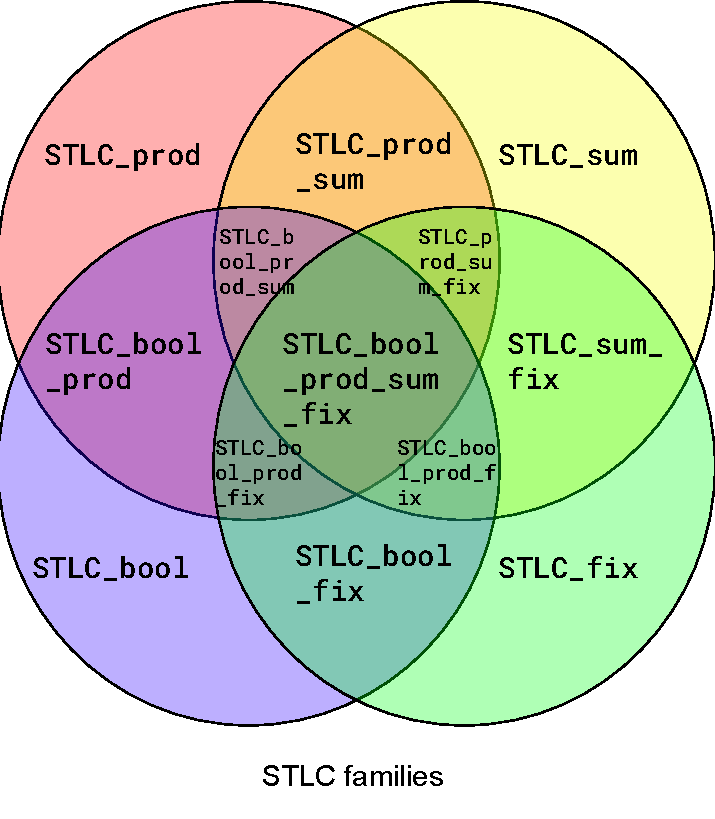
\includegraphics[width=0.5\textwidth]{coqexmaple/Mixin-Venn-Diagram.pdf}
\caption{Example STLC extended with product, and Mixin with \cref{fig:STLC-example2}}
\end{wrapfigure}

We start with the very basic type safety proof of STLC, largely adapted
from Software Foundation~\cite{pierce2014software}, which is also one of
the primal motivating example of this project. 


Our emphasis here is that, we singled out some language features from
STLC and prove the type safety for each feature separately, following
the style of the examples in MTC~\cite{delaware2013,forsta2020}.
And we use a \textit{not-yet-formally-defined} \textbf{mixin} feature
to mix the semantics and properties of language features---product
, boolean (in \cref{fig:STLC-example}), sum type and iso-recursive type---with vanilla STLC.



Using this example,
we hope one day we can say precisely, \textit{a programming language feature itself is a
piece of data/inheritance judgement/inherited family}. Compared with MTC,
our example uses small-step operational semantics\YZ{Does MTC not define a small-step operational semantics for STLC?}\EDJreply{I thought they use big step with fuel. Though Coq a la carte use small-step in one example} by exploiting
extensible inductive types. 

Most of the proof and computation are directly adapted
from the one in Software Foundation, resulting in a similarly accessible proof, while the proof for each extended feature are scattered in the extended families resulting better modularity. One kind of examples is about the computation, for example, substitution functions. Substitutions dealing with product and projection are defined in the corresponding children family. This is mainly done by inheriting and extending the handler family from the parents. The other kind of examples are about propositions and we directly use "(Extend) FTheorem" to handle them. In these cases we don't need to additionally define a auxillary handler family like we did for substitution---we simply use "Extend FTheorem" and our plugin will prepare the goals to prove. At the end, it will look like scattered proof scripts in a modular manner.
For example, the proof on progress on product projection is carried out in the children family that extend "tm" with products. \YZ{Can you say more about how your plugin enables more code reuse and modularity?}\EDJreply{please check}
% In related work, Coq/Metatheory a la carte/Tion embedding can be emphasized as a more "semantic approach" because they encode the meaning using a special design pattern (for example, open recursive inductive type for extension), compared to our more syntactic approach. Their advantage is the transferability of this technique accross different proof assistants, and their disadvantage is that their approach are less accessible and unfriendly to amateur Coq users---which can be reflected from the distance of their approach and text-book Software Foundation proof. 

% We have problem on inversion lemma. Check if it is the same problem as MTC
We use "Closing Fact" to state and prove the inversion lemma instead of
using the extensible proving mechanism "FTheorem". The reasons are that
(1) it introduces much less boilerplate code because the proof for these
inversion lemmas should be just simple case analysis and we should rely
on Coq to generate most of the boilerplate code;\YZ{I was under the impression that the plugin could not auto-generate Closing Facts or their proofs, no?}\EDJreply{I have make the above Closing Fact section more about this detail. Please check.} (2) it shouldn't bother us in the future
because any extension on the syntax should still satisfy these inversion
lemmas; (3) most importantly, we believe this inversion ``lemma'' should
be part of the definition of the syntax instead of considering the
syntax as a mere concrete inductive type. We should postulate this
inversion ``lemma'' like \textit{a constraint} and post-hoc-ly verify
that our inductive definition does satisfy the constraint, which is
exactly what we expect from "Closing Fact". If directly working on inductive definition doesn't bring us benefit during proof engineering, then decompose the property (the constraint) with the concrete definition might be a good idea.

Our formulation for bare STLC is around 400+ LOCs; each families implementing product and boolean features both take around 300+ LOCs. 
% need comparison with the original implementation

The biggest difference in the proof script comes from the fact that we
are handling ``extensible'' inductive types instead of real inductive
types, and thus the inversion tactic is not working and we have to manually
create inversion lemmas. 

Another difference comes from the fact that we need to use "Closing
Fact" to manually verify the computational rules for each recursor and
use tactics to ``run'' the recursor by repeatedly "rewrite" using those
verified computational rules. This part is possible to be automatically
generated by the plugin, but still it will require propositional 
computational rules.  What's more, we don't yet support the \mintinline{Coq}{Hint}. These three differences on experience lead to a mild code bloat. 

\subsection{Abstract Interpreters for \texttt{Imp}}\YZ{Try to have two runnable interpreter -- choose another simple one like constant propagation. and remove LangMore}
The second example is adapted and modified from \citet{zm2017}.
Contrary to our first example, here, we use a big-step interpreter with fuel
as the operational semantics of an imperative language with
side effects, and we specify the abstract interpretation and prove its
soundness, with some postulation on both computation and property. Then we instantiate our abstract interpretation with two concrete computation---one for type inference and the other for constant propagation. Our analyzer will return the analysis result about the end of the program, e.g. our constant propagator will return what constant value each variable is at the end of the program. Thanks to the compilation to Coq module, we can directly run the resulting
abstract interpreters.

% Then we extend the base language with new features, and we instantiate
% the postulation on computation for
% abstract interpreters.


\begin{figure}[!htb]
  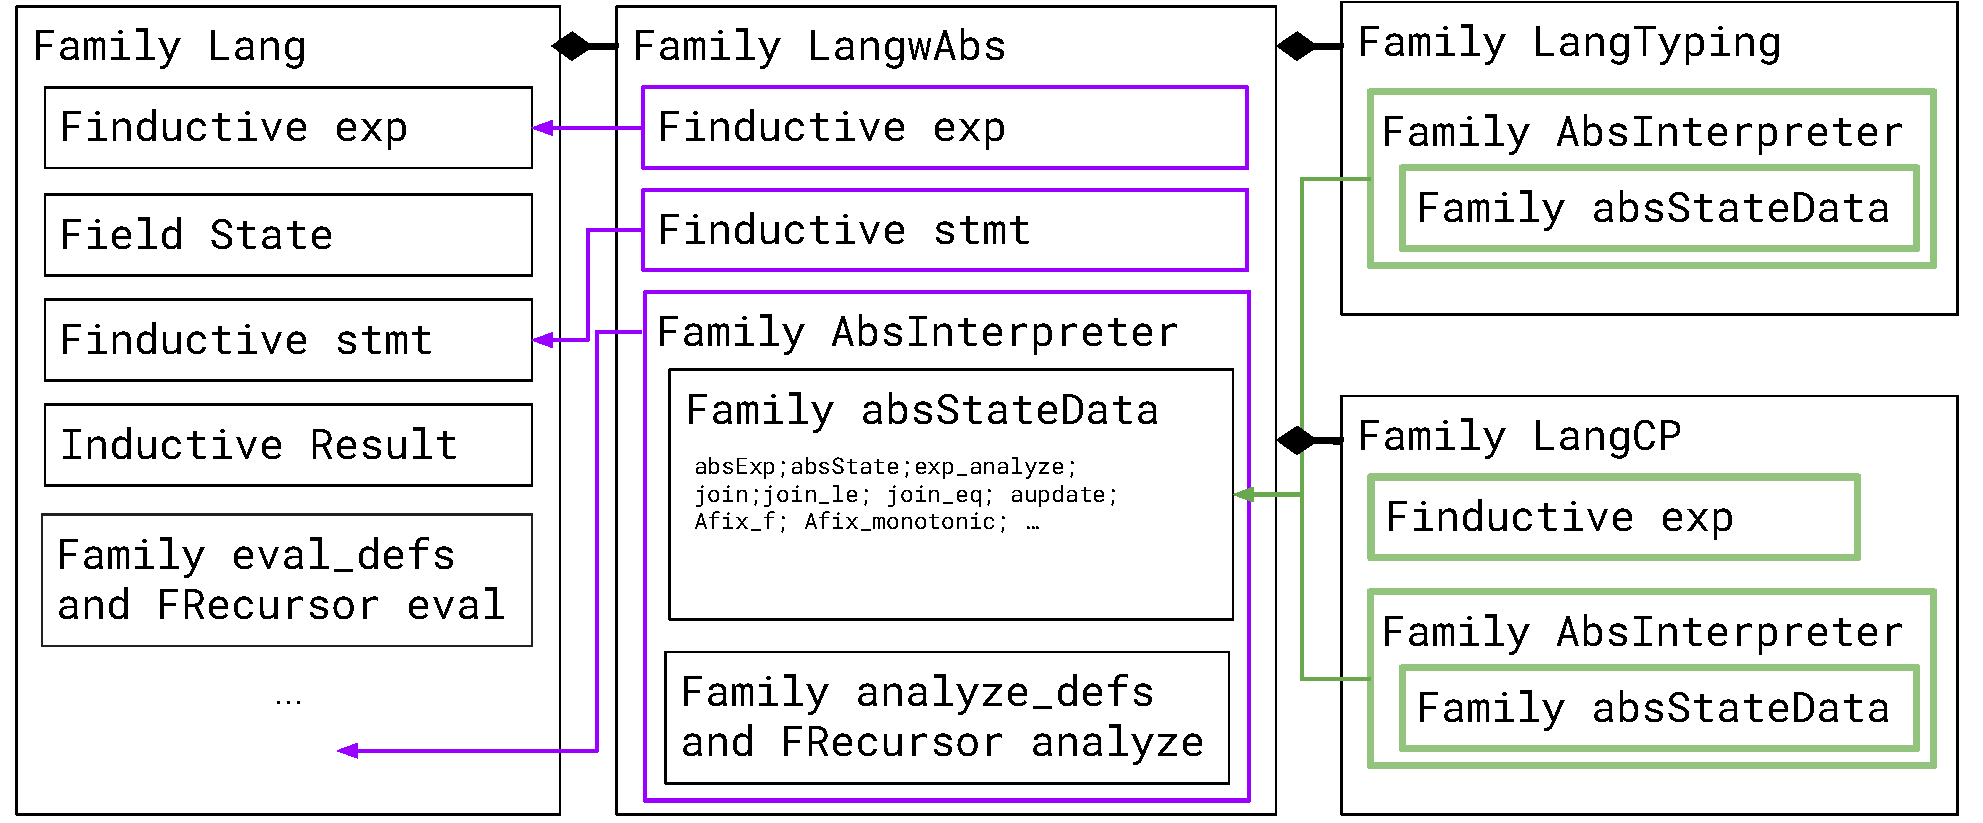
\includegraphics[width=\columnwidth]{coqexmaple/Family-Lang-Imp3.pdf}
  \caption{Inheritance Diagram for Abstract Interpretation Example. Black arrows are inheritance. Purple arrow are extending. Green arrows mean there are overriding.}\label{fig:abstract-interpretation-example}
\end{figure}

We construct four families, illustrated in \cref{fig:abstract-interpretation-example}.\YZ{Why is it useful to define these concrete and abstract interpreters as an inheritance chain?}\EDJreply{I don't think these examples are here to show the example themselves are useful. They are here to show family inheritance is useful, and can extend stuff to all sorts of things. I also add some details below on how each family can be extended and what each family means.}\YZreply{Why is it desired to define the abstract interpreter as an extension of the concrete interpreter family? What is lost by putting the two interpreters in the same family?}\EDJreply{Nothing is lost. This is just simulating people starting with bare (big-step) operational semantic. Because they may not working on abstract interpretation from the first place. Those people may extend "Lang" with other stuff like another type-safety proof or something.}
The first family "Lang" define the big step operator (using fuel) of a
while language, with expression and stmt defined upon expression. Final "Result" can be error, "out-of-fuel" or a legitmate "State". It takes about 200 LOCs. 
% We
% can
\YZ{In general, in a result section like this, you want to show what
you *have done* rather than what you *can do*.}\EDJreply{Ok. deleted. I initially want to emphasize ``I **can** use arbitrary implementation for this environment mapping interface'' but I don't know how to say that without using ``can''.}
% swap the implementation of "State" to have different memory/state
% management by extending family "Lang".
\YZ{What is 'different
memory/state management'?}\EDJreply{Actually I should say environment mapping/dictionary. I instantiate it with function(closure) as environment mapping in "LangRun". It is possible to use other mapping like Coq's primitive dictionary.}

The second family "LangwAbs" define the abstract interpreter for "Lang" in "LangwAbs.AbsInterpreter",
together with a bunch of postulates as a big sealed family "absStateData". Then we prove the correctness of the
abstract interpretation function "analyze". It takes about 300+ LOCs. This example shows how
to use family inheritance to extend a concrete interpreter with abstract
interpreters. 
% This example also shows in this family polymoprhism framework we can reason about "Lang" with computation details being abstracted. 

% The third Family "LangMore" extend "LangwAbs" with nat constant and
% addition, and if-then-else control flow, of course retaining all the
% soundness theorem. It takes about 200+ LOCs. This is one example of
% using family inheritance to support new language feature, and compatible
% with the existent reasoning in "LangwAbs.AbsInterpreter". 

The third family and the fourth family "LangTyping" and "LangCP" instantiate some of the postulates of the
"LangwAbs" and recover computational information of "analyze". The corresponding fields in "absStateData" is overridden by a concrete definition. The resulting abstract interpreter is expected
to act as a type-analyzer and constant-propagator respectively. It takes about 200+ LOCs. 
% These are two examples of instantiate the detail computation of abstract interpretation. 


And at the end, the compiled module for "LangTyping" and "LangCP" is put into tests over simple queries. These "LangTyping" and "LangCP" also illustrates that we still have
computability in the presence of family.\YZ{Mention the alternative approach of using parameterized modules.}\EDJreply{What. I don't have that version. My earlier version without family is not extensible, just a POC to see if the proof idea itself is correct.}

\subsection{An Extensible Decision Procedure for Parsing}
The third example is a decision procedure for parsing, based on the fact that, we can use Cop's Inductive Facility to encode CFG rules. Thus extensible inductive family corresponds to extensible CFG rules. For example, indexed type \mintinline{Coq}{is_prog : strs → Type} is a predicate asserting if a token list is a syntactically well-formed program.

\begin{figure}[!htb]
  \lstset{
      basicstyle=\fontsize{8}{8.5}\ttfamily,
  % numbers=left,
  }
  
  \begin{minipage}{\textwidth}
  \begin{multicols}{2}
  

  \definecolor{codecomment-color}{HTML}{0DA3FF}
  
  \begin{lstlisting}
  FInductive is_prog : strs -> Type := 
  | ip_seq : forall a b, is_prog a -> is_prog b 
      -> is_prog (a ++ [";"] ++ b) 
  | ip_assign : forall i e, is_atom i -> is_exp e 
      -> is_prog ([i; "="] ++ e).  
  \end{lstlisting}
  
  % \makeline[0pt]{Parser-exmp-before-start}{Parser-exmp-before-end}[codecomment-color!50]
  
  \columnbreak
  \definecolor{codecomment-color}{HTML}{5D030F}
  
  \begin{lstlisting}
  FInductive is_prog : strs -> Type += 
  | ip_if : forall a b, is_exp a -> is_prog b 
      -> is_prog (["if"] ++ a ++ ["then"] ++ b). 
  \end{lstlisting}
  
  
  
  % \makeline[.5\textwidth+9pt]{Parser-exmp-after-start}{Parser-exmp-after-end}[codecomment-color!50]
  
  \end{multicols}
  \end{minipage}
  \caption{"is_prog" and its extension}
  \end{figure}



We prove decidability of "is_prog" via strong induction on the length. The non-trivial part is  the inductive step, i.e. we need to show "is_prog" is ``conditionally decidable'':
\begin{minted}[fontsize=\footnotesize]{Coq}
  (forall e, len e < len s -> (is_prog e) + (is_prog e -> False)) -> (is_prog s) + (is_prog s -> False)
\end{minted}

This proposition should hold due to the shape of the inductive definition---because we can translate the definition of "is_prog" into an equivalence to a big disjunction: 
\begin{minted}[fontsize=\footnotesize]{Coq}
(∃ a ∃ b , is_prog a /\ is_prog b /\ s = a ++ [";"] ++ b)
\/ (∃ i ∃ e, is_atom i /\ is_exp e /\ s = i ++ [":="] ++ e) 
... 
<-> is_prog s
\end{minted}
Then decidability is immediate via this equivalence, since on LHS every sub token list has length strictly smaller than "s". 

However, when maintaining this equivalence proof through out different families---calling this big disjunction on LHS as \mintinline{Coq}{alg_is_prog : strs -> Type}---"alg_is_prog" is changing when "is_prog" extends. Thus "alg_is_prog" should be encoded as an overridable field. 

We will have challenges maintaining this equivalence proof. From left to right (soundness), we can have incremental construction and proof reuse throughout different families---we can easily prove "is_prog l" using each constructor. However, from right to left (completeness), the proof from the parent family cannot be reused in the children as "alg_is_prog" is changing and the proposition itself is changing. So we use "overridable" to organize the proof of completeness. 

It is around 750 lines of codes using Family facility and around 900 lines of code using vanilla Coq. Around 350 lines of them are public helper function used by both implementations.

% Then we provide an overridable predicate \mintinline{Coq}{alg_is_prog : strs -> Type},\YZ{Why does it need to be overridden?}\EDJreply{Basically alg_is_prog is a big disjunction list, corresponding to each of the constructor of }
% decidable provided the inductive hypothesis and sound \& complete w.r.t. to the specification \mintinline{Coq}{alg_is_prog e  <-> is_prog e}.  "alg_is_prog e" will be a big disjunction, of which each disjunct $P_i$ corresponds to the argument of one constructor of "is_prog" (each CFG rule). Thus once "is_prog" is extended, we need to disjunct "alg_is_prog" with more condition, thus overridable.  We require extension to take care of the disjuncts, their soundness \& completeness and the conditional decidablity.

% Among them, completeness \mintinline{Coq}{is_prog e -> alg_is_prog e} is
% the most challenging part. This is proved by recursion on the predicate
% "is_prog e", but none of the handler on "is_prog" will be reused
% because \mintinline{Coq}{alg_is_prog e} is overriden during
% inheritance.


% Unlike completeness, other parts of the construction, including
% soundness and and conditional decidability can be reused easily.
\YZ{But is the reusability achieved through a derived family's reusing handlers in the base family? Doesn't sound like it because the induction seems to be on strs.}\EDJreply{to prove something like alg_is_prog e -> is_prog e is not doing induction on string. It is just unfolding definition. \\ 
alg_is_prog is a big disjunction, alg_is_prog e = p1 e \/ p2 e\/ ..., and during overriding this disunction list is increasing. \\
So we organize the program by proving ``p1 e -> is_prog e'', ``p2 e -> is_prog e''. Everytime this disjunction list is increasing during overriding, the old proof ``p1 e -> is_prog e'' is reused in the new .}



\section{Conclusion}
\label{sec:conclusion}

\setlength{\bibsep}{.8ex}
\bibliographystyle{tex-macros/ACM-Reference-Format.bst}
\bibliography{refs.bib}

\appendix

\section{Metatheory in (pseudo-)Agda}
We make three agda source code files (publicly and anonymously) openly avaliable, and they include the corresponding QIIT syntax definition and models. 

For syntax, please check \href{https://drive.google.com/file/d/1aoG67rmXzP_x1MvZCIN3do0sucyqjwkn/view?usp=sharing}{here}.

For consistency model, please check \href{https://drive.google.com/file/d/1pNhnn125P5byAHDaSIlpbxMvr1F-9FRo/view?usp=sharing}{here}.

For canonicity model, please check \href{https://drive.google.com/file/d/1R6C7QNfyu8fbl6LE2ruvpqZ_ZDSRVo0c/view?usp=sharing}{here}.

We suggest using editors with proper syntax highlighting, e.g. VSCode with agda-code plugins.